\documentclass[preprint,aps,pra,onecolumn]{revtex4-1} %reprint
%\tightenlines

%\draft
\usepackage{etex}
\usepackage{amsmath}
\usepackage{bm}
\usepackage{bbm}
\usepackage{listings}
% % \textwidth 16cm \textheight 23.5cm
% \renewcommand{\baselinestretch}{1.2}
\usepackage{graphicx}
\usepackage{graphics}
\usepackage{epsfig}
\usepackage{color}
\usepackage{multirow}
\usepackage[colorlinks]{hyperref}
\usepackage{fancyhdr}
\usepackage{calc}
\usepackage{natbib} %[numbers]
\usepackage{bibentry}
% underline tool
\usepackage[normalem]{ulem}
\usepackage[usenames,dvipsnames]{xcolor}
%\uline{foo}	Underlines foo
%\uuline{foo}	Double underlines foo
%\uwave{foo}	Underlines foo with a wavy line
%\sout{foo}	Strikesout foo
%\xout{foo}	Crosses out foo with ¡®/6¤7¡¯
% triple lines in colors
\makeatletter
\newcommand\uuuline{\bgroup\markoverwith%
   {%
     \textcolor{red}{\rule[-0.5ex]{2pt}{0.4pt}}%
     \llap{\textcolor{blue}{\rule[-0.7ex]{2pt}{0.4pt}}}%
     \llap{\textcolor{green}{\rule[-0.9ex]{2pt}{0.4pt}}}%
   }%
   \ULon}
\makeatother


\usepackage{amsmath,soul} % underline with a number
% usage example: $\underset{4}{\text{\ul{This is short text}}}$
% another package to use, but did not work for me.
% From: http://tex.stackexchange.com/questions/45341/labeling-underlined-text-over-multiple-lines
%\usepackage{soulpos}
%\ulposdef{\ulnumaux}{%
%   $\underset{\saveulnum}{\rule[-.7ex]{\ulwidth}{.4pt}}$}
%
%\newcommand{\ulnum}[2]{%
%  \def\saveulnum{#1}%
%  \ulnumaux{#2}}

% todo list and commands
\usepackage{todonotes}
%% to avoid the conflict with amths package % not working
%\makeatletter
%\providecommand\@dotsep{5}
%\makeatother
%\listoftodos\relax
\usepackage{makeidx}
\allowdisplaybreaks
% for eps transfering to pdf.
\usepackage[update,prepend]{epstopdf}
\usepackage{ifpdf}

\ifpdf
   \usepackage{graphicx}
   \usepackage{epstopdf}
   \epstopdfsetup{suffix=}
   \DeclareGraphicsRule{.eps}{pdf}{.pdf}{`epstopdf #1}
   \pdfcompresslevel=9
\else
   \usepackage{graphicx}
\fi
% subfig
%\usepackage{mwe}
\usepackage{subfig}
% to fix a figure's position using [H] option of thec figure.
\usepackage{float}
% to use \lesssim and other math symbols
\usepackage{amssymb}


% self-defined short-cuts and commands

% packages we need for judging the operating system
% compile your tex file with option -shell-escape is required: 
% e.g. xelatex -shell-escape file.tex
\usepackage{pdftexcmds}
\usepackage{catchfile}
\usepackage{ifluatex}
\usepackage{ifplatform}

% self-definition for short hand

% symbols and math operators
\DeclareMathOperator{\spn}{span}
\DeclareMathOperator{\tr}{tr}
% definition of grammars % formats related
\definecolor{MyDarkGreen}{rgb}{0.0,0.4,0.0}
\newcommand{\greek}[1]{{\selectlanguage{greek}#1}} % will look for grmn font: tlmgr install cbfonts (65 MB)

% functions
\newcommand{\sn}{\mathrm{sn}}
\newcommand{\cn}{\mathrm{cn}}
\newcommand{\dn}{\mathrm{dn}}

% constants
\newcommand{\invtpi}{\frac{1}{2\pi}}

% vectors and tensors
\def\en{\mathbf{e}_n}
\def\eye{\mathbf{I}}
\newcommand\lvec[1]{\accentset{\leftarrow}{#1}}
% math font
\newcommand{\bmc}[1]{\boldsymbol{\mathcal{#1}}}

% derivatives and integrals
% ordinary derivatives
\newcommand{\drv}{\mathrm{d}}
\newcommand{\dt}[1]{\frac{{\mathrm d} {#1}}{{\mathrm d}t}}
\newcommand{\dx}[1]{\frac{{\mathrm d} {#1}}{{\mathrm d}x}}
\newcommand{\dtau}{\frac{{\mathrm d} }{{\mathrm d}\tau}}
\newcommand{\dd}[2]{\frac{{\mathrm d} {#1}}{{\mathrm d} {#2}}}
\newcommand{\sdt}[1]{\frac{{\mathrm d}^2 {#1}}{{\mathrm d}t^2}}
\newcommand{\sdx}[1]{\frac{{\mathrm d}^2 {#1}}{{\mathrm d}x^2}}
\newcommand{\sdd}[2]{\frac{{\mathrm d}^2 {#1}}{{\mathrm d}{#2}^2}}
\newcommand{\ddn}[3]{\frac{{\mathrm d}^{#1} #2}{{\mathrm d} #3 ^{#1}}}

% partial derivatives
\newcommand{\pt}[1]{\frac{\partial {#1}}{\partial t}}
\newcommand{\px}[1]{\frac{\partial {#1}}{\partial x}}
\newcommand{\pp}[2]{\frac{\partial {#1}}{\partial {#2}}}
\newcommand{\spt}[1]{\frac{\partial^2 {#1}}{\partial t^2}}
\newcommand{\spx}[1]{\frac{\partial^2 {#1}}{\partial x^2}}
\newcommand{\spp}[2]{\frac{\partial^2 {#1}}{\partial {#2}^2}}
\newcommand{\ppn}[3]{\frac{\partial^{#1} #2}{\partial #3 ^{#1}}}
% integrals
\newcommand{\intl}[2]{\int_0^\infty\! #1 \mathrm{d}#2}
\newcommand{\intf}[2]{\int_{-\infty}^\infty\! #1 \mathrm{d}#2}


% quantum operators
\newcommand{\ssp}{\braket{\sigma^{+}(t)\sigma^{-}(t)}}
\newcommand{\aap}{\braket{a^{\dagger}(t)a(t)}}
\newcommand{\as}{\braket{a^{\dagger}(t)\sigma^{-}(t)}}
\newcommand{\sa}{\braket{a(t)\sigma^{+}(t)}}
\newcommand{\Hssp}{\braket{\sigma^{+}\sigma^{-}}}
\newcommand{\Haap}{\braket{a^{\dagger}a}}
\newcommand{\Has}{\braket{a^{\dagger}\sigma^{-}}}
\newcommand{\Hsa}{\braket{a\sigma^{+}}}
\newcommand{\adag}{a^{\dagger}}
\newcommand{\sigm}{\sigma^{-}}
\newcommand{\sigp}{\sigma^{+}}
\newcommand{\sigz}{\sigma^{z}}
\newcommand{\gp}{\gamma^{\prime}}
\newcommand{\oal}{\omega_a-\omega_0}
\newcommand{\ocl}{\omega_c-\omega_0}


% Green function related
\def\GFT{\overline{\bf G}}
\def\IT{\overline{\bf I}}
\def\TT{\overline{\bf T}}
\def\MT{\overline{\bf M}}
\def\AT{\overline{\bf A}}
\def\BT{\overline{\bf B}}
\def\fT{\overline{\bf f}}
\def\LT{\overline{\bf L}}
\def\alphaT{\overline{\bf \alpha}}
\def\GFTr{\overline{\bf G}\left(\mathbf{r},\mathbf{r}'\right)}
\def\GFTrw{\overline{\bf G}\left(\mathbf{r},\mathbf{r}';\omega\right)}
\def\rarg{\left(\mathbf{r}\right)}
\def\rargw{\left(\mathbf{r};\omega\right)}
\def\rrarg{\left(\mathbf{r},\mathbf{r}'\right)}
\def\rrargw{\left(\mathbf{r},\mathbf{r}';\omega\right)}
\def\rk{\left(\mathbf{r}_k\right)}
\def\rn{\left(\mathbf{r}_n\right)}
\def\rnrn{\left(\mathbf{r}_n,\mathbf{r}_n\right)}
\def\rnrk{\left(\mathbf{r}_n,\mathbf{r}_k\right)}
\def\rkrk{\left(\mathbf{r}_k,\mathbf{r}_k\right)}
\def\rkrn{\left(\mathbf{r}_k,\mathbf{r}_n\right)}
\def\br{\mathbf{r}}
\def\Erw{\hat{\mathbf{E}}(\mathbf{r},\omega)}
\def\E0{\hat{\mathbf{E}}^{(0)}(\mathbf{r},\omega)}
\def\Arw{\hat{\mathbf{A}}(\mathbf{r},\omega)}
\def\Snw{\hat{\mathbf{S}}_n(\omega)}
\def\Unw{\mathbf{U}_n(\omega)}
\def\unw{U_n(\omega)}
\def\Alphanw{{\bm \alpha}_n(\omega)}
\def\Krrw{\mathbf{K}(\mathbf{r},\mathbf{r}',\omega)}
\def\Krrnw{\mathbf{K}(\mathbf{r},\mathbf{r}_n,\omega)}
\def\GTrrw{\mathbf{G}^T(\mathbf{r},\mathbf{r}',\omega)}
\def\Grrw{\mathbf{G}(\mathbf{r},\mathbf{r}',\omega)}
\def\Gn{\mathbf{G}^n}
\def\Gm1{\mathbf{G}^{n-1}}
\def\GN{\mathbf{G}^N}
\def\G0{\mathbf{G}^0}
\def\G1{\mathbf{G}^1}
\def\Gi{\mathbf{G}^i}
\def\flamr{\mathbf{f}_\lambda(\mathbf{r})}
\def\rrn{\mathbf{r},\mathbf{r}_n}
\def\rnrn{\mathbf{r}_n,\mathbf{r}_n}
\def\rr{\mathbf{r},\mathbf{r}'}


% braket.sty          Macros for Dirac bra-ket <|> notation and sets {|}
%
\def\bra#1{\langle{#1}\rvert}%{\mathinner{\langle{#1}\rvert}}
\def\ket#1{\lvert{#1}\rangle}%{\mathinner{\lvert{#1}\rangle}}
\def\braket#1{\mathinner{\langle{#1}\rangle}}
\def\Bra#1{\left<#1\right|}
\def\Ket#1{\left|#1\right>}
{\catcode`\|=\active
  \gdef\Braket#1{\left<\mathcode`\|"8000\let|\BraVert {#1}\right>}}
\def\BraVert{\egroup\,\mid@vertical\,\bgroup}
{\catcode`\|=\active
  \gdef\set#1{\mathinner{\lbrace\,{\mathcode`\|"8000\let|\midvert #1}\,\rbrace}}
  \gdef\Set#1{\left\{\:{\mathcode`\|"8000\let|\SetVert #1}\:\right\}}}
\def\midvert{\egroup\mid\bgroup}
\def\SetVert{\egroup\;\mid@vertical\;\bgroup}
% Some stuff deleted
% Macros for Dirac bra-ket <|> notation
%\def\bra#1{\mathinner{\langle{#1}|}}
%\def\ket#1{\mathinner{|{#1}\rangle}}
\def\Braket#1#2{\mathinner{\langle{#1}\! \mid\! {#2} \rangle}}
\def\ketbra#1{\ket{#1}\!\!\bra{#1}}
\newcommand{\Ketbra}[2]{\ket{#1}\!\!\bra{#2}}
\def\sandwich#1#2{\bra{#1}\! #2 \! \ket{#1}}
\def\Sandwich#1#2#3{\bra{#1}\! #2\! \ket{#3}}
%
% END  braket.sty     Macros for Dirac bra-ket <|> notation and sets {|}


%% Ben's shortcuts.
% Equation, citation, and labeling macros
%========================================================================================
\newcommand{\erf}[1]{Eq.~(\ref{#1})}
\newcommand{\frf}[1]{Fig.~\ref{#1}}
\newcommand{\srf}[1]{Sec.~\ref{#1}}
\newcommand{\nn}{\nonumber}
\newcommand{\mbf}[1]{\mathbf{#1}}
%========================================================================================
% General quantum mechanics macros
%========================================================================================
\newcommand{\ip}[2]{\langle{#1}|{#2}\rangle}
\newcommand{\op}[2]{\ket{#1}\bra{#2}}
\newcommand{\enavg}[1]{\mathrm{E}\sq{#1}}
\newcommand{\gravg}[1]{\mathbb{E}\sq{#1}}
\newcommand{\expt}[1]{\langle{#1}\rangle}
\newcommand{\dg}{^\dagger}
\newcommand{\smallfrac}[2]{\mbox{$\frac{#1}{#2}$}}
\newcommand{\emn}[1]{ \mathbbm{E}_{#1} }
\newcommand{\Tr}{\mbox{Tr}}
%\newcommand{\tensor}[1]{\boldsymbol{#1}}%{\overset{\leftrightarrow}{#1}}
%========================================================================================
% Famous physicists
%========================================================================================
\newcommand{\sch}{Schr\"odinger}
\newcommand{\hei}{Heisenberg }
\newcommand{\ein}{Einstein }
\newcommand{\str}{Stratonovich }
%========================================================================================
% Dirac notation and commutators
%========================================================================================
\newcommand{\norm}[1]{\lvert #1 \rvert}
\newcommand{\opnorm}[1]{\lVert #1 \rVert}
%\newcommand{\ket}[1]{\lvert #1 \rangle}
%\newcommand{\bra}[1]{\langle #1 \rvert}
\newcommand{\bravket}[2]{\langle\, #1\,\vert\, #2 \,\rangle}
\newcommand{\av}[1]{\left\langle #1 \right\rangle}
\newcommand{\proj}[1]{\ket{#1}\!\bra{#1}}
\newcommand{\commut}[2]{[\ssp #1,\,#2\ssp]}
\newcommand{\anticommut}[2]{\{\ssp #1,\,#2\ssp\}}
% big Dirac notation and commutators
\newcommand{\bnorm}[1]{\big\lvert #1 \big\rvert}
\newcommand{\bopnorm}[1]{\big\lVert #1 \big\rVert}
\newcommand{\bket}[1]{\big\lvert\, #1\, \big\rangle}
\newcommand{\bbra}[1]{\big\langle\, #1\, \big\rvert}
\newcommand{\bbraket}[2]{\big\langle\, #1\,\big\vert\, #2 \,\big\rangle}
\newcommand{\bav}[1]{\bigl\langle #1 \bigr\rangle}
\newcommand{\bproj}[1]{\bket{#1}\!\bbra{#1}}
\newcommand{\bcommut}[2]{\big[\ssp #1,\,#2\ssp\big]}
\newcommand{\banticommut}[2]{\big\{\ssp #1,\,#2\ssp\big\}}
% Big Dirac notation and commutators
\newcommand{\Bnorm}[1]{\Big\lvert #1 \Big\rvert}
\newcommand{\Bopnorm}[1]{\Big\lVert #1 \Big\rVert}
\newcommand{\Bket}[1]{\Big\lvert\, #1\, \Big\rangle}
\newcommand{\Bbra}[1]{\Big\langle\, #1\, \Big\rvert}
\newcommand{\Bbraket}[2]{\Big\langle\, #1\,\Big\vert\, #2 \,\Big\rangle}
\newcommand{\Bav}[1]{\Bigl\langle #1 \Bigr\rangle}
\newcommand{\Bproj}[1]{\Bket{#1}\!\Bbra{#1}}
\newcommand{\Bcommut}[2]{\Big[\ssp #1,\,#2\ssp\Big]}
\newcommand{\Banticommut}[2]{\Big\{\ssp #1,\,#2\ssp\Big\}}
%========================================================================================
% Nanofiber interface macros
%========================================================================================
\newcommand{\expect}[1]{\big\langle #1 \big\rangle}
\newcommand{\expects}[1]{\langle #1 \rangle}
\newcommand{\melement}[3]{\langle #1 \lvert #2 \rvert #3 \rangle}
\newcommand{\Ip}[2]{\left\langle {#1},{#2} \right\rangle}
\newcommand{\modsq}[1]{\lvert #1 \rvert^2}
\newcommand{\normsq}[1]{\lVert #1 \rVert^2}
\newcommand{\grad}{\nabla}
\newcommand{\partialD}[2]{\frac{\partial #1}{\partial #2}}

\newcommand{\peakprobe}{\mathcal{E}_0}
\newcommand{\eff}{\text{eff}}
\newcommand{\varFz}{\big( \Delta F_z^{0} \big)^2}
\newcommand{\varFzText}{( \Delta F_z^{0} )^2}
\newcommand{\varFzLG}{( \Delta F_z^{00} )^2}

\newcommand{\rperp}{\mathbf{r}_\perp}
\newcommand{\talphan}{\overset{\leftrightarrow}{\alpha}{}^{(n)}}
\newcommand{\talphanOp}{\hat{\overset{\leftrightarrow}{\alpha}}{}^{(n)}}

%\newcommand{\Cstrength}{ \chi^{(1)}\sqrt{ \dot{N}_L } }
%\newcommand{\CstrengthSq}{ \big(\chi^{(1)} \big)^2 \dot{N}_L }
\newcommand{\Cstrength}{ \sqrt{\kappa} }
\newcommand{\CstrengthSq}{ \kappa }
%========================================================================================
%  Spacing macros
%========================================================================================
%\newcommand{\ssp}{\hspace{0.4pt}}%small horizontal space
\newcommand{\nsp}{\hspace{-0.7pt}}%negative horizontal space
%========================================================================================




% For faster processing, load Matlab syntax for listings
\lstloadlanguages{Matlab}% use listings package
\lstset{language=Matlab,
        frame=single,
        basicstyle=\small\ttfamily,
        keywordstyle=[1]\color{Blue}\bf,
        keywordstyle=[2]\color{Purple},
        keywordstyle=[3]\color{Blue}\underbar,
        identifierstyle=,
        commentstyle=\usefont{T1}{pcr}{m}{sl}\color{MyDarkGreen}\small,
        stringstyle=\color{Purple},
        showstringspaces=false,
        tabsize=5,
        % Put standard MATLAB functions not included in the default
        % language here
        morekeywords={xlim,ylim,var,alpha,factorial,poissrnd,normpdf,normcdf},
        % Put MATLAB function parameters here
        morekeywords=[2]{on, off, interp},
        % Put user defined functions here
        morekeywords=[3]{FindESS},
        morecomment=[l][\color{Blue}]{...},
        numbers=left,
        firstnumber=1,
        numberstyle=\tiny\color{Blue},
        stepnumber=5
        }
        
        
        
% Includes a figure
% The first parameter is the label, which is also the name of the figure
%   with or without the extension (e.g., .eps, .fig, .png, .gif, etc.)
%   IF NO EXTENSION IS GIVEN, LaTeX will look for the most appropriate one.
%   This means that if a DVI (or PS) is being produced, it will look for
%   an eps. If a PDF is being produced, it will look for nearly anything
%   else (gif, jpg, png, et cetera). Because of this, when I generate figures
%   I typically generate an eps and a png to allow me the most flexibility
%   when rendering my document.
% The second parameter is the width of the figure normalized to column width
%   (e.g. 0.5 for half a column, 0.75 for 75% of the column)
% The third parameter is the caption.
\newcommand{\scalefig}[3]{
  \begin{figure}[ht!]
    % Requires \usepackage{graphicx}
    \centering
    \includegraphics[width=#2\columnwidth]{#1}
    %%% I think \captionwidth (see above) can go away as long as
    %%% \centering is above
    %\captionwidth{#2\columnwidth}%
    \caption{#3}
    \label{#1}
  \end{figure}}
% judge platform and include correct definiation package
%\ifwindows
%	%% self-definition for short hand

% symbols and math operators
\DeclareMathOperator{\spn}{span}
\DeclareMathOperator{\tr}{tr}
% definition of grammars % formats related
\definecolor{MyDarkGreen}{rgb}{0.0,0.4,0.0}
\newcommand{\greek}[1]{{\selectlanguage{greek}#1}} % will look for grmn font: tlmgr install cbfonts (65 MB)

% functions
\newcommand{\sn}{\mathrm{sn}}
\newcommand{\cn}{\mathrm{cn}}
\newcommand{\dn}{\mathrm{dn}}

% constants
\newcommand{\invtpi}{\frac{1}{2\pi}}

% vectors and tensors
\def\en{\mathbf{e}_n}
\def\eye{\mathbf{I}}
\newcommand\lvec[1]{\accentset{\leftarrow}{#1}}
% math font
\newcommand{\bmc}[1]{\boldsymbol{\mathcal{#1}}}

% derivatives and integrals
% ordinary derivatives
\newcommand{\drv}{\mathrm{d}}
\newcommand{\dt}[1]{\frac{{\mathrm d} {#1}}{{\mathrm d}t}}
\newcommand{\dx}[1]{\frac{{\mathrm d} {#1}}{{\mathrm d}x}}
\newcommand{\dtau}{\frac{{\mathrm d} }{{\mathrm d}\tau}}
\newcommand{\dd}[2]{\frac{{\mathrm d} {#1}}{{\mathrm d} {#2}}}
\newcommand{\sdt}[1]{\frac{{\mathrm d}^2 {#1}}{{\mathrm d}t^2}}
\newcommand{\sdx}[1]{\frac{{\mathrm d}^2 {#1}}{{\mathrm d}x^2}}
\newcommand{\sdd}[2]{\frac{{\mathrm d}^2 {#1}}{{\mathrm d}{#2}^2}}
\newcommand{\ddn}[3]{\frac{{\mathrm d}^{#1} #2}{{\mathrm d} #3 ^{#1}}}

% partial derivatives
\newcommand{\pt}[1]{\frac{\partial {#1}}{\partial t}}
\newcommand{\px}[1]{\frac{\partial {#1}}{\partial x}}
\newcommand{\pp}[2]{\frac{\partial {#1}}{\partial {#2}}}
\newcommand{\spt}[1]{\frac{\partial^2 {#1}}{\partial t^2}}
\newcommand{\spx}[1]{\frac{\partial^2 {#1}}{\partial x^2}}
\newcommand{\spp}[2]{\frac{\partial^2 {#1}}{\partial {#2}^2}}
\newcommand{\ppn}[3]{\frac{\partial^{#1} #2}{\partial #3 ^{#1}}}
% integrals
\newcommand{\intl}[2]{\int_0^\infty\! #1 \mathrm{d}#2}
\newcommand{\intf}[2]{\int_{-\infty}^\infty\! #1 \mathrm{d}#2}


% quantum operators
\newcommand{\ssp}{\braket{\sigma^{+}(t)\sigma^{-}(t)}}
\newcommand{\aap}{\braket{a^{\dagger}(t)a(t)}}
\newcommand{\as}{\braket{a^{\dagger}(t)\sigma^{-}(t)}}
\newcommand{\sa}{\braket{a(t)\sigma^{+}(t)}}
\newcommand{\Hssp}{\braket{\sigma^{+}\sigma^{-}}}
\newcommand{\Haap}{\braket{a^{\dagger}a}}
\newcommand{\Has}{\braket{a^{\dagger}\sigma^{-}}}
\newcommand{\Hsa}{\braket{a\sigma^{+}}}
\newcommand{\adag}{a^{\dagger}}
\newcommand{\sigm}{\sigma^{-}}
\newcommand{\sigp}{\sigma^{+}}
\newcommand{\sigz}{\sigma^{z}}
\newcommand{\gp}{\gamma^{\prime}}
\newcommand{\oal}{\omega_a-\omega_0}
\newcommand{\ocl}{\omega_c-\omega_0}


% Green function related
\def\GFT{\overline{\bf G}}
\def\IT{\overline{\bf I}}
\def\TT{\overline{\bf T}}
\def\MT{\overline{\bf M}}
\def\AT{\overline{\bf A}}
\def\BT{\overline{\bf B}}
\def\fT{\overline{\bf f}}
\def\LT{\overline{\bf L}}
\def\alphaT{\overline{\bf \alpha}}
\def\GFTr{\overline{\bf G}\left(\mathbf{r},\mathbf{r}'\right)}
\def\GFTrw{\overline{\bf G}\left(\mathbf{r},\mathbf{r}';\omega\right)}
\def\rarg{\left(\mathbf{r}\right)}
\def\rargw{\left(\mathbf{r};\omega\right)}
\def\rrarg{\left(\mathbf{r},\mathbf{r}'\right)}
\def\rrargw{\left(\mathbf{r},\mathbf{r}';\omega\right)}
\def\rk{\left(\mathbf{r}_k\right)}
\def\rn{\left(\mathbf{r}_n\right)}
\def\rnrn{\left(\mathbf{r}_n,\mathbf{r}_n\right)}
\def\rnrk{\left(\mathbf{r}_n,\mathbf{r}_k\right)}
\def\rkrk{\left(\mathbf{r}_k,\mathbf{r}_k\right)}
\def\rkrn{\left(\mathbf{r}_k,\mathbf{r}_n\right)}
\def\br{\mathbf{r}}
\def\Erw{\hat{\mathbf{E}}(\mathbf{r},\omega)}
\def\E0{\hat{\mathbf{E}}^{(0)}(\mathbf{r},\omega)}
\def\Arw{\hat{\mathbf{A}}(\mathbf{r},\omega)}
\def\Snw{\hat{\mathbf{S}}_n(\omega)}
\def\Unw{\mathbf{U}_n(\omega)}
\def\unw{U_n(\omega)}
\def\Alphanw{{\bm \alpha}_n(\omega)}
\def\Krrw{\mathbf{K}(\mathbf{r},\mathbf{r}',\omega)}
\def\Krrnw{\mathbf{K}(\mathbf{r},\mathbf{r}_n,\omega)}
\def\GTrrw{\mathbf{G}^T(\mathbf{r},\mathbf{r}',\omega)}
\def\Grrw{\mathbf{G}(\mathbf{r},\mathbf{r}',\omega)}
\def\Gn{\mathbf{G}^n}
\def\Gm1{\mathbf{G}^{n-1}}
\def\GN{\mathbf{G}^N}
\def\G0{\mathbf{G}^0}
\def\G1{\mathbf{G}^1}
\def\Gi{\mathbf{G}^i}
\def\flamr{\mathbf{f}_\lambda(\mathbf{r})}
\def\rrn{\mathbf{r},\mathbf{r}_n}
\def\rnrn{\mathbf{r}_n,\mathbf{r}_n}
\def\rr{\mathbf{r},\mathbf{r}'}


% braket.sty          Macros for Dirac bra-ket <|> notation and sets {|}
%
\def\bra#1{\langle{#1}\rvert}%{\mathinner{\langle{#1}\rvert}}
\def\ket#1{\lvert{#1}\rangle}%{\mathinner{\lvert{#1}\rangle}}
\def\braket#1{\mathinner{\langle{#1}\rangle}}
\def\Bra#1{\left<#1\right|}
\def\Ket#1{\left|#1\right>}
{\catcode`\|=\active
  \gdef\Braket#1{\left<\mathcode`\|"8000\let|\BraVert {#1}\right>}}
\def\BraVert{\egroup\,\mid@vertical\,\bgroup}
{\catcode`\|=\active
  \gdef\set#1{\mathinner{\lbrace\,{\mathcode`\|"8000\let|\midvert #1}\,\rbrace}}
  \gdef\Set#1{\left\{\:{\mathcode`\|"8000\let|\SetVert #1}\:\right\}}}
\def\midvert{\egroup\mid\bgroup}
\def\SetVert{\egroup\;\mid@vertical\;\bgroup}
% Some stuff deleted
% Macros for Dirac bra-ket <|> notation
%\def\bra#1{\mathinner{\langle{#1}|}}
%\def\ket#1{\mathinner{|{#1}\rangle}}
\def\Braket#1#2{\mathinner{\langle{#1}\! \mid\! {#2} \rangle}}
\def\ketbra#1{\ket{#1}\!\!\bra{#1}}
\newcommand{\Ketbra}[2]{\ket{#1}\!\!\bra{#2}}
\def\sandwich#1#2{\bra{#1}\! #2 \! \ket{#1}}
\def\Sandwich#1#2#3{\bra{#1}\! #2\! \ket{#3}}
%
% END  braket.sty     Macros for Dirac bra-ket <|> notation and sets {|}


%% Ben's shortcuts.
% Equation, citation, and labeling macros
%========================================================================================
\newcommand{\erf}[1]{Eq.~(\ref{#1})}
\newcommand{\frf}[1]{Fig.~\ref{#1}}
\newcommand{\srf}[1]{Sec.~\ref{#1}}
\newcommand{\nn}{\nonumber}
\newcommand{\mbf}[1]{\mathbf{#1}}
%========================================================================================
% General quantum mechanics macros
%========================================================================================
\newcommand{\ip}[2]{\langle{#1}|{#2}\rangle}
\newcommand{\op}[2]{\ket{#1}\bra{#2}}
\newcommand{\enavg}[1]{\mathrm{E}\sq{#1}}
\newcommand{\gravg}[1]{\mathbb{E}\sq{#1}}
\newcommand{\expt}[1]{\langle{#1}\rangle}
\newcommand{\dg}{^\dagger}
\newcommand{\smallfrac}[2]{\mbox{$\frac{#1}{#2}$}}
\newcommand{\emn}[1]{ \mathbbm{E}_{#1} }
\newcommand{\Tr}{\mbox{Tr}}
%\newcommand{\tensor}[1]{\boldsymbol{#1}}%{\overset{\leftrightarrow}{#1}}
%========================================================================================
% Famous physicists
%========================================================================================
\newcommand{\sch}{Schr\"odinger}
\newcommand{\hei}{Heisenberg }
\newcommand{\ein}{Einstein }
\newcommand{\str}{Stratonovich }
%========================================================================================
% Dirac notation and commutators
%========================================================================================
\newcommand{\norm}[1]{\lvert #1 \rvert}
\newcommand{\opnorm}[1]{\lVert #1 \rVert}
%\newcommand{\ket}[1]{\lvert #1 \rangle}
%\newcommand{\bra}[1]{\langle #1 \rvert}
\newcommand{\bravket}[2]{\langle\, #1\,\vert\, #2 \,\rangle}
\newcommand{\av}[1]{\left\langle #1 \right\rangle}
\newcommand{\proj}[1]{\ket{#1}\!\bra{#1}}
\newcommand{\commut}[2]{[\ssp #1,\,#2\ssp]}
\newcommand{\anticommut}[2]{\{\ssp #1,\,#2\ssp\}}
% big Dirac notation and commutators
\newcommand{\bnorm}[1]{\big\lvert #1 \big\rvert}
\newcommand{\bopnorm}[1]{\big\lVert #1 \big\rVert}
\newcommand{\bket}[1]{\big\lvert\, #1\, \big\rangle}
\newcommand{\bbra}[1]{\big\langle\, #1\, \big\rvert}
\newcommand{\bbraket}[2]{\big\langle\, #1\,\big\vert\, #2 \,\big\rangle}
\newcommand{\bav}[1]{\bigl\langle #1 \bigr\rangle}
\newcommand{\bproj}[1]{\bket{#1}\!\bbra{#1}}
\newcommand{\bcommut}[2]{\big[\ssp #1,\,#2\ssp\big]}
\newcommand{\banticommut}[2]{\big\{\ssp #1,\,#2\ssp\big\}}
% Big Dirac notation and commutators
\newcommand{\Bnorm}[1]{\Big\lvert #1 \Big\rvert}
\newcommand{\Bopnorm}[1]{\Big\lVert #1 \Big\rVert}
\newcommand{\Bket}[1]{\Big\lvert\, #1\, \Big\rangle}
\newcommand{\Bbra}[1]{\Big\langle\, #1\, \Big\rvert}
\newcommand{\Bbraket}[2]{\Big\langle\, #1\,\Big\vert\, #2 \,\Big\rangle}
\newcommand{\Bav}[1]{\Bigl\langle #1 \Bigr\rangle}
\newcommand{\Bproj}[1]{\Bket{#1}\!\Bbra{#1}}
\newcommand{\Bcommut}[2]{\Big[\ssp #1,\,#2\ssp\Big]}
\newcommand{\Banticommut}[2]{\Big\{\ssp #1,\,#2\ssp\Big\}}
%========================================================================================
% Nanofiber interface macros
%========================================================================================
\newcommand{\expect}[1]{\big\langle #1 \big\rangle}
\newcommand{\expects}[1]{\langle #1 \rangle}
\newcommand{\melement}[3]{\langle #1 \lvert #2 \rvert #3 \rangle}
\newcommand{\Ip}[2]{\left\langle {#1},{#2} \right\rangle}
\newcommand{\modsq}[1]{\lvert #1 \rvert^2}
\newcommand{\normsq}[1]{\lVert #1 \rVert^2}
\newcommand{\grad}{\nabla}
\newcommand{\partialD}[2]{\frac{\partial #1}{\partial #2}}

\newcommand{\peakprobe}{\mathcal{E}_0}
\newcommand{\eff}{\text{eff}}
\newcommand{\varFz}{\big( \Delta F_z^{0} \big)^2}
\newcommand{\varFzText}{( \Delta F_z^{0} )^2}
\newcommand{\varFzLG}{( \Delta F_z^{00} )^2}

\newcommand{\rperp}{\mathbf{r}_\perp}
\newcommand{\talphan}{\overset{\leftrightarrow}{\alpha}{}^{(n)}}
\newcommand{\talphanOp}{\hat{\overset{\leftrightarrow}{\alpha}}{}^{(n)}}

%\newcommand{\Cstrength}{ \chi^{(1)}\sqrt{ \dot{N}_L } }
%\newcommand{\CstrengthSq}{ \big(\chi^{(1)} \big)^2 \dot{N}_L }
\newcommand{\Cstrength}{ \sqrt{\kappa} }
\newcommand{\CstrengthSq}{ \kappa }
%========================================================================================
%  Spacing macros
%========================================================================================
%\newcommand{\ssp}{\hspace{0.4pt}}%small horizontal space
\newcommand{\nsp}{\hspace{-0.7pt}}%negative horizontal space
%========================================================================================




% For faster processing, load Matlab syntax for listings
\lstloadlanguages{Matlab}% use listings package
\lstset{language=Matlab,
        frame=single,
        basicstyle=\small\ttfamily,
        keywordstyle=[1]\color{Blue}\bf,
        keywordstyle=[2]\color{Purple},
        keywordstyle=[3]\color{Blue}\underbar,
        identifierstyle=,
        commentstyle=\usefont{T1}{pcr}{m}{sl}\color{MyDarkGreen}\small,
        stringstyle=\color{Purple},
        showstringspaces=false,
        tabsize=5,
        % Put standard MATLAB functions not included in the default
        % language here
        morekeywords={xlim,ylim,var,alpha,factorial,poissrnd,normpdf,normcdf},
        % Put MATLAB function parameters here
        morekeywords=[2]{on, off, interp},
        % Put user defined functions here
        morekeywords=[3]{FindESS},
        morecomment=[l][\color{Blue}]{...},
        numbers=left,
        firstnumber=1,
        numberstyle=\tiny\color{Blue},
        stepnumber=5
        }
        
        
        
% Includes a figure
% The first parameter is the label, which is also the name of the figure
%   with or without the extension (e.g., .eps, .fig, .png, .gif, etc.)
%   IF NO EXTENSION IS GIVEN, LaTeX will look for the most appropriate one.
%   This means that if a DVI (or PS) is being produced, it will look for
%   an eps. If a PDF is being produced, it will look for nearly anything
%   else (gif, jpg, png, et cetera). Because of this, when I generate figures
%   I typically generate an eps and a png to allow me the most flexibility
%   when rendering my document.
% The second parameter is the width of the figure normalized to column width
%   (e.g. 0.5 for half a column, 0.75 for 75% of the column)
% The third parameter is the caption.
\newcommand{\scalefig}[3]{
  \begin{figure}[ht!]
    % Requires \usepackage{graphicx}
    \centering
    \includegraphics[width=#2\columnwidth]{#1}
    %%% I think \captionwidth (see above) can go away as long as
    %%% \centering is above
    %\captionwidth{#2\columnwidth}%
    \caption{#3}
    \label{#1}
  \end{figure}} % %
%	% self-definition for short hand

% symbols and math operators
\DeclareMathOperator{\spn}{span}
\DeclareMathOperator{\tr}{tr}
% definition of grammars % formats related
\definecolor{MyDarkGreen}{rgb}{0.0,0.4,0.0}
\newcommand{\greek}[1]{{\selectlanguage{greek}#1}} % will look for grmn font: tlmgr install cbfonts (65 MB)

% functions
\newcommand{\sn}{\mathrm{sn}}
\newcommand{\cn}{\mathrm{cn}}
\newcommand{\dn}{\mathrm{dn}}

% constants
\newcommand{\invtpi}{\frac{1}{2\pi}}

% vectors and tensors
\def\en{\mathbf{e}_n}
\def\eye{\mathbf{I}}
\newcommand\lvec[1]{\accentset{\leftarrow}{#1}}
% math font
\newcommand{\bmc}[1]{\boldsymbol{\mathcal{#1}}}

% derivatives and integrals
% ordinary derivatives
\newcommand{\drv}{\mathrm{d}}
\newcommand{\dt}[1]{\frac{{\mathrm d} {#1}}{{\mathrm d}t}}
\newcommand{\dx}[1]{\frac{{\mathrm d} {#1}}{{\mathrm d}x}}
\newcommand{\dtau}{\frac{{\mathrm d} }{{\mathrm d}\tau}}
\newcommand{\dd}[2]{\frac{{\mathrm d} {#1}}{{\mathrm d} {#2}}}
\newcommand{\sdt}[1]{\frac{{\mathrm d}^2 {#1}}{{\mathrm d}t^2}}
\newcommand{\sdx}[1]{\frac{{\mathrm d}^2 {#1}}{{\mathrm d}x^2}}
\newcommand{\sdd}[2]{\frac{{\mathrm d}^2 {#1}}{{\mathrm d}{#2}^2}}
\newcommand{\ddn}[3]{\frac{{\mathrm d}^{#1} #2}{{\mathrm d} #3 ^{#1}}}

% partial derivatives
\newcommand{\pt}[1]{\frac{\partial {#1}}{\partial t}}
\newcommand{\px}[1]{\frac{\partial {#1}}{\partial x}}
\newcommand{\pp}[2]{\frac{\partial {#1}}{\partial {#2}}}
\newcommand{\spt}[1]{\frac{\partial^2 {#1}}{\partial t^2}}
\newcommand{\spx}[1]{\frac{\partial^2 {#1}}{\partial x^2}}
\newcommand{\spp}[2]{\frac{\partial^2 {#1}}{\partial {#2}^2}}
\newcommand{\ppn}[3]{\frac{\partial^{#1} #2}{\partial #3 ^{#1}}}
% integrals
\newcommand{\intl}[2]{\int_0^\infty\! #1 \mathrm{d}#2}
\newcommand{\intf}[2]{\int_{-\infty}^\infty\! #1 \mathrm{d}#2}


% quantum operators
\newcommand{\ssp}{\braket{\sigma^{+}(t)\sigma^{-}(t)}}
\newcommand{\aap}{\braket{a^{\dagger}(t)a(t)}}
\newcommand{\as}{\braket{a^{\dagger}(t)\sigma^{-}(t)}}
\newcommand{\sa}{\braket{a(t)\sigma^{+}(t)}}
\newcommand{\Hssp}{\braket{\sigma^{+}\sigma^{-}}}
\newcommand{\Haap}{\braket{a^{\dagger}a}}
\newcommand{\Has}{\braket{a^{\dagger}\sigma^{-}}}
\newcommand{\Hsa}{\braket{a\sigma^{+}}}
\newcommand{\adag}{a^{\dagger}}
\newcommand{\sigm}{\sigma^{-}}
\newcommand{\sigp}{\sigma^{+}}
\newcommand{\sigz}{\sigma^{z}}
\newcommand{\gp}{\gamma^{\prime}}
\newcommand{\oal}{\omega_a-\omega_0}
\newcommand{\ocl}{\omega_c-\omega_0}


% Green function related
\def\GFT{\overline{\bf G}}
\def\IT{\overline{\bf I}}
\def\TT{\overline{\bf T}}
\def\MT{\overline{\bf M}}
\def\AT{\overline{\bf A}}
\def\BT{\overline{\bf B}}
\def\fT{\overline{\bf f}}
\def\LT{\overline{\bf L}}
\def\alphaT{\overline{\bf \alpha}}
\def\GFTr{\overline{\bf G}\left(\mathbf{r},\mathbf{r}'\right)}
\def\GFTrw{\overline{\bf G}\left(\mathbf{r},\mathbf{r}';\omega\right)}
\def\rarg{\left(\mathbf{r}\right)}
\def\rargw{\left(\mathbf{r};\omega\right)}
\def\rrarg{\left(\mathbf{r},\mathbf{r}'\right)}
\def\rrargw{\left(\mathbf{r},\mathbf{r}';\omega\right)}
\def\rk{\left(\mathbf{r}_k\right)}
\def\rn{\left(\mathbf{r}_n\right)}
\def\rnrn{\left(\mathbf{r}_n,\mathbf{r}_n\right)}
\def\rnrk{\left(\mathbf{r}_n,\mathbf{r}_k\right)}
\def\rkrk{\left(\mathbf{r}_k,\mathbf{r}_k\right)}
\def\rkrn{\left(\mathbf{r}_k,\mathbf{r}_n\right)}
\def\br{\mathbf{r}}
\def\Erw{\hat{\mathbf{E}}(\mathbf{r},\omega)}
\def\E0{\hat{\mathbf{E}}^{(0)}(\mathbf{r},\omega)}
\def\Arw{\hat{\mathbf{A}}(\mathbf{r},\omega)}
\def\Snw{\hat{\mathbf{S}}_n(\omega)}
\def\Unw{\mathbf{U}_n(\omega)}
\def\unw{U_n(\omega)}
\def\Alphanw{{\bm \alpha}_n(\omega)}
\def\Krrw{\mathbf{K}(\mathbf{r},\mathbf{r}',\omega)}
\def\Krrnw{\mathbf{K}(\mathbf{r},\mathbf{r}_n,\omega)}
\def\GTrrw{\mathbf{G}^T(\mathbf{r},\mathbf{r}',\omega)}
\def\Grrw{\mathbf{G}(\mathbf{r},\mathbf{r}',\omega)}
\def\Gn{\mathbf{G}^n}
\def\Gm1{\mathbf{G}^{n-1}}
\def\GN{\mathbf{G}^N}
\def\G0{\mathbf{G}^0}
\def\G1{\mathbf{G}^1}
\def\Gi{\mathbf{G}^i}
\def\flamr{\mathbf{f}_\lambda(\mathbf{r})}
\def\rrn{\mathbf{r},\mathbf{r}_n}
\def\rnrn{\mathbf{r}_n,\mathbf{r}_n}
\def\rr{\mathbf{r},\mathbf{r}'}


% braket.sty          Macros for Dirac bra-ket <|> notation and sets {|}
%
\def\bra#1{\langle{#1}\rvert}%{\mathinner{\langle{#1}\rvert}}
\def\ket#1{\lvert{#1}\rangle}%{\mathinner{\lvert{#1}\rangle}}
\def\braket#1{\mathinner{\langle{#1}\rangle}}
\def\Bra#1{\left<#1\right|}
\def\Ket#1{\left|#1\right>}
{\catcode`\|=\active
  \gdef\Braket#1{\left<\mathcode`\|"8000\let|\BraVert {#1}\right>}}
\def\BraVert{\egroup\,\mid@vertical\,\bgroup}
{\catcode`\|=\active
  \gdef\set#1{\mathinner{\lbrace\,{\mathcode`\|"8000\let|\midvert #1}\,\rbrace}}
  \gdef\Set#1{\left\{\:{\mathcode`\|"8000\let|\SetVert #1}\:\right\}}}
\def\midvert{\egroup\mid\bgroup}
\def\SetVert{\egroup\;\mid@vertical\;\bgroup}
% Some stuff deleted
% Macros for Dirac bra-ket <|> notation
%\def\bra#1{\mathinner{\langle{#1}|}}
%\def\ket#1{\mathinner{|{#1}\rangle}}
\def\Braket#1#2{\mathinner{\langle{#1}\! \mid\! {#2} \rangle}}
\def\ketbra#1{\ket{#1}\!\!\bra{#1}}
\newcommand{\Ketbra}[2]{\ket{#1}\!\!\bra{#2}}
\def\sandwich#1#2{\bra{#1}\! #2 \! \ket{#1}}
\def\Sandwich#1#2#3{\bra{#1}\! #2\! \ket{#3}}
%
% END  braket.sty     Macros for Dirac bra-ket <|> notation and sets {|}


%% Ben's shortcuts.
% Equation, citation, and labeling macros
%========================================================================================
\newcommand{\erf}[1]{Eq.~(\ref{#1})}
\newcommand{\frf}[1]{Fig.~\ref{#1}}
\newcommand{\srf}[1]{Sec.~\ref{#1}}
\newcommand{\nn}{\nonumber}
\newcommand{\mbf}[1]{\mathbf{#1}}
%========================================================================================
% General quantum mechanics macros
%========================================================================================
\newcommand{\ip}[2]{\langle{#1}|{#2}\rangle}
\newcommand{\op}[2]{\ket{#1}\bra{#2}}
\newcommand{\enavg}[1]{\mathrm{E}\sq{#1}}
\newcommand{\gravg}[1]{\mathbb{E}\sq{#1}}
\newcommand{\expt}[1]{\langle{#1}\rangle}
\newcommand{\dg}{^\dagger}
\newcommand{\smallfrac}[2]{\mbox{$\frac{#1}{#2}$}}
\newcommand{\emn}[1]{ \mathbbm{E}_{#1} }
\newcommand{\Tr}{\mbox{Tr}}
%\newcommand{\tensor}[1]{\boldsymbol{#1}}%{\overset{\leftrightarrow}{#1}}
%========================================================================================
% Famous physicists
%========================================================================================
\newcommand{\sch}{Schr\"odinger}
\newcommand{\hei}{Heisenberg }
\newcommand{\ein}{Einstein }
\newcommand{\str}{Stratonovich }
%========================================================================================
% Dirac notation and commutators
%========================================================================================
\newcommand{\norm}[1]{\lvert #1 \rvert}
\newcommand{\opnorm}[1]{\lVert #1 \rVert}
%\newcommand{\ket}[1]{\lvert #1 \rangle}
%\newcommand{\bra}[1]{\langle #1 \rvert}
\newcommand{\bravket}[2]{\langle\, #1\,\vert\, #2 \,\rangle}
\newcommand{\av}[1]{\left\langle #1 \right\rangle}
\newcommand{\proj}[1]{\ket{#1}\!\bra{#1}}
\newcommand{\commut}[2]{[\ssp #1,\,#2\ssp]}
\newcommand{\anticommut}[2]{\{\ssp #1,\,#2\ssp\}}
% big Dirac notation and commutators
\newcommand{\bnorm}[1]{\big\lvert #1 \big\rvert}
\newcommand{\bopnorm}[1]{\big\lVert #1 \big\rVert}
\newcommand{\bket}[1]{\big\lvert\, #1\, \big\rangle}
\newcommand{\bbra}[1]{\big\langle\, #1\, \big\rvert}
\newcommand{\bbraket}[2]{\big\langle\, #1\,\big\vert\, #2 \,\big\rangle}
\newcommand{\bav}[1]{\bigl\langle #1 \bigr\rangle}
\newcommand{\bproj}[1]{\bket{#1}\!\bbra{#1}}
\newcommand{\bcommut}[2]{\big[\ssp #1,\,#2\ssp\big]}
\newcommand{\banticommut}[2]{\big\{\ssp #1,\,#2\ssp\big\}}
% Big Dirac notation and commutators
\newcommand{\Bnorm}[1]{\Big\lvert #1 \Big\rvert}
\newcommand{\Bopnorm}[1]{\Big\lVert #1 \Big\rVert}
\newcommand{\Bket}[1]{\Big\lvert\, #1\, \Big\rangle}
\newcommand{\Bbra}[1]{\Big\langle\, #1\, \Big\rvert}
\newcommand{\Bbraket}[2]{\Big\langle\, #1\,\Big\vert\, #2 \,\Big\rangle}
\newcommand{\Bav}[1]{\Bigl\langle #1 \Bigr\rangle}
\newcommand{\Bproj}[1]{\Bket{#1}\!\Bbra{#1}}
\newcommand{\Bcommut}[2]{\Big[\ssp #1,\,#2\ssp\Big]}
\newcommand{\Banticommut}[2]{\Big\{\ssp #1,\,#2\ssp\Big\}}
%========================================================================================
% Nanofiber interface macros
%========================================================================================
\newcommand{\expect}[1]{\big\langle #1 \big\rangle}
\newcommand{\expects}[1]{\langle #1 \rangle}
\newcommand{\melement}[3]{\langle #1 \lvert #2 \rvert #3 \rangle}
\newcommand{\Ip}[2]{\left\langle {#1},{#2} \right\rangle}
\newcommand{\modsq}[1]{\lvert #1 \rvert^2}
\newcommand{\normsq}[1]{\lVert #1 \rVert^2}
\newcommand{\grad}{\nabla}
\newcommand{\partialD}[2]{\frac{\partial #1}{\partial #2}}

\newcommand{\peakprobe}{\mathcal{E}_0}
\newcommand{\eff}{\text{eff}}
\newcommand{\varFz}{\big( \Delta F_z^{0} \big)^2}
\newcommand{\varFzText}{( \Delta F_z^{0} )^2}
\newcommand{\varFzLG}{( \Delta F_z^{00} )^2}

\newcommand{\rperp}{\mathbf{r}_\perp}
\newcommand{\talphan}{\overset{\leftrightarrow}{\alpha}{}^{(n)}}
\newcommand{\talphanOp}{\hat{\overset{\leftrightarrow}{\alpha}}{}^{(n)}}

%\newcommand{\Cstrength}{ \chi^{(1)}\sqrt{ \dot{N}_L } }
%\newcommand{\CstrengthSq}{ \big(\chi^{(1)} \big)^2 \dot{N}_L }
\newcommand{\Cstrength}{ \sqrt{\kappa} }
\newcommand{\CstrengthSq}{ \kappa }
%========================================================================================
%  Spacing macros
%========================================================================================
%\newcommand{\ssp}{\hspace{0.4pt}}%small horizontal space
\newcommand{\nsp}{\hspace{-0.7pt}}%negative horizontal space
%========================================================================================




% For faster processing, load Matlab syntax for listings
\lstloadlanguages{Matlab}% use listings package
\lstset{language=Matlab,
        frame=single,
        basicstyle=\small\ttfamily,
        keywordstyle=[1]\color{Blue}\bf,
        keywordstyle=[2]\color{Purple},
        keywordstyle=[3]\color{Blue}\underbar,
        identifierstyle=,
        commentstyle=\usefont{T1}{pcr}{m}{sl}\color{MyDarkGreen}\small,
        stringstyle=\color{Purple},
        showstringspaces=false,
        tabsize=5,
        % Put standard MATLAB functions not included in the default
        % language here
        morekeywords={xlim,ylim,var,alpha,factorial,poissrnd,normpdf,normcdf},
        % Put MATLAB function parameters here
        morekeywords=[2]{on, off, interp},
        % Put user defined functions here
        morekeywords=[3]{FindESS},
        morecomment=[l][\color{Blue}]{...},
        numbers=left,
        firstnumber=1,
        numberstyle=\tiny\color{Blue},
        stepnumber=5
        }
        
        
        
% Includes a figure
% The first parameter is the label, which is also the name of the figure
%   with or without the extension (e.g., .eps, .fig, .png, .gif, etc.)
%   IF NO EXTENSION IS GIVEN, LaTeX will look for the most appropriate one.
%   This means that if a DVI (or PS) is being produced, it will look for
%   an eps. If a PDF is being produced, it will look for nearly anything
%   else (gif, jpg, png, et cetera). Because of this, when I generate figures
%   I typically generate an eps and a png to allow me the most flexibility
%   when rendering my document.
% The second parameter is the width of the figure normalized to column width
%   (e.g. 0.5 for half a column, 0.75 for 75% of the column)
% The third parameter is the caption.
\newcommand{\scalefig}[3]{
  \begin{figure}[ht!]
    % Requires \usepackage{graphicx}
    \centering
    \includegraphics[width=#2\columnwidth]{#1}
    %%% I think \captionwidth (see above) can go away as long as
    %%% \centering is above
    %\captionwidth{#2\columnwidth}%
    \caption{#3}
    \label{#1}
  \end{figure}} % 
%\else
%	% self-definition for short hand

% symbols and math operators
\DeclareMathOperator{\spn}{span}
\DeclareMathOperator{\tr}{tr}
% definition of grammars % formats related
\definecolor{MyDarkGreen}{rgb}{0.0,0.4,0.0}
\newcommand{\greek}[1]{{\selectlanguage{greek}#1}} % will look for grmn font: tlmgr install cbfonts (65 MB)

% functions
\newcommand{\sn}{\mathrm{sn}}
\newcommand{\cn}{\mathrm{cn}}
\newcommand{\dn}{\mathrm{dn}}

% constants
\newcommand{\invtpi}{\frac{1}{2\pi}}

% vectors and tensors
\def\en{\mathbf{e}_n}
\def\eye{\mathbf{I}}
\newcommand\lvec[1]{\accentset{\leftarrow}{#1}}
% math font
\newcommand{\bmc}[1]{\boldsymbol{\mathcal{#1}}}

% derivatives and integrals
% ordinary derivatives
\newcommand{\drv}{\mathrm{d}}
\newcommand{\dt}[1]{\frac{{\mathrm d} {#1}}{{\mathrm d}t}}
\newcommand{\dx}[1]{\frac{{\mathrm d} {#1}}{{\mathrm d}x}}
\newcommand{\dtau}{\frac{{\mathrm d} }{{\mathrm d}\tau}}
\newcommand{\dd}[2]{\frac{{\mathrm d} {#1}}{{\mathrm d} {#2}}}
\newcommand{\sdt}[1]{\frac{{\mathrm d}^2 {#1}}{{\mathrm d}t^2}}
\newcommand{\sdx}[1]{\frac{{\mathrm d}^2 {#1}}{{\mathrm d}x^2}}
\newcommand{\sdd}[2]{\frac{{\mathrm d}^2 {#1}}{{\mathrm d}{#2}^2}}
\newcommand{\ddn}[3]{\frac{{\mathrm d}^{#1} #2}{{\mathrm d} #3 ^{#1}}}

% partial derivatives
\newcommand{\pt}[1]{\frac{\partial {#1}}{\partial t}}
\newcommand{\px}[1]{\frac{\partial {#1}}{\partial x}}
\newcommand{\pp}[2]{\frac{\partial {#1}}{\partial {#2}}}
\newcommand{\spt}[1]{\frac{\partial^2 {#1}}{\partial t^2}}
\newcommand{\spx}[1]{\frac{\partial^2 {#1}}{\partial x^2}}
\newcommand{\spp}[2]{\frac{\partial^2 {#1}}{\partial {#2}^2}}
\newcommand{\ppn}[3]{\frac{\partial^{#1} #2}{\partial #3 ^{#1}}}
% integrals
\newcommand{\intl}[2]{\int_0^\infty\! #1 \mathrm{d}#2}
\newcommand{\intf}[2]{\int_{-\infty}^\infty\! #1 \mathrm{d}#2}


% quantum operators
\newcommand{\ssp}{\braket{\sigma^{+}(t)\sigma^{-}(t)}}
\newcommand{\aap}{\braket{a^{\dagger}(t)a(t)}}
\newcommand{\as}{\braket{a^{\dagger}(t)\sigma^{-}(t)}}
\newcommand{\sa}{\braket{a(t)\sigma^{+}(t)}}
\newcommand{\Hssp}{\braket{\sigma^{+}\sigma^{-}}}
\newcommand{\Haap}{\braket{a^{\dagger}a}}
\newcommand{\Has}{\braket{a^{\dagger}\sigma^{-}}}
\newcommand{\Hsa}{\braket{a\sigma^{+}}}
\newcommand{\adag}{a^{\dagger}}
\newcommand{\sigm}{\sigma^{-}}
\newcommand{\sigp}{\sigma^{+}}
\newcommand{\sigz}{\sigma^{z}}
\newcommand{\gp}{\gamma^{\prime}}
\newcommand{\oal}{\omega_a-\omega_0}
\newcommand{\ocl}{\omega_c-\omega_0}


% Green function related
\def\GFT{\overline{\bf G}}
\def\IT{\overline{\bf I}}
\def\TT{\overline{\bf T}}
\def\MT{\overline{\bf M}}
\def\AT{\overline{\bf A}}
\def\BT{\overline{\bf B}}
\def\fT{\overline{\bf f}}
\def\LT{\overline{\bf L}}
\def\alphaT{\overline{\bf \alpha}}
\def\GFTr{\overline{\bf G}\left(\mathbf{r},\mathbf{r}'\right)}
\def\GFTrw{\overline{\bf G}\left(\mathbf{r},\mathbf{r}';\omega\right)}
\def\rarg{\left(\mathbf{r}\right)}
\def\rargw{\left(\mathbf{r};\omega\right)}
\def\rrarg{\left(\mathbf{r},\mathbf{r}'\right)}
\def\rrargw{\left(\mathbf{r},\mathbf{r}';\omega\right)}
\def\rk{\left(\mathbf{r}_k\right)}
\def\rn{\left(\mathbf{r}_n\right)}
\def\rnrn{\left(\mathbf{r}_n,\mathbf{r}_n\right)}
\def\rnrk{\left(\mathbf{r}_n,\mathbf{r}_k\right)}
\def\rkrk{\left(\mathbf{r}_k,\mathbf{r}_k\right)}
\def\rkrn{\left(\mathbf{r}_k,\mathbf{r}_n\right)}
\def\br{\mathbf{r}}
\def\Erw{\hat{\mathbf{E}}(\mathbf{r},\omega)}
\def\E0{\hat{\mathbf{E}}^{(0)}(\mathbf{r},\omega)}
\def\Arw{\hat{\mathbf{A}}(\mathbf{r},\omega)}
\def\Snw{\hat{\mathbf{S}}_n(\omega)}
\def\Unw{\mathbf{U}_n(\omega)}
\def\unw{U_n(\omega)}
\def\Alphanw{{\bm \alpha}_n(\omega)}
\def\Krrw{\mathbf{K}(\mathbf{r},\mathbf{r}',\omega)}
\def\Krrnw{\mathbf{K}(\mathbf{r},\mathbf{r}_n,\omega)}
\def\GTrrw{\mathbf{G}^T(\mathbf{r},\mathbf{r}',\omega)}
\def\Grrw{\mathbf{G}(\mathbf{r},\mathbf{r}',\omega)}
\def\Gn{\mathbf{G}^n}
\def\Gm1{\mathbf{G}^{n-1}}
\def\GN{\mathbf{G}^N}
\def\G0{\mathbf{G}^0}
\def\G1{\mathbf{G}^1}
\def\Gi{\mathbf{G}^i}
\def\flamr{\mathbf{f}_\lambda(\mathbf{r})}
\def\rrn{\mathbf{r},\mathbf{r}_n}
\def\rnrn{\mathbf{r}_n,\mathbf{r}_n}
\def\rr{\mathbf{r},\mathbf{r}'}


% braket.sty          Macros for Dirac bra-ket <|> notation and sets {|}
%
\def\bra#1{\langle{#1}\rvert}%{\mathinner{\langle{#1}\rvert}}
\def\ket#1{\lvert{#1}\rangle}%{\mathinner{\lvert{#1}\rangle}}
\def\braket#1{\mathinner{\langle{#1}\rangle}}
\def\Bra#1{\left<#1\right|}
\def\Ket#1{\left|#1\right>}
{\catcode`\|=\active
  \gdef\Braket#1{\left<\mathcode`\|"8000\let|\BraVert {#1}\right>}}
\def\BraVert{\egroup\,\mid@vertical\,\bgroup}
{\catcode`\|=\active
  \gdef\set#1{\mathinner{\lbrace\,{\mathcode`\|"8000\let|\midvert #1}\,\rbrace}}
  \gdef\Set#1{\left\{\:{\mathcode`\|"8000\let|\SetVert #1}\:\right\}}}
\def\midvert{\egroup\mid\bgroup}
\def\SetVert{\egroup\;\mid@vertical\;\bgroup}
% Some stuff deleted
% Macros for Dirac bra-ket <|> notation
%\def\bra#1{\mathinner{\langle{#1}|}}
%\def\ket#1{\mathinner{|{#1}\rangle}}
\def\Braket#1#2{\mathinner{\langle{#1}\! \mid\! {#2} \rangle}}
\def\ketbra#1{\ket{#1}\!\!\bra{#1}}
\newcommand{\Ketbra}[2]{\ket{#1}\!\!\bra{#2}}
\def\sandwich#1#2{\bra{#1}\! #2 \! \ket{#1}}
\def\Sandwich#1#2#3{\bra{#1}\! #2\! \ket{#3}}
%
% END  braket.sty     Macros for Dirac bra-ket <|> notation and sets {|}


%% Ben's shortcuts.
% Equation, citation, and labeling macros
%========================================================================================
\newcommand{\erf}[1]{Eq.~(\ref{#1})}
\newcommand{\frf}[1]{Fig.~\ref{#1}}
\newcommand{\srf}[1]{Sec.~\ref{#1}}
\newcommand{\nn}{\nonumber}
\newcommand{\mbf}[1]{\mathbf{#1}}
%========================================================================================
% General quantum mechanics macros
%========================================================================================
\newcommand{\ip}[2]{\langle{#1}|{#2}\rangle}
\newcommand{\op}[2]{\ket{#1}\bra{#2}}
\newcommand{\enavg}[1]{\mathrm{E}\sq{#1}}
\newcommand{\gravg}[1]{\mathbb{E}\sq{#1}}
\newcommand{\expt}[1]{\langle{#1}\rangle}
\newcommand{\dg}{^\dagger}
\newcommand{\smallfrac}[2]{\mbox{$\frac{#1}{#2}$}}
\newcommand{\emn}[1]{ \mathbbm{E}_{#1} }
\newcommand{\Tr}{\mbox{Tr}}
%\newcommand{\tensor}[1]{\boldsymbol{#1}}%{\overset{\leftrightarrow}{#1}}
%========================================================================================
% Famous physicists
%========================================================================================
\newcommand{\sch}{Schr\"odinger}
\newcommand{\hei}{Heisenberg }
\newcommand{\ein}{Einstein }
\newcommand{\str}{Stratonovich }
%========================================================================================
% Dirac notation and commutators
%========================================================================================
\newcommand{\norm}[1]{\lvert #1 \rvert}
\newcommand{\opnorm}[1]{\lVert #1 \rVert}
%\newcommand{\ket}[1]{\lvert #1 \rangle}
%\newcommand{\bra}[1]{\langle #1 \rvert}
\newcommand{\bravket}[2]{\langle\, #1\,\vert\, #2 \,\rangle}
\newcommand{\av}[1]{\left\langle #1 \right\rangle}
\newcommand{\proj}[1]{\ket{#1}\!\bra{#1}}
\newcommand{\commut}[2]{[\ssp #1,\,#2\ssp]}
\newcommand{\anticommut}[2]{\{\ssp #1,\,#2\ssp\}}
% big Dirac notation and commutators
\newcommand{\bnorm}[1]{\big\lvert #1 \big\rvert}
\newcommand{\bopnorm}[1]{\big\lVert #1 \big\rVert}
\newcommand{\bket}[1]{\big\lvert\, #1\, \big\rangle}
\newcommand{\bbra}[1]{\big\langle\, #1\, \big\rvert}
\newcommand{\bbraket}[2]{\big\langle\, #1\,\big\vert\, #2 \,\big\rangle}
\newcommand{\bav}[1]{\bigl\langle #1 \bigr\rangle}
\newcommand{\bproj}[1]{\bket{#1}\!\bbra{#1}}
\newcommand{\bcommut}[2]{\big[\ssp #1,\,#2\ssp\big]}
\newcommand{\banticommut}[2]{\big\{\ssp #1,\,#2\ssp\big\}}
% Big Dirac notation and commutators
\newcommand{\Bnorm}[1]{\Big\lvert #1 \Big\rvert}
\newcommand{\Bopnorm}[1]{\Big\lVert #1 \Big\rVert}
\newcommand{\Bket}[1]{\Big\lvert\, #1\, \Big\rangle}
\newcommand{\Bbra}[1]{\Big\langle\, #1\, \Big\rvert}
\newcommand{\Bbraket}[2]{\Big\langle\, #1\,\Big\vert\, #2 \,\Big\rangle}
\newcommand{\Bav}[1]{\Bigl\langle #1 \Bigr\rangle}
\newcommand{\Bproj}[1]{\Bket{#1}\!\Bbra{#1}}
\newcommand{\Bcommut}[2]{\Big[\ssp #1,\,#2\ssp\Big]}
\newcommand{\Banticommut}[2]{\Big\{\ssp #1,\,#2\ssp\Big\}}
%========================================================================================
% Nanofiber interface macros
%========================================================================================
\newcommand{\expect}[1]{\big\langle #1 \big\rangle}
\newcommand{\expects}[1]{\langle #1 \rangle}
\newcommand{\melement}[3]{\langle #1 \lvert #2 \rvert #3 \rangle}
\newcommand{\Ip}[2]{\left\langle {#1},{#2} \right\rangle}
\newcommand{\modsq}[1]{\lvert #1 \rvert^2}
\newcommand{\normsq}[1]{\lVert #1 \rVert^2}
\newcommand{\grad}{\nabla}
\newcommand{\partialD}[2]{\frac{\partial #1}{\partial #2}}

\newcommand{\peakprobe}{\mathcal{E}_0}
\newcommand{\eff}{\text{eff}}
\newcommand{\varFz}{\big( \Delta F_z^{0} \big)^2}
\newcommand{\varFzText}{( \Delta F_z^{0} )^2}
\newcommand{\varFzLG}{( \Delta F_z^{00} )^2}

\newcommand{\rperp}{\mathbf{r}_\perp}
\newcommand{\talphan}{\overset{\leftrightarrow}{\alpha}{}^{(n)}}
\newcommand{\talphanOp}{\hat{\overset{\leftrightarrow}{\alpha}}{}^{(n)}}

%\newcommand{\Cstrength}{ \chi^{(1)}\sqrt{ \dot{N}_L } }
%\newcommand{\CstrengthSq}{ \big(\chi^{(1)} \big)^2 \dot{N}_L }
\newcommand{\Cstrength}{ \sqrt{\kappa} }
\newcommand{\CstrengthSq}{ \kappa }
%========================================================================================
%  Spacing macros
%========================================================================================
%\newcommand{\ssp}{\hspace{0.4pt}}%small horizontal space
\newcommand{\nsp}{\hspace{-0.7pt}}%negative horizontal space
%========================================================================================




% For faster processing, load Matlab syntax for listings
\lstloadlanguages{Matlab}% use listings package
\lstset{language=Matlab,
        frame=single,
        basicstyle=\small\ttfamily,
        keywordstyle=[1]\color{Blue}\bf,
        keywordstyle=[2]\color{Purple},
        keywordstyle=[3]\color{Blue}\underbar,
        identifierstyle=,
        commentstyle=\usefont{T1}{pcr}{m}{sl}\color{MyDarkGreen}\small,
        stringstyle=\color{Purple},
        showstringspaces=false,
        tabsize=5,
        % Put standard MATLAB functions not included in the default
        % language here
        morekeywords={xlim,ylim,var,alpha,factorial,poissrnd,normpdf,normcdf},
        % Put MATLAB function parameters here
        morekeywords=[2]{on, off, interp},
        % Put user defined functions here
        morekeywords=[3]{FindESS},
        morecomment=[l][\color{Blue}]{...},
        numbers=left,
        firstnumber=1,
        numberstyle=\tiny\color{Blue},
        stepnumber=5
        }
        
        
        
% Includes a figure
% The first parameter is the label, which is also the name of the figure
%   with or without the extension (e.g., .eps, .fig, .png, .gif, etc.)
%   IF NO EXTENSION IS GIVEN, LaTeX will look for the most appropriate one.
%   This means that if a DVI (or PS) is being produced, it will look for
%   an eps. If a PDF is being produced, it will look for nearly anything
%   else (gif, jpg, png, et cetera). Because of this, when I generate figures
%   I typically generate an eps and a png to allow me the most flexibility
%   when rendering my document.
% The second parameter is the width of the figure normalized to column width
%   (e.g. 0.5 for half a column, 0.75 for 75% of the column)
% The third parameter is the caption.
\newcommand{\scalefig}[3]{
  \begin{figure}[ht!]
    % Requires \usepackage{graphicx}
    \centering
    \includegraphics[width=#2\columnwidth]{#1}
    %%% I think \captionwidth (see above) can go away as long as
    %%% \centering is above
    %\captionwidth{#2\columnwidth}%
    \caption{#3}
    \label{#1}
  \end{figure}} %
%\fi

%\includeonly{VectorTensor}
% for table captions.
\usepackage{tabularx,ragged2e,booktabs} %,caption

% packages for drawing
\usepackage{tikz}
%\usepackage{xypic}
%\usepackage[matrix,frame,arrow]{xypic}
\usetikzlibrary{calc}
%\input{Qcircuit}
%\usepackage{qcircuit}

% Redefine the tensor command.
%\renewcommand{\tensor}[1]{\boldsymbol{#1}}

%==== Ben's new macros ======
\newcommand{\oneD}{{\rm 1D}}
\newcommand{\vac}{{\rm vac}}
\newcommand{\cav}{{\rm cav}}
\newcommand{\inp}{{\rm in}}
\newcommand{\out}{{\rm out}}
 \newcommand{\inter}{{\rm int}}
 \newcommand{\scs}{{\rm SCS}}
 
\newcommand{\der}[1]{\frac{d {#1}}{dt}}
\newcommand{\poltens}{\hat{\tensor{\boldsymbol{\alpha}}}}
\newcommand{\charpol}{\alpha_0(\Delta_{F'F})}
\newcommand{\fidx}{\eta}
\newcommand{\unittens}{\tensor{\mathbf{I}}}
\newcommand{\chibir}{\chi_{\rm bir}}
\newcommand{\chieff}{\chi_{\rm eff}}
\newcommand{\fwd}{+}
\newcommand{\bwd}{-}
\newcommand{\trans}{+}
\newcommand{\refl}{-}

\newcommand{\shotnoise}{\Delta \mathcal{M}^2_{\rm SN}} 
\newcommand{\projnoise}{\Delta \mathcal{M}^2_{\rm PN}} 

%==== effective areas ======
\newcommand{\Ain}{A_{\rm in}}
\newcommand{\Abiref}{A_{\rm bir}}
\newcommand{\Aeff}{A_{\rm eff}}

%==== eigenfunctions ======
\newcommand{\eigenf}{\mbf{f}_\fidx}
\newcommand{\eigenfp}{\mbf{f}_{\fidx'}}
\newcommand{\eigeng}{\mbf{g}_\fidx}
\newcommand{\eigengp}{\mbf{g}_{\fidx'}}

%==== field operators ======
\newcommand{\awg}{\hat{a}_{f,p}(\omega)}
\newcommand{\awr}{\hat{a}_{m,p}(\omega,\beta)}

%==== colors for editing ======
\newcommand{\change}[1]{{\color{RoyalBlue} #1}}
\newcommand{\comment}[1]{{\color{Maroon} #1}}
\newcommand{\error}[1]{{\color{red} #1}}
 
% =============================================================================


\begin{document}
\title{Dispersive response: Phase shift and polarization transformation of guided nanofiber modes due 
to trapped atoms in the evanescent field (TBD)}
\author{}
\affiliation{CQuIC, UNM, Albuquerque, NM 87131, USA }
\date{\today}
%\pacs{42.50.Pq, 33.50.-j, 32.80.-t, 12.20.Ds}

%================================================================%
\begin{abstract}
(TBD) Strong coupling between atoms and photons is a prerequisite for quantum information processing protocols ranging from quantum-limited metrology to quantum communication and computation.  This strong coupling regime can be achieved in a nanofiber platform whereby ensembles or atoms are trapped in a two-sided chain through the evanescent field of a nanofiber.  In this work, we study the atom-photon interface in the dispersive regime, where the atoms' spin state is coupled to the photons' polarization through the index of refraction. We calculate this dispersive interaction through a first principles scattering model. Connections of the Green function method to a few other methods are discussed.  We calculate the dyadic Greens functions that allow and find the field scattered from the tensor-polarizable atoms. By decomposing the scattered field into guided and radiation modes, we study the phase shift and polarization rotation of the guided light along the nanofiber in presence of atoms. Compared with the free-space laser trapped atomic cloud systems, our results show that the nanofiber platform will yield strong coupling between the atoms and photons. We also analyzed the atomic state dependent phase shift and decay rates using a radiation surface model. We show the completely mixed state condition can also give a scalar polarizability effect to the phase shift. The interference effect due to a long one-sided or two-side atom chain is studied at the end of this work. This model will be used to design an efficient quantum data bus for entangling atoms with nanofiber modes.   
\end{abstract}

\maketitle

%===================INTRODUCTION=====================%
\section{Introduction}

Strong coupling between atoms and photons is the necessary foundation for a quantum interface at the 
heart of many protocols including efficient generation of remote entanglement [], quantum data storage 
and retrieval [], and  spin squeezing []. From the most general perspective, this means that the atoms 
radiate predominantly into the electromagnetic field mode that defines the interface.  For an 
individual atom, one attains the strong coupling regime via the Purcell effect, whereby the boundary 
conditions of nearby dielectrics and/or conductors enhance radiation into a desired mode relative to all 
other modes.  This can be achieved with Fabry-Perot cavities (cavity QED) \cite{} and/or via nanophotonic structures engineered such that the spontaneous emission is predominantly into a guided mode \cite{manga_rao_single_2007,hakuta_manipulating_2012, hung_trapped_2013}.  The Purcell enhancement factors for emission into a guided or cavity mode scale respectively as  $ \Gamma_{\oneD}/\Gamma_{\vac} \sim \frac{\sigma_0}{A_{\eff}}$ and  
$\Gamma_{\cav}/\Gamma_{\vac} \sim   Q \frac{\lambda^3}{V}\sim \mathcal{F}  \frac{\sigma_0}{A_{\eff}}$.  
Here $\Gamma_{\vac}$ is the free space spontaneous emission rate, $Q$, $\mathcal{F}$, and $V$ are the cavity quality factor, finesse, and volume, and $\sigma_0 \propto \lambda^2$ is the resonant absorption cross 
section and is the effective area of the guides or cavity mode that couples the atom.  The strongest 
coupling occurs on resonance, and thus much effort has been devoted to developing the largest possible 
$\Gamma_{\cav}$ and $\Gamma_{\oneD}$ through ultra-high-$Q$ small volume resonators [] and 
nanophotonic plasmonic [] and dielectric [] waveguides.  

In free space, strong coupling can be achieved via the cooperativity of atomic ensembles.  This is most 
naturally implemented in a dispersive regime, off resonance, where light elastically scattered 
from the ensemble constructively interferes to match the mode of an exciting paraxial probe \cite{baragiola_three-dimensional_2014}.  The enhancement factor per atom in a typical paraxial beam is small, $\Gamma_{\oneD}/\Gamma_{\vac} \sim \sigma_0/A_{\eff}  \sim 10^{-5}$, but for sufficiently large ensembles with $N_A \sim  10^7$ atoms, the cooperativity can be large, as characterized by the optical density, OD $= N_A \frac{\sigma_0}{A_{\eff}}$.  Such geometries have been employed or in a variety of applications including quantum memory for storing photonic states [], and for  making squeezed states of the collective spin via quantum nondemolition (QND) measurement \cite{kuzmich_generation_2000}.   

A particular system that combines the elements above is composed of atoms trapped in the evanescent field of a guided mode of an optical nanofiber \cite{vetsch_nanofiber-based_2012, lacroute_state-insensitive_2012} (see Fig. 1).  While the Purcell effect in the nanofiber will enhance  $\Gamma_{\oneD}$ by orders of magnitude larger than what can be achieved in free space value for paraxial beams,  $\frac{\sigma_0}{A_{\eff}} \sim 0.1$, one cannot reach the same strong coupling regime possible in engineered nanophotonic waveguides, such as those arising in photonic crystals [], where atoms can be trapped at positions of peak intensity of the field.  However, compared to free space, all light scattered into the guided mode is automatically mode matched, and one can reach much stronger cooperativity with only a few hundred atoms.  {\color{red}  summarize more of the prior work, particularly by Arno}.  Such strong cooperativity opens the door to new regimes to create non-Gaussian quantum states of the ensemble \cite{} and potentially implement nonlinear optics with at the level of a photons \cite{}.

Recently, the scattering matrix and \cite{le_kien_propagation_2014}

In this paper we study the quantum atom-light interface associated with optical nanofibers in the 
dispersive regime.  We focus here on the spin-polarization coupling induced by the elastic scattering of 
tensor-polarizable cesium atoms trapped near the surface of the nanofiber.  This provides an entangling 
interaction to induce spin squeezing via QND measurement.  We study both squeezing of the 
pseudo-spin associated with the atomic clock transition, as well as squeezing of the hyperfine spin $f$ 
for application in magnetometry.  To do so, we unify a variety of different approaches found in the 
literature, including direct calculation of the dyadic Greens function for photon scattering [] and the 
input-output formalism study for one-dimensional field theories based on the Heisenberg-Langevin 
equations [].

A SCS exhibits fluctuations in its orthogonal components that minimize the Heisenberg uncertainty product, which sets the \emph{standard quantum limit} for spin projection measurements.
	\begin{align}
		\Delta J_\perp^2 \Delta J_\perp^2 = \smallfrac{1}{4} |\expt{\hat{J}_{||}}|^2
	\end{align}


\change{The remainder of this article is organized as follows ...}

\begin{figure}
\centering
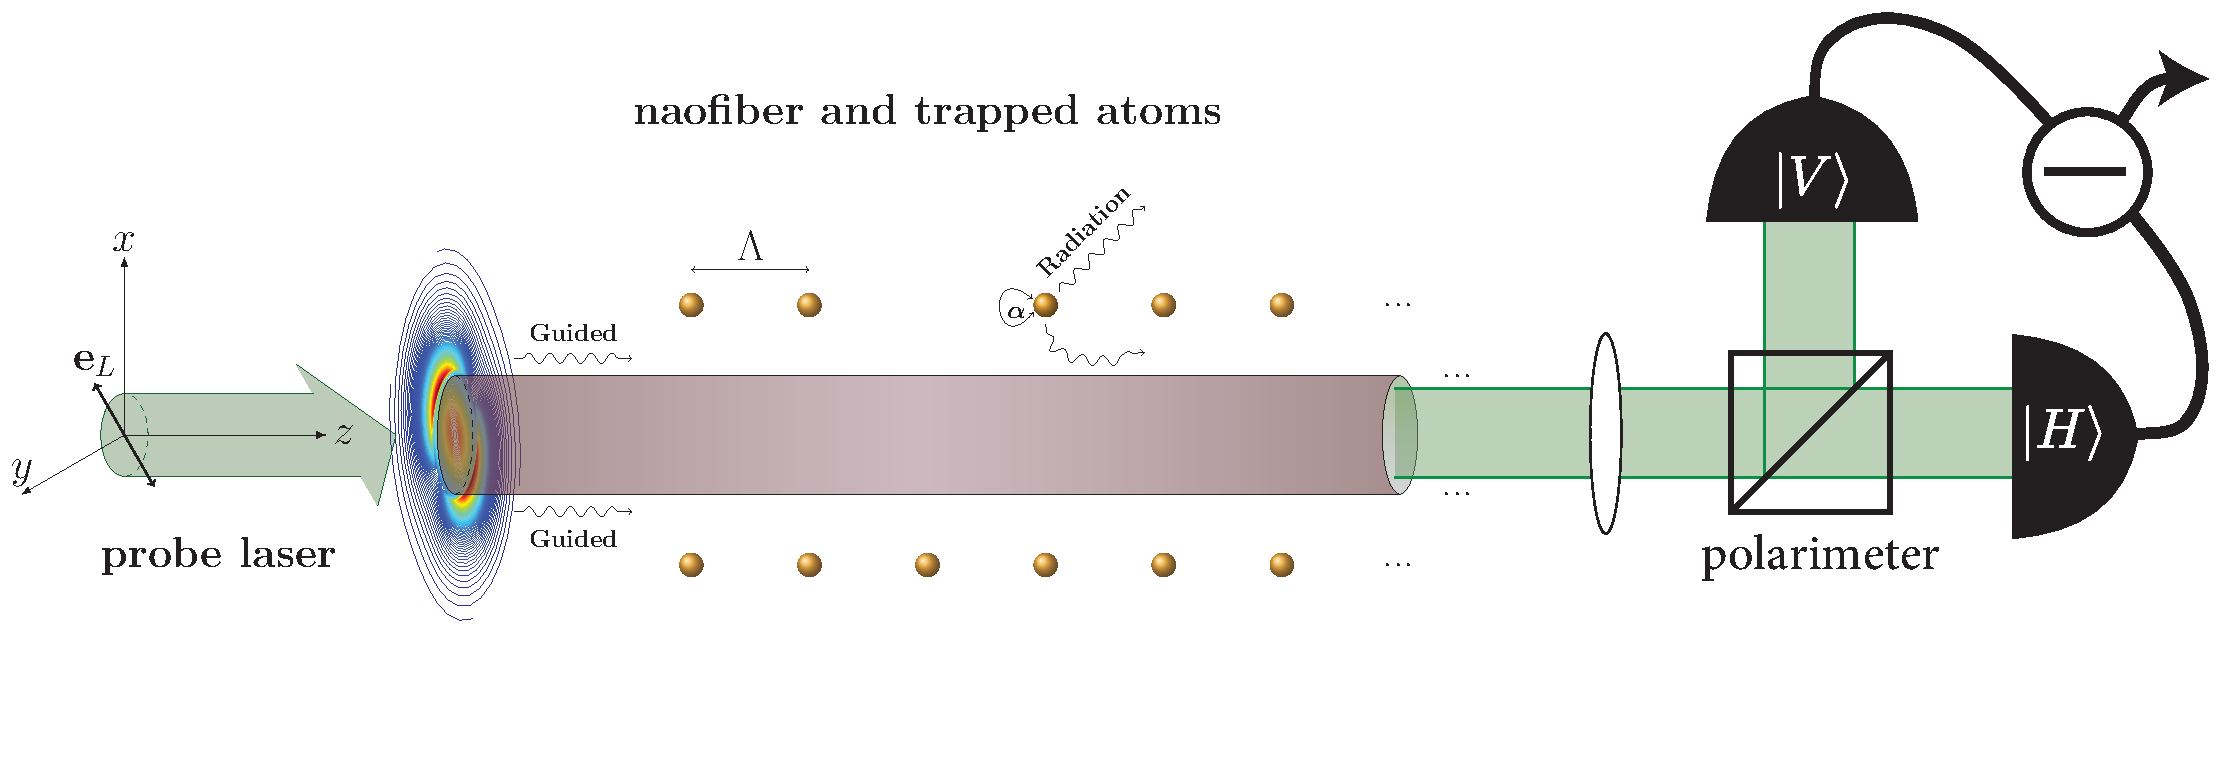
\includegraphics[scale=0.35]{./Figs/BirefringenceMeasurement_randomAtoms}
\caption{Birefringence measurement setup for a nanofiber trapped atomic system. In the evanescent 
field of the nanofiber, atoms (golden balls) randomly  occupy the periodic trapping sites on both sides of 
a 1D-chain with a period of $\Lambda$.}
\label{fig:BirefringenceMeasurement}
\end{figure}

%========GREEN'S FUNCTION AND INPUT/OUTPUT RESPONSE=========%
\section{Dyadic Green's function and input-output field response}

Given a point particle at position $\br'$ with tensor polarizability $\tensor{\boldsymbol{\alpha}}$, the total field  at frequency $\omega_0$ is given by the scattering solution to the wave equation, 
	\begin{align}\label{Eq::WaveEquationSource}
		\left[ - \nabla \times\nabla \times + n^2(\br)k_0^2 \right] \mathbf{E}(\br) &= -4\pi  k_0^2 \delta^{(3)}(\br-\br')\,  \tensor{\boldsymbol{\alpha}}\cdot \mathbf{E}(\br),
	\end{align}
where $k_0=\omega_0/c$ and $n(\mbf{r})$ is the spatially anisotropic index of refraction; Gaussian-cgs units are used throughout.  For an asymptotic input field $\mathbf{E}_{\inp}(\br)$, the scattering solution to \erf{Eq::WaveEquationSource} is given by the Lippmann-Schwinger equation \cite{wubs_multiple-scattering_2004},
	\begin{align}
		\mathbf{E}_{\out}(\br) &=\mathbf{E}_{\inp}(\br)+\tensor{\mathbf{G}}^{(+)}(\br , \br'; \omega_0)\cdot 
\tensor{\boldsymbol{\alpha}}\cdot \mathbf{E}_{\out}(\br')\\
		&\approx \mathbf{E}_{\inp}(\br)+ \tensor{\mathbf{G}}^{(+)}(\br , \br'; \omega_0) \cdot 
\tensor{\boldsymbol{\alpha}}\cdot \mathbf{E}_{\inp}(\br'), \label{Eq::ScatteredField}
	\end{align}
where in \erf{Eq::ScatteredField} we have made the first Born approximation valid for weak scattering. The fundamental object in that fully characterizes the scattered radiation as well as the energy level shift and modified decay rate of a scatterer near the dielectric is the (causal) dyadic Green's function, $\tensor{\mathbf{G}}(\br, \br';\omega_0)$, which satisfies
	\begin{align} \label{Eq::GreensDiffEq}
		\left[ -\nabla\times\nabla\times + n^2(\mbf{r}) k_0^2 \right] \tensor{\mathbf{G}}(\br, \br';\omega_0) &= -4\pi 
k_0^2 \delta^{(3)}(\mathbf{r}-\mathbf{r}') \unittens,
	\end{align}
with $\unittens$ being the unit tensor.  The imaginary part of the Green's function determines the Purcell effect on resonance \cite{}.  We seek here the off-resonance, dispersive response.  

A solution for the Green's function $\tensor{\mathbf{G}}(\br ,\br' ; \omega_0)$ following from Maxwell's equations 
has been studied previously \cite{sakoda_optical_1996,sondergaard_general_2001,wubs_multiple-scattering_2004}.  As we are interested here in the forward-scattered components that lead to phase shifts and polarization transformations, we directly calculate $\tensor{\mathbf{G}}(\br ,\br' ; \omega_0)$ through a decomposition into normal modes.  A complete set of eigenmodes in the presence of lossless, anisotropic dielectric are defined according to the procedure of Glauber and Lewenstein~\cite{glauber_quantum_1991}.  We seek the eigenmodes $\eigenf(\mathbf{r})$, with mode labels $\fidx$, that satisfy the homogeneous wave equation in the absence of sources, i.e. \erf{Eq::WaveEquationSource} for $\tensor{\boldsymbol{\alpha}} = 0$.  They are constructed by introducing the related functions, $\eigeng(\mbf{r}) \equiv n(\br) \eigenf(\mbf{r})$.  These functions form a complete set of vector functions, as they are eigenfunctions of the Hermitian operator, $\mathcal{H}(k_0) = -\frac{1}{n(\br)} \nabla\times\nabla\times \frac{1}{n(\br)} + k_0^2$, according to $\mathcal{H}(k_0)  \eigeng(\mbf{r}) = \lambda_\fidx \eigeng(\mbf{r})$. The eigenvalue, $\lambda_\fidx= k_0^2-k_\fidx^2$, determines the wavenumber for a given mode, $k_\fidx$.  We are interested specifically in the transverse functions, $\nabla \cdot \eigeng(\br) = 0$, with eigenvalues $\lambda_n \neq 0$.  These fall into two categories \comment{(what about the ``whispering gallery" modes?)}.  Modes whose transverse wavevector is purely imaginary outside the dielectric are guided, while the radiation (unguided) modes do not have this restriction. Together, the guided and radiation modes form a complete, orthonormal set for transverse vector functions:
	\begin{align}
	\int \mathrm{d}^3\br \, \eigeng^*(\mbf{r}) \cdot \eigengp(\mbf{r})  &= \int \mathrm{d}^3\br \, n^2(\br) \eigenf^* (\br)\cdot  \eigenfp(\br) =\delta_{\fidx, \fidx'},\label{Eq::Orthogonality}\\
	\sum_\fidx \eigeng(\br) \eigeng^*(\br') &= \sum_\fidx n(\br)n(\br') \eigenf(\br) \eigenf^*(\br') =\tensor{\delta}^{(T)}(\br-\br')  \unittens, \label{Eq::Completeness}
	\end{align}
where $\tensor{\delta}^{(T)}(\br-\br')$ is the delta function for transverse vector fields.  When the eigenfunctions form a continuous set, the sum over $\fidx$ in \erf{Eq::Completeness} represents an integral and likewise the discrete Kroenecker delta function in \erf{Eq::Orthogonality} represents a Dirac delta function.  It follows that the transverse dyadic Green's function can be decomposed in terms of the eigenfunctions~\cite{sakoda_optical_1996, sondergaard_general_2001}
	\begin{align}
		\tensor{\mathbf{G}}^{(T)}(\br,\br'; \omega_0)%& = -4\pi k_0^2 \sum_{\fidx} \frac{ n(\br) n(\br') \eigenf (\br) 
%\eigenf^* (\br')}{\lambda_\fidx}, \\
	&= -4\pi \sum_{\fidx} \frac{  \omega_0^2 \eigenf (\br) 
\eigenfp^* (\br')}{\omega_0^2-\omega_\fidx^2},
	\end{align}
where the eigenvalues appear as $\omega_\fidx^2 = c^2 k_\fidx^2$.  The sum includes both guided and unguided (radiation) contributions. We focus here on the guided-mode contribution to the Green's function. Details concerning the radiation modes of a nanofiber can be found in Refs. \cite{Snyder and Love, sondergaard_general_2001,le_kien_spontaneous_2005}.

We treat here an optical nanofiber of radius $a$ with step-index profile,
	\begin{align} \label{Eq::IndexofRefraction}
		n(r_\perp) = \Bigg\{  
			\begin{array}{l l} n_1 & \quad r \leq a \\
						 n_2 & \quad r > a 
		\end{array},
	\end{align}
for a silica core ($n_1 = 1.45$) and infinite vacuum cladding ($n_2 = 1$).  For a cylindrically symmetric dielectric the guided modes are $\eigenf (\br) = (2\pi)^{-1/2} \mathbf{u}_\mu (\br_\perp) e^{i\beta z}$, with indices $\mu=\{n, \beta, p\}$ for guided mode $n$ with propagation constant $\beta$ and polarization $p$.  The transverse mode functions are normalized according to $\int d^2 \mbf{r}_\perp \, n^2(r_\perp)\mathbf{u}^*_\mu (\br_\perp) \cdot \mathbf{u}_{\mu'} (\br_\perp)\big|_{\beta = \beta'} = \delta_{n,n'}\delta_{p,p'}$ and have units $1/\sqrt{A}$ \cite{le_kien_anisotropy_2014}.  Two convenient guided-mode bases are the quasilinear and quasicircular modes, given in  Appendix \ref{Appendix::ModeFunctions}, whose $z$-components satisfy the two-dimensional Schr\"{o}dinger-like equation, $\big[\nabla_\perp^2 +k_0^2 n^2(r_\perp) \big] u_{\mu,z} (\br_\perp) = \beta^2 u_{\mu,z} (\br_\perp)$ \cite{kien_field_2004}.  

The nanofiber supports only the lowest HE$_{11}$ guided modes \cite{Yariv} at the relevant frequency $\omega_0$, and thus we drop the mode index $n$.  In this case there are four guided modes: two polarizations $p$, each with propagation constant (longitudinal wavenumber) $\beta(\omega_0) = \pm\beta_0$ corresponding to forward and backward propagation.  The value of $\beta_0$ is found by enforcing the boundary conditions at the fiber surface and solving the eigenvalue equation \cite{Yariv, Marcuse, SnyderLove}. The guided-mode contribution to the dyadic Greens function is then 
	\begin{equation} \label{Eq::GreensEigenmodes}
		\tensor{\mathbf{G}}_g(\br,\br'; \omega_0) = \int_{-\infty}^\infty \frac{d \beta}{2 \pi} \sum_{p} 
\frac{-4\pi\omega_0^2}{\omega_0^2-\omega^2(\beta)} \mathbf{u}_{\beta,p} (\br_\perp)\mathbf{u}^*_{\beta,p} 
(\br_{\perp}^\prime) e^{i\beta(z-z')},
	\end{equation}
where $ \omega(\beta)$ is the frequency of the guided HE$_{11}$ for a given $\beta$.  The 
HE$_{11}$ mode has no cutoff; for a given $\omega$, there always exists a guided mode with propagation 
constant $\beta(\omega)$.  

For $z>z'$ ($z'>z$), the contribution of the guided modes to the retarded Green's function is found by the 
usual displacement of the pole on the positive (negative) $\beta$-axis into the upper (lower) half of 
the complex plane. Closing the contour yields \cite{manga_rao_single_2007}
	\begin{align} 
		\tensor{\mathbf{G}}^{(+)}_g(\br,\br'; \omega_0) = &2\pi i \sum_{f,p}  {\rm Res}\vert_{\beta =f\beta_0} 
\left[\frac{-4\pi \omega_0^2 }{2\pi ( \omega_0^2-\omega^2(\beta))}\right]  \mathbf{u}_{f\beta_0, p} 
(\br_\perp)\mathbf{u}^*_{f\beta_0, p} (\br_{\perp}^\prime)e^{if \beta_0 (z-z')} \nonumber \\
%&  =  i 2\pi f \frac{\omega_0}{v_g } \sum_{p} \mathbf{u}_{f, p} (\br\!_\perp)\mathbf{u}^*_{f , p} 
%(\br_{\!\perp}^\prime) e^{if \beta_0(z-z')}\;\; {\rm for }\;  (z-z')f>0,
%= & 2\pi i \frac{\omega_0}{v_g } \sum_{p} \Big[ \mathbf{u}_{+, p} (\br_\perp)\mathbf{u}^*_{+ , p} 
%(\br_{\!\perp}^\prime) e^{i\beta_0(z-z')} \Theta (z-z' ) \label{Eq::GreensGuided}\\
%	& \quad \quad \quad \quad \error{-} \mathbf{u}_{-, p} (\br_\perp)\mathbf{u}^*_{- , p} 
%(\br_{\perp}^\prime) e^{-i\beta_0(z-z')} \Theta  (z'-z)  \Big]  \nonumber \\
= & 2\pi i \frac{\omega_0}{v_g } \sum_{f,p} \mathbf{u}_{f, p} (\br_\perp)\mathbf{u}^*_{f , p} 
(\br_{\perp}^\prime) e^{i f \beta_0(z-z')} \Theta \big( (z-z')f \big), \quad \quad \error{(\mbf{r} \neq \mbf{r}')} \label{Eq::GreensGuided}
	\end{align}
where $f=\pm$ indicates the propagation direction, $v_g= \vert d\omega/d\beta \vert_{\beta=\beta_0}$ is the group velocity at $\omega_0$, and $\Theta \big( (z-z')f \big)$ is a Heaviside function enforcing causality for the forward- and backward-scattered fields. In the second line, we have suppressed the label $\beta_0$ as it is implicit in the definition of the guided modes at frequency $\omega_0$. 

Radiative properties of a scatterer, the decay rate and energy level shift, are determined by evaluation of the dyadic Green's function at the source point $\mbf{r} = \mbf{r}'$ \cite{fussell_decay_2005}.  However, for $z=z'$ we cannot close the contour. Instead, we expand the resonant denominator in \erf{Eq::GreensEigenmodes} with the poles moved to yield the retarded (causal) response,
\begin{equation}
\frac{1}{(\omega_0+i\epsilon)^2-\omega^2(\beta)}=\frac{1}{2 \omega(\beta)}\left[ \frac{1}{\omega_0+ i 
\epsilon - \omega(\beta)} - \frac{1}{\omega_0+ i \epsilon + \omega(\beta)} \right],
\end{equation}
 and employ the usual distribution identities \cite{sondergaard_general_2001},
\begin{equation}
\lim_{\epsilon \rightarrow 0_+} \frac{1}{\omega_0 + i \epsilon \mp 
\omega(\beta)}=\mathcal{P}\left[\frac{1}{\omega \mp \omega(\beta)} \right] + i \pi \delta (\omega_0 \mp 
\omega(\beta)).
\end{equation}
Only the positive-frequency component contributes to the $\delta$-function, and it follows that the imaginary part of the Green's function at $\br = \br'$ that determines the resonant ($\omega_0 = \omega_{eg}$) Purcell enhancement of spontaneous emission into the guided modes is \cite{dung_spontaneous_2000, fussell_decay_2005, chen_finite-element_2010}
	\begin{equation}
		\Im \big[\tensor{\mathbf{G}}^{(+)}_g(\br',\br'; \omega_{eg}) \big] = \pi \frac{\omega_{eg}}{v_g } \sum_{f, p} 
		\mathbf{u}_{f, p} (\br_{\!\perp}^\prime)\mathbf{u}^*_{f , p} (\br_{\!\perp}^\prime).
	\end{equation}
The energy level shift of the scatterer due to its proximity to the dielectric is found from the real part of the Green's function at $\br = \br'$. The total modified spontaneous emission rate requires including the radiation modes \cite{le_kien_spontaneous_2005} or using other representations of the Green's function \cite{klimov_spontaneous_2004}.  

We note here that in a careful derivation of the Lippman-Schwinger scattering equation, it is not the total Green's function that appears in \erf{Eq::ScatteredField}, but rather a related dyadic quantity, $\mbf{K}(\br,\br', \omega_0) = \mbf{G}(\br,\br', \omega_0) + \delta(\br-\br')/n^2(\br)$ \cite{wubs_multiple-scattering_2004}. This function arises by properly accounting for the scatterer's coupling to the \emph{displacement} field rather than the electric field \cite{yao_ultrahigh_2009}.  The distinction becomes important at the source point $\mbf{r} = \mbf{r}'$; however, for lossless dielectrics $n(\mathbf{r})$ is real and $\Im[\tensor{\mathbf{G}}(\br',\br'; \omega)] = \Im[\tensor{\mathbf{K}}(\br',\br'; \omega)]$ \cite{yao_-chip_2010}. 

Equation (\ref{Eq::GreensGuided}) is the central result from which we can calculate the dispersive response.  Consider a forward-propagating ($f=+$) input field in the guided modes with frequency $\omega_0$ and arbitrary polarization, $\mathbf{E}^{(+)}_{\inp}(\br) = \mathcal{E}^{(+)}_0 (2\pi)^{-1/2} \mathbf{u}_{\rm in}(\br_\perp) e^{i \beta_0 z}$ with peak positive-frequency amplitude $\mathcal{E}_0$. The field has been expanded in the transverse mode functions,
	\begin{align} \label{Eq::uin}
		\mbf{u}_{\rm in}(\mbf{r}_\perp) = \sum_{p} c_{p} \mathbf{u}_{\fwd,p}(\br_\perp),
	\end{align}
with expansion coefficients satisfying $\sum_{p} |c_{p}|^2 = 1$.  The effective mode area at the atom's position is determined from the total cycle-averaged power transported along the nanofiber, $P_{{\rm in},z} = (v_g/8\pi) |\mathcal{E}^{(+)}|^2$, and the intensity at the atom, $I_{\rm in}(\mathbf{r}') = (c/8\pi)|\mathcal{E}^{(+)}|^2|\mbf{u}_{\rm in}(\mbf{r}_\perp')|^2$, via the relation \cite{domokos_quantum_2002},
 	\begin{align} \label{Eq::AreaIn}
 		A_{\rm in} \equiv \frac{P_{{\rm in}}}{I_{\rm in}(\mathbf{r}')} = \frac{1}{n_g |\mathbf{u}_{\rm in}(\mathbf{r}'_\perp)|^{2}}.
	\end{align}
Tight confinement of the guided modes in the nanofiber results in significant intensity near the nanofiber for relatively small input power \cite{bures_power_1999}.  Note that $P_{\rm in}$ is not the total power, as some of the energy is transported around the nanofiber azimuthally due to the longitudinal component of the guided modes \cite{le_kien_scattering_2006}.

Substitution of the guided-mode Green's function, \erf{Eq::GreensGuided}, into the Lippman-Schwinger equation, \erf{Eq::ScatteredField}, yields the transmitted (forward-scattered) and reflected (backward-scattered) output fields, $\mathbf{E}_{\out}(\br) = \mathcal{E}_0 (2\pi)^{-1/2} \big[ \mathbf{u}_{\trans, \out} (\br_\perp) e^{i \beta_0 z} + \mathbf{u}_{\refl,\out} (\br_\perp) e^{-i \beta_0 z} \big]$, 
	\begin{align}
		\mathbf{u}_{\trans, \out} (\br_\perp) &=  \sum_{p,p'}  \, c_{p} t_{pp'} \mathbf{u}_{\fwd, p'}(\br_\perp) \\ 
		\mathbf{u}_{\refl,\out} (\br_\perp) &=  \sum_{p,p'}  \, c_{p} r_{pp'} \mathbf{u}_{\bwd, p'}(\br_\perp). 
	\end{align}
For an atom located at $\br'$, the transmission and reflection matrices are 
	\begin{align} \label{Eq::PolarizationTransformation}
		t_{pp'} =& \delta_{p,p'} + i 2\pi k_0 n_g \, \mathbf{u}^*_{+, p'}(\br'_\perp) \cdot 
\tensor{\boldsymbol{\alpha}} \cdot \mathbf{u}_{+, p}(\br'_\perp) \Theta ( z-z' ) , \\
		r_{pp'} =& i 2\pi k_0 n_g \, \mathbf{u}^*_{\bwd, p'}(\br'_\perp) \cdot 
\tensor{\boldsymbol{\alpha}} \cdot \mathbf{u}_{\fwd, p}(\br'_\perp) e^{2 i\beta_0 z'} \Theta ( z'-z ) , 
	\end{align} 
where $n_g = c/v_g$ is the group index of refraction.  We focus here on the transmitted fields whose interference with the input field for $z>z'$ results in a phase shift and polarization transformation.  For weak scattering the diagonal terms, $t_{p p} \approx \sqrt{1-R_p}e^{i \delta \phi_p}$, determine the phase shift and attenuation induced on each polarization:
	\begin{align}
		\delta \phi_p &= \frac{2 \pi k_0}{A_{\rm in}} \frac{\Re(\alpha_{pp})}{|\mathbf{u}_{\rm in}(\mathbf{r}'_\perp)|^{2}} , \label{Eq::PhaseShift} \\
		R_p &=  \frac{4 \pi k_0}{A_{\rm in}}\frac{\Im(\alpha_{pp})}{|\mathbf{u}_{\rm in}(\mathbf{r}'_\perp)|^{2}} , \label{Eq::Attenuation}
	\end{align}
where the $\{p,p'\}$-element of the tensor polarizability is given by 
	\begin{align} \label{Eq::PolarizabilityElementsClassical}
		\change{\alpha_{pp'} \equiv \mathbf{u}^*_{+,p'}(\br'_\perp) \cdot \tensor{\boldsymbol{\alpha}}\cdot \mathbf{u}_{+, p}(\br'_\perp). }
	\end{align} 
\comment{I think we should take out the mode functions and instead use the normalized polarization vectors, $\mathbf{e}_p = \mathbf{u}_{+,p'}(\br'_\perp)/|\mathbf{u}_{+,p'}(\br'_\perp)|$. Then, this equation is \emph{actually} the $\{p,p'\}$-element of the tensor polarizability and the effective area has been entirely factored out,
	\begin{align}
		\delta \phi_p &= \frac{2 \pi k_0}{A_{\rm in}} \Re(\alpha_{pp}),  \\
		R_p &=  \frac{4 \pi k_0}{A_{\rm in}} \Im(\alpha_{pp}) .
	  \end{align} 
}

The phase shift per atom, \erf{Eq::PhaseShift}, is modified over free space in two ways which are both captured by the effective mode area $A_{\rm in}$.  First, due to the tight spatial confinement of the guided mode, trapped atoms experience fields orders of magnitude larger than in free space.  Further, diffraction in free space limits the number of atoms that can be present in the areas of highest electric field near the focus \cite{baragiola_three-dimensional_2014}.  Second, although material dispersion in an optical fiber is negligible, a dielectric with a small effective mode area can have significant waveguide dispersion. The dispersion relation $\omega(\beta)$ near $\beta_0$ can lead to enhanced atom-light coupling from a reduction in the group velocity. In the nanofiber geometry, this factor leads to a small improvement, \comment{ $n_g \approx 1.4$. Figure showing effective mode areas and group velocities?}
 
The off-diagonal terms in the transmission matrix correspond to polarization transformations.  For example, if we take the polarizations to be the quasilinear modes ($p = H,V$) given in \erf{Eq::QuasilinearModes}, then $t_{HV} \equiv \chi_{\rm Far}$ \comment{(check factors of 2)}, the rotation angle of the Faraday effect \cite{}.  In this basis, the phase difference $\delta  \phi_H - \delta \phi_V$ corresponds to birefringence.  Alternatively, analyzed in the quasicircular modes ($p=\pm$) given in \erf{Eq::QuasicircularModes}, $\delta \phi_+ -\delta  \phi_-$ corresponds to Faraday rotation and $t_{+-}$ to birefringence.  We make use of such polarization transformations as a means to nondestructively measure the atoms and generate collective spin squeezing.

\comment{How does our scattering matrix relate to that from Le Kien's results about propagation of light through an array of nanofiber-trapped atoms?  Specifically, Eq. (8) of Ref. \cite{le_kien_correlations_2008} and/or Eqs. (8-10) of Ref. \cite{le_kien_propagation_2014}?  
}
	
	%===================Heisenberg-Langevin Equations=====================%
	\subsection{Heisenberg-Langevin-picture solution and atomic response}
	
The Lippmann-Schwinger solution, \erf{Eq::ScatteredField}, determines the input-output relation for linear atomic response given by the polarizability tensor $\tensor{\alpha}$.  In this section we derive the fully quantum mechanical description of dispersive atomic response and input-output relations for the quantized guided modes.  Following closely Ref. \cite{le_kien_spontaneous_2005}, we use a Heisenberg-Langevin approach for one-dimensional systems.  

The positive frequency component of the quantized electric field operator decomposes into guided and radiation (unguided) modes, $\hat{\mathbf{E}}^{(+)}=\hat{\mathbf{E}}_g^{(+)}+\hat{\mathbf{E}}_{r}^{(+)}$, where
	\begin{align}
		\hat{\mathbf{E}}_g^{(+)}(\br) &= \sum_{f,p} \int \mathrm{d}\omega  \sqrt{\frac{ \hbar \omega}{ v_g}} \awg \mathbf{u}_\mu (\br\!_\perp) e^{i f\beta(\omega) z } ,\label{Eq::QuantizedElectricField} \\
		\hat{\mathbf{E}}_r^{(+)}(\br) &= \sum_{m,p} \int \mathrm{d}\omega   \int_{-kn_2}^{kn_2}\mathrm{d}\beta \, \sqrt{ \hbar \omega}\awr \mathbf{u}_\nu (\br\!_\perp) e^{i\beta(\omega) z },
	\end{align}
The four HE$_{11}$ guided modes are indexed by $\mu =(\omega, f, p)$ for two polarizations $p$ and two propagation directions $f=\pm1$ with wavenumbers $f\beta (\omega)$.  The radiation modes are indexed by  $\nu=(\omega, \beta, m, p)$ where $\omega$ is the frequency, $m$ is the azimuthal quantum number (angular momentum), $p$ labels the two orthogonal polarizations. The longitudinal propagation constant $\beta(\omega)$ can vary from $-kn_2$ to $kn_2$, with $k = \omega/c$ \cite{sondergaard_general_2001,le_kien_spontaneous_2005}.  The creation/annihilation operators satisfy the usual continuous-mode commutation relations, $[\hat{a}_\mu, \hat{a}^\dag_{\mu'} ] = \delta_{f,f'} \delta_{p,p'} \delta ( \omega - \omega ') $, $[\hat{a}_\nu ,\hat{a}^\dag_{\nu'} ] = \delta_{m,m'} \delta_{p,p'} \delta ( \omega - \omega ')  \delta ( \beta - \beta') $.

The Hamiltonian for the system is
\begin{equation}
\hat{H} = \hat{H}_F+\hat{H}_A + \hat{H}_{\inter}.
\end{equation}
The free field Hamiltonian decomposes into guided and unguided modes, 
	\begin{equation}
		\hat{H}_F = \sum_{f,p}\int \mathrm{d}\omega \, \hbar \omega \hat{a}^\dagger_\mu \hat{a}_\mu 
+\sum_{m,p} \int \mathrm{d}\omega  \int_{-k n_2}^{k n_2} \mathrm{d}\beta \, \hbar \omega 
\hat{a}^\dagger_\nu \hat{a}_\nu.
	\end{equation}
We consider here alkali atoms with hyperfine multiplets of ground and excited levels, $\{ 
\ket{g}=\ket{nS_{1/2}, F, M_F}\}$, $\{ \ket{e} =\ket{nP_{J'}, F', M_{F'}}\}$,
	\begin{equation}
		\hat{H}_A  = \sum_g E_g \hat{\sigma}_{gg} + \sum_e E_e \hat{\sigma}_{ee},
	\end{equation}
with atomic transition operators $\hat{\sigma}_{ij} \equiv \ket{i}\bra{j}$.  In the rotating wave approximation, the atom-field interaction Hamiltonian is
	\begin{align}
		\hat{H}_{\inter} &= -\hat{\mathbf{d}}\cdot \hat{\mathbf{E}} = -\hat{\mathbf{d}}_{eg}\cdot 
\hat{\mathbf{E}}^{(+)}(\br')-\hat{\mathbf{d}}_{ge}\cdot \hat{\mathbf{E}}^{(-)}(\br'),
	\end{align}
where the atomic dipole operator is projected between excited and ground subspaces, $\hat{\mathbf{d}}_{eg}= \hat{P}_e \hat{\mathbf{d}} \hat{P}_g $. The interaction Hamiltonian then takes the form, 
\begin{equation}
	\hat{H}_{\inter} = -\sum_{e,g} \left(\sum_{f,p} \int\mathrm{d}\omega \; \hbar g_{\mu, e,g}\, \hat{a}_\mu  \, 
		\hat{\sigma}_{eg}+ \sum_{m,p} \int\mathrm{d}\omega \! \int_{-kn_2}^{kn_2}\mathrm{d}\beta \,  \hbar 
g_{\nu, e,g}\, \hat{a}_\nu \, \hat{\sigma}_{eg}\right) + {H.c.},
	\end{equation}
where the coupling constants between the electric dipole and the guided/radiation modes are
\begin{subequations} \label{Eq::CouplingConstants}
	\begin{align}
		\hbar g_{\mu, e,g} &= \sqrt{\frac{\hbar \omega}{ v_g  }}\, \bra{e} \hat{\mathbf{d}} \ket{g} 
\cdot\mathbf{u}_\mu (\br') e^{i f \beta(\omega)z} , \\
		\hbar g_{\nu, e,g} &= \sqrt{  \hbar \omega } \, \bra{e} \hat{\mathbf{d}} \ket{g} \cdot \mathbf{u}_\nu (\br') e^{i\beta(\omega)z}  .
\end{align}
	\end{subequations}
The Heisenberg equations of motion thus follow,
	\begin{align}
		\der{\hat{a}_\mu} &= -i\omega \hat{a}_\mu +i\sum_{e,g} g_{\mu, e,g}^* \hat{\sigma}_{ge} \label{eq:da}\\
		\der{\hat{a}_\nu} &= -i\omega \hat{a}_\nu +i\sum_{e,g} g_{\nu, e,g}^*  \hat{\sigma}_{ge}\label{eq:danu}\\
		\der{\hat{\sigma}_{ge}} &= -i\omega_{eg} \hat{\sigma}_{ge} \label{Eq::dsigma}  \\
			&+ i\int_0^{\infty}\mathrm{d}\omega \sum_{e',g'} \bigg[ \big(\delta_{ee'} \hat{\sigma}_{gg'} - \delta_{gg'} \hat{\sigma}_{e'e} \big) \bigg\{ \sum_{f,p}  g_{\mu, e',g'}\hat{a}_\mu (\omega; t) +\sum_{m,p} \int_{-kn_2}^{kn_2}\mathrm{d}\beta \; g_{\nu, e',g'} \hat{a}_\nu(\omega, \beta; t) \bigg\} \bigg]. \nonumber
	\end{align}
Integrating the field equations, 
\begin{subequations}\label{eq:aout1}
\begin{align}
\hat{a}_\mu(\omega, t) &= \hat{a}_\mu(\omega; t_0) e^{-i\omega (t-t_0)} +i \sum_{e,g} g_{\mu,e,g}^* \int_{t_0}^t 
\mathrm{d} t' e^{-i\omega (t-t')}\hat{\sigma}_{ge}(t') \label{Eq::aguidedEOM}
\end{align}
\begin{align}
\hat{a}_\nu (\omega; t) &= \hat{a}_\nu (\omega; t_0) e^{-i\omega (t-t_0)} +i \sum_{e,g} g_{\nu,e,g}^* \int_{t_0}^t \mathrm{d} 
t' e^{-i\omega (t-t')}\hat{\sigma}_{ge}(t'),
\end{align}
\end{subequations}
substituting into \erf{Eq::dsigma}, and making the usual Markov approximation~\cite{?} gives an expression for the ground-excited state coherences,
\begin{align}
&\dt{\hat{\sigma}_{ge}} =-i\omega_{eg} 
\hat{\sigma}_{ge}-\sum_{e'}\frac{\Gamma_{ee'}}{2}\hat{\sigma}_{ge'}  \\
&+i \sum_{e',g'}\bigg[ (\delta_{e,e'} \hat{\sigma}_{gg'} - \delta_{g,g'} 
\hat{\sigma}_{e'e})\int_0^{\infty}\mathrm{d}\omega \bigg\{\sum_{f,p}  g_{\mu, e',g'} \hat{a}_\mu (t_0) 
+\sum_{m,p}  \int_{-kn_2}^{kn_2}\mathrm{d}\beta  g_{\nu, e',g'} \hat{a}_\nu(t_0) \bigg\} e^{-i\omega 
(t-t_0)}\bigg], \nonumber
\end{align}
where the decay of excited-state correlations is given by 
	\begin{equation}
		\Gamma_{ee'} = 2\pi \sum_{\mu,g} g_{\mu,e,g}g^*_{\mu,e',g} \vert_{\omega=\omega_{eg}}+2\pi 
\sum_{m,p,g} \int d\beta \, g_{\nu,e,g}g^*_{\nu,e',g} \vert_{\omega=\omega_{eg}}, \label{Eq::TotaleeDecayRate}
	\end{equation}
and the small energy shift is absorbed into the transition frequency $\omega_{eg} = (E_e - E_g)/\hbar$.  Equation (\ref{Eq::TotaleeDecayRate}) captures the modification of the spontaneous emission rate due to the nanofiber, which alters the local density of states \cite{le_kien_spontaneous_2005}.  The first sum describes decay into the guided modes and the second into the unguided radiation modes \cite{ nha_cavity_1997,klimov_spontaneous_2004,le_kien_spontaneous_2005,maslov_distribution_2006}. The decay rate of a given excited state into all the guided modes is given by
	\begin{equation}
		\Gamma_e^{\oneD}= 2\pi \sum_{\mu,g} |g_{\mu,e,g} |^2_{\omega = \omega_{eg}} =  \frac{ 2\pi }{\hbar} \frac{ \comment{\omega_{eg}} }{v_g} \sum_{\mu,g} \big|\bra{e}\hat{\mathbf{d}}\ket{g} \cdot \mathbf{u}_{fp}(\br'_\perp)\big|^2  .
	\end{equation}
This agrees with the expected expression following from the guided-mode contribution to the dyadic Green's function, \erf{Eq::GreensGuided},
	\begin{equation}
		\Gamma_e^{\oneD} =  \frac{2}{\hbar} \sum_{g}  \bra{g}\hat{\mathbf{d}}\ket{e}\cdot 
\Im \Big[\tensor{\mathbf{G}}^{(+)}_g(\br', \br'; \omega_{eg} ) \big] \cdot \bra{e}\hat{\mathbf{d}}\ket{g} ,
	\end{equation}
enhanced over the free-space rate by the Purcell factor.  In general, the decay rate into a given mode depends on the dipole orientation \cite{klimov_spontaneous_2004, vos_orientation-dependent_2009}. Recently, it was predicted \cite{le_kien_anisotropy_2014} and demonstrated \cite{mitsch_quantum_2014} that the decay rates into the forward and backward modes are not always equal.  Specifically, when the atomic dipole has a component rotating in the plane defined by the atom and nanofiber, the relative decay rates can differ due to the longitudinal component of the guided modes. \comment{Maybe we should include a plot of $\Gamma_{\rm 1D}/\Gamma_0$.  This is the \emph{first} thing people ask.  We must make the point that while it's not so large, we can benefit from many atoms much more easily than other systems, such as those alligator waveguide photonic crystals.}

Here we are interested in linear response for excitation far from resonance.  We follow Ref. \cite{le_kien_propagation_2014} and consider an atom sufficiently far from the fiber surface such that the modification of the spontaneous emission rate is small.   In this case the decay rate is approximated as $\Gamma_{ee'} \approx \delta_{e,e'} \Gamma_{e}$, where $\Gamma_e$ is the total decay rate from excited state $\ket{e}$, given by the diagonal elements of \erf{Eq::TotaleeDecayRate}.  In steady state, the dipole operator in the linear regime ($\hat{\sigma}_{ee'} \rightarrow 0 $) is approximately
	\begin{align}
		\hat{\sigma}_{ge} \approx -\sum_{g'} \hat{\sigma}_{gg'}\int_0^{\infty}\mathrm{d}\omega \bigg( & \sum_{f,p}  
\frac{g_{\mu, e,g'}}{\omega-\omega_{eg} \error{+} i \Gamma_{e}/2  }\, \hat{a}_\mu (t_0) \\
	&+\sum_{m,p} \int_{-kn_2}^{kn_2}\mathrm{d}\beta \, \frac{g_{\nu, e,g'}}{\omega-\omega_{eg} \error{+} i \Gamma_{e}/2 } \,\hat{a}_\nu (t_0)  \bigg)e^{-i\omega (t-t_0)} , \nn
	\end{align}
By substituting this into \erf{Eq::aguidedEOM} and defining asymptotic modes, \comment{ $\hat{a}^{\inp}(\omega) = \lim_{t_0\rightarrow -\infty} \hat{a}(t_0) e^{i\omega t_0}$, $\hat{a}^{\out}(\omega) = \lim_{t\rightarrow +\infty} \hat{a}(t) e^{i\omega t}$ \cite{fan_input-output_2010}}, we obtain the input-output relationship for the guided modes,
	\begin{equation} \label{Eq::aout}
		\hat{a}^{\out}_\mu (\omega) = \hat{a}^{\inp}_\mu (\omega) \!-\! 2\pi i\sum_{p',f'} 
\sum_{e,g,g'}\!\hat{\sigma}_{gg'}\frac{ g_{\mu,e,g}^* g_{\mu',e,g'}}{ \Delta_{eg} \error{+} i \Gamma_{e}/2 }\hat{a}^{\inp}_{\mu'}(\omega) \!-\! 2\pi i\sum_{m,p} \sum_{e,g,g'} \int^{kn_2}_{-kn_2} d\beta \,\hat{\sigma}_{gg'}\frac{ g_{\mu,e,g}^* g_{\nu',e,g'}}{ \Delta_{eg} \error{+} i \Gamma_{e}/2 }\hat{a}^{\inp}_{\nu}(\omega),
	\end{equation}
where $\Delta_{eg} = \omega - \omega_{eg}$.  The real part this relationship describes the coherent elastic scattering of photons from all modes--guided and radiation--into guided mode $\mu$, mediated by the atomic state.  The imaginary part describes loss from incoherent spontaneous emission into other modes.  For low atomic saturation, elastic scattering dominates and the interaction is purely dispersive. 

Equation (\ref{Eq::aout}) agrees with the expected form given by the Lippmann-Schwinger equation in the first Born approximation,
	\begin{equation} \label{Eq::IOScatteredField}
		\hat{\mathbf{E}}^{(+)}_{\out,g}(\br)=\hat{\mathbf{E}}^{(+)}_{ \inp, g}(\br)+\tensor{\mathbf{G}}_g^{(+)}(\br,\br',\omega)\cdot \poltens \cdot \Big[\hat{\mathbf{E}}^{(+)}_{\inp, g}(\br')+\hat{\mathbf{E}}^{(+)}_{\inp,r}(\br') \Big],
	\end{equation}
by noting
	\begin{equation}
		\int d^2 \mbf{r} \, \mathbf{u}^*_{\mu} (\br)\cdot \tensor{\mathbf{G}}_g^{(+)}(\br,\br',\omega)\cdot 
\poltens \cdot \mathbf{u}_{\mu'} (\br') =  i \frac{ 2\pi \omega_0}{v_g} \mathbf{u}^*_\mu 
 (\br') \cdot \poltens \cdot \mathbf{u}_{\mu'} (\br') = - i \frac{2 \pi}{\hbar} \sum_{e,g,g'}\!\ 
 \hat{\sigma}_{gg'} \frac{g_{\mu,e,g}^* g_{\mu',e,g'}}{ \Delta_{eg} \error{+} i \Gamma_{e}/2 }, 
	\end{equation}
where the guided-mode dyadic Green's function is given in \erf{Eq::GreensGuided} and the atomic polarizability operator is \cite{buhmann_casimir-polder_2004, deutsch_quantum_2010,kien_dynamical_2013},
	\begin{equation} \label{Eq::PolarizabilityOperator}
		\poltens = - \frac{1}{\hbar} \sum_{e,g,g'}\ket{g}\frac{\bra{g}\hat{\mathbf{d}}\ket{e}\bra{e} 
\hat{\mathbf{d}}\ket{g'}}{\Delta_{eg}  \error{+} i \Gamma_{e}/2 }\bra{g'}.
	\end{equation}
	
Scattering of classical waves follows when the field is in a coherent state.  \comment{Explaining this well is of critical importance - while injection of a classical field does not change the Purcell effect or decay rate (which is tied to the atomic transition frequency) it does scatter into all field modes with the same frequency, thus promoting them from vacuum}.  The phase-shift on a guided mode with a given polarization $p$, \erf{Eq::PhaseShift}, now depends on the internal state of the atom.  Given an atom in a particular ground sublevel $\ket{g}$, this can be expressed \cite{le_kien_propagation_2014}
	\begin{equation} \label{Eq::PhaseShiftMultilevel}
		\delta  \phi_{p,g} =2\pi \frac{\comment{ \omega_{0}}}{v_g} \mathbf{u}^*_{+, p}(\br'_\perp) \cdot \Re \big[\bra{g} 
\hat{\tensor{\boldsymbol{\alpha}}} \ket{g} \big] \cdot \mathbf{u}_{+, p}(\br'_\perp) = -\frac{1}{\hbar} \sum_e \frac{ \comment{ \omega_{eg} } }{v_g} \frac{2 \pi |\bra{e}\hat{\mathbf{d}}\ket{g} \cdot \mathbf{u}_{+,p}(\br'_\perp)|^2}{ \Delta_{eg} } ,
	\end{equation}
where $\Delta_{eg} = \omega_0 - \omega_{eg}$ is the laser detuning from the atomic transition frequency.  For large detuning, $\Gamma_{e}/\Delta_{eg} \ll 1$, the scattering is entirely elastic.  In this case, the absorption/scattering loss can be ignored and \erf{Eq::PhaseShiftMultilevel} describes a pure dispersive phase shift.

\change{
In relation to \erf{Eq::PhaseShift} we see that $\delta \phi \propto (\sigma_0/A_{\rm in}) (\Gamma_{\oneD}/\Delta)$ for resonant scattering cross section $\sigma_0$ and effective mode area $A_\inp$. For comparison, the phase shift on a paraxial laser beam imparted by an atom in free space has the same form, with the $\mathrm{TEM}_{00}$ mode for a beam waist $w_0$ and mode area $A= \pi w_0^2/2$ replacing the guided mode at the atom's position  \cite{tanji-suzuki_chapter_2011, baragiola_three-dimensional_2014}. The strongest phase shift in free space is achieved when the atom is placed at the center of the beam waist where the intensity is largest. The relative strength of the phase shift is $\delta \phi_{\rm fiber}/\delta \phi_{\vac}\propto A/A_{\rm in}$, as plotted in Fig. \ref{} as a function of the radial position of the atom \comment{(Le Kien's recent paper only considered mixed states; specifically an equal distribution of population among the sublevels for which there was no polarization transformation, only phase shifts)}.  For example, for a quasilinear field, and an atom trapped along the direction of the input polarization  at $r_\perp = ?$, $\delta \phi_{\rm fiber}/\delta \phi_{\vac} = ?$.   Thus we see that, in the nanofiber geometry the Purcell factor does not cause the majority of scattering to be guided, nor is the phase shift enhanced greatly over the phase shift imparted by an atom at the center of a paraxial beam. However, the key feature is that for a chain of atoms trapped along the fiber, the phase shifts add linearly.  Thus, one can achieve large optical densities, OD$_{\rm eff} = N_A (\sigma_0/\Ain)$ \comment{Decide how to properly define OD}, in the fiber geometry with far fewer atoms ($\sim 1000$ atoms) than are required in free space (\error{ $\sim 10^6$ }).  The result is a much larger average entangling interaction \emph{per atom} whose application in QND measurement we explore in the following section.
}

\begin{figure}
\begin{minipage}{.49\linewidth}
\centering
\subfloat[]{\label{fig:RelEnhanceFactor_r_w10micro}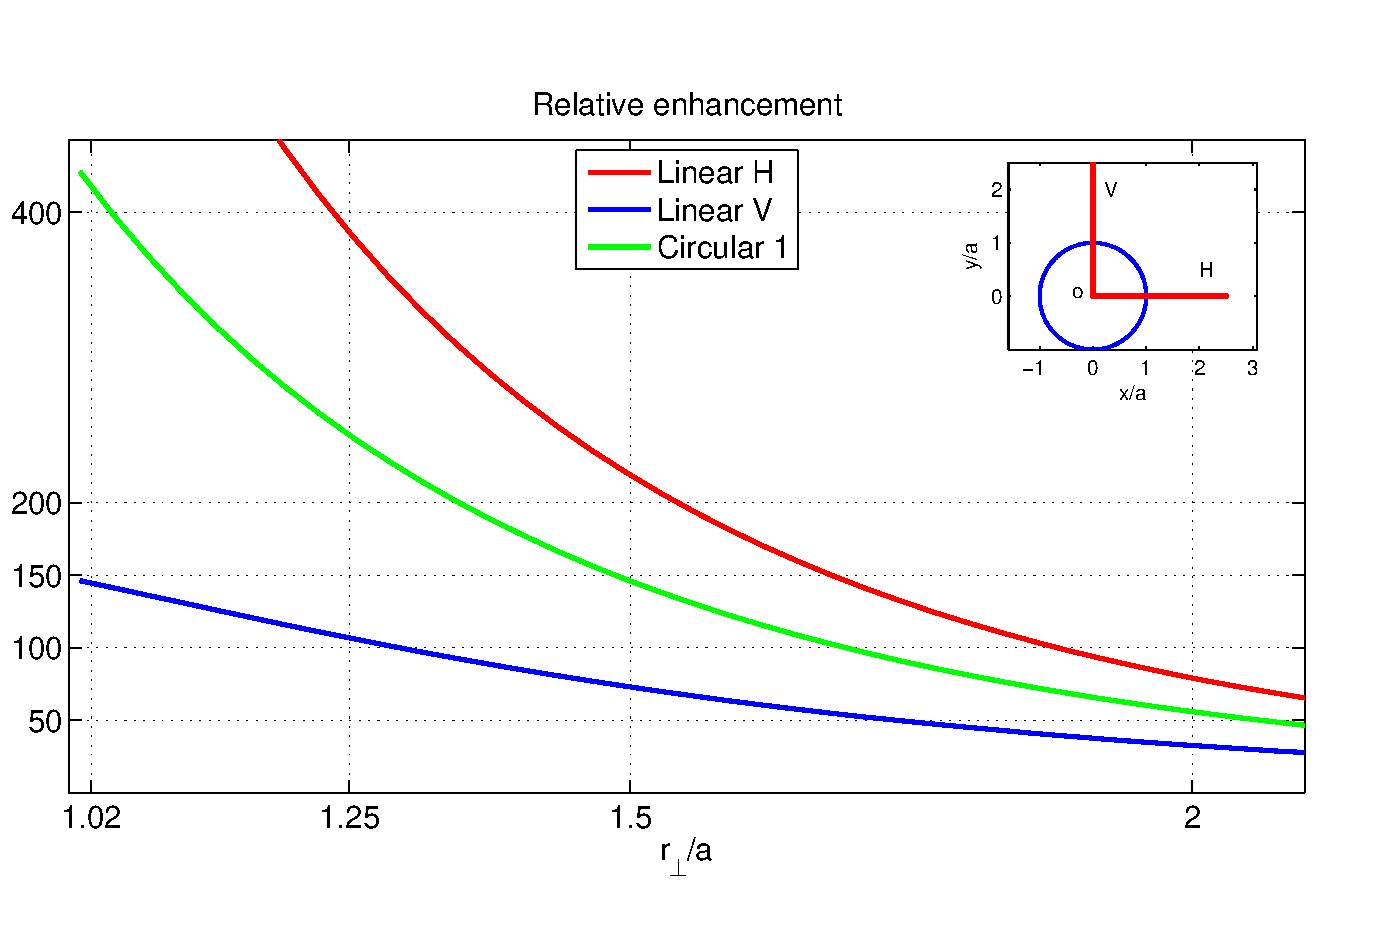
\includegraphics[scale=0.45]{./Figs/RelEnhanceFactor_r_w10micro}}
\end{minipage}
\caption{Subfigure~\protect\subref{fig:RelEnhanceFactor_r_w10micro} shows the relative enhancement factor of phase shift due to one atom in presence of a nanofiber as a function of the radial position of the atom. The enhancement factor is normalized to the phase shift when the atom was trapped at the center of a Gaussian beam with a waist of $ 10\,\mu m $. Quasilinearly and quasicircularly polarized fiber modes are used in this plot. \comment{Better to use an optimized free-space trapping configuration for comparison.}}\label{fig:modeparaperty}
\end{figure}


%===================QND Measurement=====================%
\section{QND measurement of atoms}
The dispersive interface between the atoms and nanofiber guided photons provides an entangling mechanism with which to perform a QND measurement on the atoms.  Linearly polarized probe light launched into the nanofiber adiabatically transforms through the fiber taper into a superposition over the guided modes, given in Appendix \ref{Appendix::ModeFunctions}.  Through the nanofiber-mediated dispersive interaction described above, which per atom is orders of magnitude stronger than in free space, the forward-scattered light undergoes a polarization transformation that encodes the atom-light entanglement \cite{geremia_tensor_2006, deutsch_quantum_2010,hammerer_quantum_2010}.  Continuous polarimetry of the scattered light performs a quantum nondemolition (QND) measurement of the collective atomic spin \cite{chaudhury_continuous_2006}, which can be used for a variety of quantum information processing tasks including nondestructive atom-number measurements \cite{dawkins_dispersive_2011, beguin_generation_2014}, state tomography \cite{smith_quantum_2013} and generation of entangled spin-squeezed states \cite{kuzmich_generation_2000, takano_spin_2009} for enhanced quantum sensing \cite{sewell_magnetic_2012}. 

We restrict here to the quasilinear modes, $p =\{H,V\}$, of a single HE$_{11}$ guided mode at frequency $\omega_0$, whose form is given explicitly in \erf{Eq::QuasilinearModes}.  In experimental configurations, two one-dimensional arrays of atoms are trapped on either side of the nanofiber, see Fig. \ref{}. The plane established by the atoms defines the quasi-$H$ ($\phi = 0$) and quasi-$V$ ($\phi = \pi/2$) axes. In the nanofiber region, the $H$-mode is purely $x$-polarized at $\phi = \pm \pi/2$ and the $V$-mode is purely $y$-polarized at $\phi = \{0,\pi\}$.  At other azimuthal angles the electric field is generally rotating along an ellipse.  The atoms trapped along the $x$-axis at $\phi'=0$ experience $H$ and $V$ fields,
	\begin{align}
		\mbf{u}_{f,H}(r_\perp, \phi = 0) = & \sqrt{2} \big[ \mathbf{e}_x u_r(r_\perp)+  if \mathbf{e}_z  u_z(r_\perp) \big] \\
		\mbf{u}_{f,V}(r_\perp, \phi = 0) = & \sqrt{2} \mathbf{e}_y u_\phi(r_\perp), 
	\end{align}
where the real-valued functions $u(r_\perp)$, given in \erf{Eq::ProfileFunctions}, depend only on the radial coordinate.  The $V$-mode is linearly polarized, while the $H$-mode is elliptically polarized due to the out-of-phase component along the propagation direction.  On the opposite side of the fiber at $\phi = \pi$, atoms experience the same transverse electric field, but the $z$-component changes sign.  This broken symmetry has been used to selectively address and separately control the two atomic arrays \cite{mitsch_exploiting_2014, mitsch_quantum_2014, sayrin_storage_2015}.  

The Lippmann-Schwinger scattering equation, \erf{Eq::IOScatteredField}, follows in the time domain as the evolution of \error{coarse-grained} input-ouput modes \cite{gardiner_input_1985, fan_input-output_2010, le_kien_propagation_2014}.  We consider quasi-monochromatic fields at central (carrier) frequency $\omega_0$ that are sufficiently narrowband, $\Delta \omega \ll \omega_0$. For each guided mode we define input propagating, continuous-mode field operators~\cite{blow_continuum_1990, le_kien_correlations_2008},
	\begin{align}
		\hat{a}_{f,p}(z,t) =\frac{1}{\sqrt{2 \pi}}  \int d \omega \, \hat{a}_{f,p}(\omega) e^{i[ \beta_0 z- \comment{(\omega-\omega_0)} t ]}, 
	\end{align}
\comment{slowly-varying with respect to $\omega_0$}.  These operators create/annihilate photons at spacetime point $(z,t)$ and satisfy the free-field commutation relations,
	\begin{equation} \label{Eq::InputOutputCommutation}
		\big[\hat{a}_{f,p}(z,t),\hat{a}^\dag_{f',p'}(z',t')\big]=\delta_{f,f'}\delta_{p,p'}  \delta(t-t'-(z-z')/\error{v_g}).
	\end{equation}
	
	
In terms of these input-output modes the quantized electric field operator, \erf{Eq::QuantizedElectricField}, becomes
	\begin{equation} \label{Eq::PropagatingElectricField}
		\hat{\mathbf{E}}^{(+)}(r\!_\perp,\phi,z;t) = \sum_{f,p} \sqrt{ \frac{2 \pi \hbar \omega_0}{ v_g} } \big[ \mathbf{u}_{f,p}(r\!_\perp,\phi) \hat{a}_{f,p}(z,t) + \mathbf{u}_{f,p}(r\!_\perp,\phi) \hat{a}_{f,p}(z,t) \big] e^{i \beta_0 z},
	\end{equation}
	
We now focus on the forward-propagating guided modes $(f=+)$ and drop the $f$ index.  	The propagating electric field, \erf{Eq::PropagatingElectricField}, interacts with the trapped atoms via the dispersive light-shift Hamiltonian~\cite{deutsch_quantum_2010,kien_dynamical_2013},
	\begin{equation} \label{Eq::LightShiftHam}
		\hat{H}_{LS} = - \sum_i \hat{\mathbf{E}}^{(-)}(\mathbf{r}_i ; t ) \cdot \poltens(\mbf{r}_i) \cdot \hat{\mathbf{E}}^{(+)}(\mathbf{r}_i;t ).
	\end{equation}
Here, $\poltens(\br_i)$ is the atomic tensor polarizability, given in \erf{Eq::PolarizabilityOperator}, for the $i^{th}$ atom trapped near the nanofiber surface at position $\mathbf{r}_i$. The output field modes are given by the Fourier transform of \erf{Eq::aout}, yielding \cite{le_kien_correlations_2008} \change{
	\begin{align} \label{Eq::ScatteringSolution}
		\hat{a}^{\rm out}_{p}(z,t) = \hat{a}_{f,p}(-\infty,t) + \frac{2\pi \hbar \omega_0}{v_g} \sum_{i,p'} \hat{a}_{p'}(z_i,t) \hat{\alpha}_{pp'}(\mathbf{r}_i) \delta(t-t'- (z-z')/v_g)e^{i}
	\end{align} 
The propagation time through ensemble is fast compared to the atomic dynamics and we make the approximation $(z-z_i)/v_g \rightarrow z/v_g$.  For weak scattering, the phase shift and polarization transformation imparted on the field by the atoms adds linearly, and...}

We introduce the vector Stokes operators that describe the propagating photon flux components of the guided-mode polarization in the quasilinear $HV$-basis,
	\begin{align} \label{Eq::StokesComponents}
		\hat{S}_1(z,t) = \frac{1}{2}\left(\hat{a}^\dag_H \hat{a}_H-\hat{a}^\dag_V \hat{a}_V \right), \; \hat{S}_2(z,t) = \frac{1}{2}\left(\hat{a}^\dag_H \hat{a}_V+\hat{a}^\dag_V \hat{a}_H \right), \; \hat{S}_3(z,t) = \frac{1}{2i}\left(\hat{a}^\dag_H \hat{a}_V-\hat{a}^\dag_V \hat{a}_H \right),
	\end{align}
that, from \erf{Eq::InputOutputCommutation}, satisfy equal-$z$ commutation relations,
	\begin{equation} \label{Eq::StokesCommutation}
		\big[\hat{S}_i(z,t), \hat{S}_j(z,t')\big] =i \epsilon_{ijk} \delta(t-t')  \hat{S}_k(z,t).
	\end{equation}
These, along with the total photon flux operator,
	\begin{equation}
		\hat{S}_0(z,t) = \frac{1}{2}\left(\hat{a}^\dag_H \hat{a}_H+\hat{a}^\dag_V \hat{a}_V \right),
	\end{equation}
are used to re\"{e}xpress the Hamiltonian, \erf{Eq::LightShiftHam}, in the $HV$-basis: 
	\begin{align}  
		\hat{H}_{LS} & = -\frac{2 \pi \hbar \omega_0}{v_g} \sum_{\phi' = \{ 0, \pi\} }N_{\phi'} \big[\hat{\alpha}_{HH}(\phi')+\hat{\alpha}_{VV}(\phi') \big] \hat{S}_0(t) +  \big[\hat{\alpha}_{HH}(\phi') -\hat{\alpha}_{VV}(\phi') \big] \hat{S}_1(t) \label{Eq::GenHamiltonian} \\
	&\quad \quad \quad \quad \quad \quad+ \big[\hat{\alpha}_{HV}(\phi')+\hat{\alpha}_{HV}(\phi') \big]  \hat{S}_2(t) + i  \big[\hat{\alpha}_{HV}(\phi')-\hat{\alpha}_{VH}(\phi') \big]\hat{S}_3(t).  \nonumber
	\end{align}
The $\{H,V\}$-components of the atomic polarizability are the quantum mechanical analogs of the classical case, \erf{Eq::PolarizabilityElementsClassical}, 
	\begin{equation}  \label{Eq::PolarizabilityElementsQuantum} 
		\hat{\alpha}_{p p'}(\phi') = \mathbf{u}^*_p(r'_{\perp},\phi')  \cdot \poltens(\mbf{r}_i) \cdot \mathbf{u}_{p'}(r'_{\perp},\phi').
	\end{equation}
$N_{\phi'}$ is the number of atoms located at azimuthal angle $\phi'$ with the total number of atoms given by $N_A = N_0 + N_\pi$.

We explore a QND measurement of cesium atoms in the hyperfine manifold of the electronic ground state, $6S_{1/2}$, via polarization spectroscopy.  di dispersive light-shift Hamiltonian, \erf{Eq::GenHamiltonian}, The atomic polarizability, \erf{Eq::PolarizabilityOperator}, describes the atom's response to an applied field, which results in polarization- and state-dependent phase shifts [\erf{Eq::PhaseShiftMultilevel}].  The atomic polarizability is a rank-2 tensor,
	\begin{align}
		\poltens %&= \poltens{}^{(0)} + \poltens{}^{(2)} + \poltens{}^{(2)} \\
		&=  \sum_{F,F'} \charpol \sum_{i,j} \hat{A}_{ij}(F,F') \, \mathbf{e}_i \otimes \mathbf{e}_j,
	\end{align}
that decomposes, depending on detuning near the D1- or D2-resonance ($6P_{J'}$), into irreducible components within each ground hyperfine multiplet.  
	\begin{align}
		\error{\hat{A}}_{ij}(F,F')&=  C_{J'FF'}^{(0)} \delta_{i,j}+ iC_{J'FF'}^{(1)}\epsilon_{ijk}\hat{F}_k+ C_{J'FF'}^{(2)} \Big[ \smallfrac{1}{2} ( \hat{F}_i\hat{F}_j +\hat{F}_j\hat{F}_i )-\smallfrac{1}{3}\hat{\mathbf{F}}^2 \delta_{i,j} \Big]. \label{Eq::PolarizabilityIrrep}
\end{align}
Here, $\charpol = -(\sigma_0/8\pi k_0) (\Gamma/\Delta_{F'F})$ is the characteristic dynamic polarizability for resonant scattering cross section $\sigma_0 = 3 \lambda^2/2\pi$, $\hat{\mathbf{F}}$ is the hyperfine spin operator, and $C_{J'FF'}^{(K)}$ are tensor coefficients defined in Ref. \cite{deutsch_quantum_2010}.  In addition, the nanofiber geometry also gives rise to unique features of polarization spectroscopy not present in free space.  The spatial anisotropy of the intensity for the quasilinearly polarized guided modes leads to unequal scattering of the $H$ and $V$ modes, producing \emph{intrinsic} birefringence even for a purely scalar atomic polarizability.  In particular, atoms trapped on the quasi-$H$ axis leads to a phase delay of this mode relative the fast quasi-$V$ axis. This birefringence was exploited by Dawkins {\em et al.} as a mechanism for implementing a dispersive QND measurement of the number of atoms trapped around the nanofiber \cite{dawkins_dispersive_2011}, as we treat in the next section. 

	%===================QND spin squeezing=====================%
	\subsection{Dispersive atom number measurement} \label{Sec::AtomNumberMeasurement}

Consider $N_A$ atoms, each in a completely mixed state. In this case the irreducible Cartesian components of the atomic polarizability, \erf{Eq::PolarizabilityIrrep}, are $\langle \hat{A}_{ij}(F,F') \rangle = C_{J'FF'}^{(0)} \delta_{i,j}$, and the collective interaction is determined entirely by the the scalar (rank-0) terms.  With the atoms trapped along the quasi-$H$ axis, the off-diagonal elements vanish, $\langle \hat{\alpha}_{HV} \rangle = \langle \hat{\alpha}_{HV} \rangle =0$, while $\langle \hat{\alpha}_{HH} \rangle \neq  \langle \hat{\alpha}_{VV} \rangle$.  Atoms on both sides of the nanofiber experience the same scalar light shift, and, excluding terms that couple to $\hat{S}_0$, the Hamiltonian in \erf{Eq::GenHamiltonian} becomes
	\begin{align}
		\hat{H}_{LS} &= -2\pi \hbar k_0 n_g \sum_{\phi' = \{0,\pi \}} N_{\phi'} \big[ \expt{\hat{\alpha}_{HH}(\phi')}  - \expt{\hat{\alpha}_{VV}(\phi')} \big] \hat{S}_1(t)  \\
		& =  \hbar \chibir N_A \hat{S}_1(t).  \label{Eq::MixedHamiltonian}
	\end{align}
The coupling strength is characterized by the parameter 	
	\begin{equation} \label{Eq::RotationAngle}
		\chibir = \frac{\sigma_0}{\Abiref}  \sum_{F,F'}  C_{J'FF'}^{(0)} \frac{\Gamma}{2 \Delta_{FF'}},
	\end{equation}
where define the effective area characterizing the \change{vacuum} birefringent coupling, $\Abiref^{-1} \equiv (n_g/2) \big[ |\mathbf{u}_{H}(\br'_\perp)|^2 - |\mathbf{u}_{V}(\br'_\perp)| ^2 \big]$, in analogy with the effective area for a classical input field, \erf{Eq::AreaIn}. \comment{This area arises as a purely geometric factor independent of the input field - in fact the atom number resolution below might be better written as OD$_{\rm bir}\big( \smallfrac{A_\inp}{\Abiref} \big)$.  The effective optical density per atom that quantifies the collective birefringent coupling strength, OD$_{\rm bir} = \sigma_0/\Abiref$.  As illustrated in \frf{}, the OD$_{\rm bir}$. } The Stokes vector rotates around the $S_1$-axis on the Poincar\'{e} sphere through an angle $\chibir$, which manifests as a differential power between the guided right-and left-circularly polarized photons in the polarimeter. Thus, the integrated measurement is described by the operator
	\begin{align} \label{Eq::MeasOpAtomCounting}
		\hat{\mathcal{M}} & \equiv \int_0^t dt' \hat{S}^{\rm out}_3(t').
	\end{align} 
	
	%\begin{align} \label{Eq::OutputS3}
	%	\hat{S}_3^{\rm out}(t) & = \hat{S}_3^{\rm in}(t) + \chibir N_A \hat{S}_2^{\rm in}(t) 
	%\end{align} 

Dawkins {\em et al.} \cite{dawkins_dispersive_2011} used this interaction to make a dispersive measurement of $N_A$ by launching linearly polarized light at 45$^\circ$ to the quasi-$H$ axis; i.e. $\mbf{u}_\inp = (\mbf{u}_H + \mbf{u}_V )/\sqrt{2}$ in \erf{Eq::uin}. The large-amplitude input is treated as a classical field by displacing the diagonal mode, $\hat{a}_D = (\hat{a}_H + \hat{a}_V)/\sqrt{2} \rightarrow i\sqrt{\dot{N}_L}$, with phase chosen such that the transformation resembles the usual Faraday interaction. Under this displacement $\hat{S}_2(t) \rightarrow \dot{N}_L/2$ and the orthogonal Stokes components are associated with quadratures in the anti-diagonal guided mode, $\hat{a}_{\bar{D}} = (\hat{a}_H - \hat{a}_V)/\sqrt{2}$:
	\begin{align}
		\hat{S}_1(t) \rightarrow & \sqrt{\dot{N}_L/2} \, \hat{P}_L(t), \\ 
		\hat{S}_3(t) \rightarrow & \sqrt{\dot{N}_L/2} \ \hat{X}_L(t). \label{Eq::Xquad}
\end{align}
The propagating field quadratures, $\hat{X}_L = (\hat{a}_{\bar{D}} + \hat{a}_{\bar{D}})/\sqrt{2}$ and $\hat{P}_L = -i(\hat{a}_{\bar{D}} - \hat{a}_{\bar{D}})/\sqrt{2}$, satisfy the commutation relation, $[ \hat{X}_L(t), \hat{P}_L(t') ] =i\delta(t-t').$ In this linearized regime, a rotation on the Poincar\'{e} sphere generated by the Hamiltonian in \erf{Eq::MixedHamiltonian} becomes a translation of $\hat{X}_L$ in the quadrature plane given by the scattering solution in \erf{Eq::ScatteringSolution},
	\begin{align} \label{Eq:XoutAtomNumber}
		\hat{X}_L^{\rm out}(t) = \hat{X}_L^{\rm in}(t) +  \chibir N_A \sqrt{ \dot{N}_L/2}.
	\end{align}

Continuous integrated polarimetry yields an effective homodyne measurement of the $X_L$-quadrature in \erf{Eq:XoutAtomNumber}, where the large-amplitude input mode plays the role of the local oscillator \cite{hammerer_quantum_2010}.  In the absence of atom and photon loss, the fluctuations in the integrated measurement, \erf{Eq::MeasOpAtomCounting}, for an input probe pulse of duration $t$ are 
	\begin{align}
		\Delta \mathcal{M}^2 &= N_L /4 + ( \chibir N_L /2 )^2 \delta N_A^2 \label{Eq::MeasurementVariance} \\
			&\equiv \shotnoise + \projnoise.
	\end{align}
\comment{(remember that there is \emph{no} projection noise for fixed atom number)} In the absence of trapped atoms, the shot-to-shot fluctuations arise entirely from the intrinsic probe shotnoise $\shotnoise$, proportional to the total mean photon number $N_L = \dot{N}_Lt$. The degree to which atomic projection noise, $\projnoise$, is resolvable over the shotnoise determines the minimum resolution for atom number detection using this dispersive measurement, $\delta N_A \sim ( \chi^2 \dot{N}_L t )^{-1/2}$ \cite{smith_faraday_2003}.  In an ideal setting, $\delta N_A$ can always be reduced by increasing the measurement time. In practice this time is limited by atom loss from inelastic photon scattering into reflected and unguided modes. As a coarse approximation, we take this time to be $t=\gamma_s^{-1}$, where $\gamma_s$ is the photon scattering rate in free space.  For detuning $\Delta$ large compared to the excited hyperfine splitting on the D2 line, the unit-oscillator scattering rate is $\gamma_s = \frac{\Gamma^2}{4 \Delta^2}\frac{\sigma_0 }{A_{\rm in}} \dot{N}_L $, with effective area given by \erf{Eq::AreaIn}.  In this limit the rotation angle, $\chibir = \frac{2}{3} \frac{\sigma_0}{\Abiref}\frac{\Gamma}{4\Delta}$, yields a shotnoise-limited atom number resolution, 
	\begin{align} \label{Eq::AtomNumberResolution}
		\delta N_A  &\sim \sqrt {\frac{\Abiref^2}{A_{\rm in} \sigma_0}}.
		%&= \sqrt{n_g} \frac{ \sqrt {|\mbf{u}_H(\mbf{r}_\perp)|^2 + |\mbf{u}_V(\mbf{r}_\perp)|^2} }{|\mbf{u}_H(\mbf{r}_\perp)|^2 - |\mbf{u}_V(\mbf{r}_\perp)|^2 }  
	\end{align}
\comment{Give numbers. Final thoughts about Arno's experiment.} 

In experimental situations, loss and decoherence degrades the measurement for long integration times \cite{dawkins_dispersive_2011, zhang_collective_2012}. Recently, a scheme similar to the one described here was employed by \emph{B\'{e}guin et al.} to perform nondestructive atom number measurements in a nanofiber geometry \cite{beguin_generation_2014}.  Using a Bayesian estimator which accounts for various sources of noise including detector inefficiency and diffuse photon scattering, they report an atom number resolution of $\delta N_A \pm 8$ for $\expt{N_A}\sim2500$ trapped atoms.  


	%===================QND spin squeezing=====================%
	\subsection{Collective spin squeezing via QND measurement}

The same birefringent interaction, \erf{Eq::GenHamiltonian}, can be utilized in a QND measurement to squeeze the projection noise of the collective atomic spin.  We consider squeezing of the uncertainty associated with the ``clock" transition of cesium, which to first order is insensitive to external magnetic fields.  The clock states, $\ket{\uparrow} = \ket{6S_{1/2}, F=4, M=0}$ and $\ket{\downarrow} = \ket{6S_{1/2}, F=3, M=0}$, define a pseudospin within each atom, $\hat{\sigma}_z \equiv \op{\uparrow}{\uparrow} - \op{\downarrow}{\downarrow}$.  The quantum uncertainty in the collective pseudospin,
	\begin{align}
		\hat{J}_3 = \frac{1}{2} \sum_{n=1}^{N_A} \hat{\sigma}_z(\mbf{r}_n),  
	\end{align}
fundamentally limits the precision of atomic clocks \cite{wineland_spin_1992}. For atoms prepared in an unentangled SCS the projection noise, $\Delta J_3^2 \big|_{\scs} = N_A/4$, sets the limit for spin measurements. A spin squeezed state (SSS) exhibits reduced fluctuations, $ \Delta J_3^2 \big|_{\rm SSS}  < N_A/4$, due to negative pairwise correlations between the atoms \cite{norris_enhanced_2012}. A SSS provides improved phase estimation when the spin squeezing parameter $\xi^2$ as defined by Wineland \emph{et al.} \cite{wineland_spin_1992}, satisfies
	\begin{align} \label{Eq::SqueezingParameter}
		\xi^2 \equiv N_A \frac{ \Delta J_3^2 }{ \expt{\hat{J}_{||}}^2 } < 1.
	\end{align}

Within the clock-state subspace the rank-1 vector light shift in the dispersive Hamiltonian, \erf{Eq::GenHamiltonian}, vanishes since $\bra{\uparrow} \hat{F}_k \ket{\uparrow} =\bra{\downarrow} \hat{F}_k \ket{\downarrow} = 0$ for any choice of quantization axis. Further, as shown below, atoms on either side of the nanofiber experience the same birefringent coupling. The resulting Hamiltonian arises from the combination of scalar and tensor light shifts \cite{chaudhury_continuous_2006},
	\begin{align} \label{Eq::ClockHamiltonian}
		\hat{H}_{LS} = \hbar \Big\{ %& \error{ \big[ \big( \chi_{H,\uparrow} +\chi_{V,\uparrow} \big) + \big( \chi_{H,\downarrow}+ \chi_{V,\downarrow}\big) \big] \frac{N_A}{2} \hat{S}_0(t) } \\
		 & \big[ \error{ \big( \chi_{H, \uparrow} - \chi_{V,\uparrow} \big) + \big(\chi_{H,\downarrow} - \chi_{V,\downarrow} \big)\big]  \frac{N_A}{2}\hat{S}_1(t) } \\
		+ & \big[ \big( \chi_{H,\uparrow} +\chi_{V,\uparrow} \big) - \big( \chi_{H,\downarrow} + \chi_{V,\downarrow}\big) \big] \hat{J}_3 \hat{S}_0(t) \nonumber \\
		+ & \big[  \big( \chi_{H, \uparrow} - \chi_{V,\uparrow} \big) - \big(\chi_{H,\downarrow} - \chi_{V,\downarrow} \big) \big]  \hat{J}_3 \hat{S}_1(t) \Big\}, \nonumber
	\end{align}
where the coupling strength between an atom in the clock subspace and a photon with polarization $p = \{H,V\}$ is
	\begin{equation} \label{Eq::ClockCouplingStrength}
		\chi_{p,F} \equiv - 2\pi k_0 n_g  \bra{F,0}\hat{\alpha}_{pp}  \ket{F,0},
	\end{equation}
where $F = \{4,3\}$ labels $\{\uparrow,\downarrow\}$.  The first term in \erf{Eq::ClockHamiltonian} is a constant birefringence, independent of the atomic state, that was discussed above in the QND measurement of atom number.  In the context of squeezing, it can be canceled with a compensating waveplate \change{ as long as the atom number remains constant}. The second term does not affect polarization spectroscopy, but will act to rotate the pseudo-spin around the $J_3$-axis of the generalized Bloch sphere.  While this does not affect the squeezing of projection noise in $\hat{J}_3$, it affects the metrologically relevant squeezing by adding uncertainty in the direction of the mean spin.  By choosing a ``magic wavelength" at which the light shifts on the two clock states are equal, $\chi_{H,\uparrow} +\chi_{V,\uparrow}  = \chi_{H,\downarrow} + \chi_{V,\downarrow}$, this term can be cancelled \cite{chaudhury_continuous_2006}. The remaining QND interaction Hamiltonian is
	\begin{equation} \label{Eq::FaradayHam}
		\hat{H}_{LS} = \hbar \chi_{\eff} \hat{J}_3 \hat{S}_1(t),
	\end{equation}
where the effective rotation angle at the magic wavelength,
$\chi_{\eff} = \big( \chi_{H, \uparrow} - \chi_{V,\uparrow} \big) - \big(\chi_{H,\downarrow} - \chi_{V,\downarrow} \big) = 2(\chi_{H, \uparrow}-\chi_{H, \downarrow})$, arises from the differential light shift produced by the $H$-mode.  

\change{For varying atom number, $N_A(t) < N_A$, the Hamiltonian at the magic wavelength contains a parasitic term (assuming a waveplate has been inserted to undo the constant rotation from $N_A/2$,
	\begin{align}
		\hat{H}_{\rm eff} = \hbar \big[ \chi_{\rm loss} (N_A(t)-N_A) + \chieff \hat{J}_3 \big]\hat{S}_1(t)
	\end{align}
where $\chi_{\rm loss} = \chi_{H,\downarrow} - \chi_{V,\uparrow}$.  \comment{We may be able to neglect this term, but two questions need to be answered: 1) is $\chi_{\rm loss}/\chieff$ small?  2) Is $N_A(t) - N_A$ small over the squeezing time? Or, can we compensate for this deterministic rotation through data processing?}
}


The strength of the birefringent interaction, \erf{Eq::FaradayHam}, depends on the quantization axis that defines the clock state with projection $M=0$.  We obtain an compact expression for the coupling strength $\chi_{\eff}$ using the irreducible tensor decomposition of the atomic polarizability, \erf{Eq::PolarizabilityIrrep}.  Let $\mathbf{e}_\pi$ define the quantization axis and $\mathbf{e}_{1}$, $\mathbf{e}_{2}$ define two orthogonal, linear polarizations.  Because of the azimuthal symmetry of clock state around the $\mathbf{e}_\pi$-axis, the polarizability tensor is diagonal in that basis.  Noting that $\langle F,0 | \hat{F}_{\pi}^2| F,0 \rangle =0$ and $\langle F,0 | \hat{F}_{1}^2| F,0 \rangle = \langle F,0 | \hat{F}_{2}^2| F,0 \rangle = \langle F,0 | \hat{\mathbf{F}}^2| F,0 \rangle /2 =F(F+1)/2$, it follows that the expectation value of the irreducible rank-2 component of the atomic polarizability is
	\begin{align} \label{Eq::CouplingAngleMagic}
		\langle F,0 | \poltens \phantom{}^{(2)}| F,0 \rangle  %= -\frac{\sigma_0}{8\pi k_0} F(F+1) \left( \frac{\unittens - 3\mathbf{e}_\pi \mathbf{e}_\pi}{6}  \right) \sum_{F'} C^{(2)}_{J'FF'}\frac{\Gamma}{ 2 \Delta_{FF'}}, \\
		= \sum_{F'} \alpha_0(F,F') C^{(2)}_{J'FF'} \frac{F(F+1)}{6} \Big( \unittens - 3\mathbf{e}_\pi \otimes \mathbf{e}_\pi \Big).
	\end{align}
The combined scalar and tensor light shifts yield a coupling strength [\erf{Eq::ClockCouplingStrength}]
	\begin{align}
		\chi_{p,F} %&  = n_g \sigma_0 \sum_{F'}  \left\{C^{(0)}_{J'FF'}\left|\mathbf{u}_p(\br'_\perp)\right|^2+ C^{(2)}_{J'FF'} \frac{F(F+1)}{6}\left[\left|\mathbf{u}_p(\br'_\perp)\right|^2- 3 \left|\mathbf{e}_\pi \cdot \mathbf{u}_p(\br'_\perp)\right|^2 \right]\right\}   \frac{\Gamma}{4 \Delta_{FF'}} \nonumber  \\
		&  = n_g \sigma_0 \big(  a_{F} \left|\mathbf{u}_p(\br'_\perp)\right|^2 \error{-} b_{F} \left|\mathbf{e}_\pi \cdot \mathbf{u}_p(\br'_\perp)\right|^2 \big), \label{Eq::ClockStateCoupling}
	\end{align}
with coefficients that depend on detunings and atomic structure,
	\begin{align}
		%a_F &= \sum_{F'}  C^{(0)}_{J'FF'} \frac{\Gamma}{4 \Delta_{FF'}},\\
		%b_F &= \frac{F(F+1)}{6}\sum_{F'} C^{(2)}_{J'FF'}  \frac{\Gamma}{4 \Delta_{FF'}}.
		a_F &= \sum_{F'}  \Big(C^{(0)}_{J'FF'} + \frac{F(F+1)}{6} C^{(2)}_{J'FF'} \Big) \frac{\Gamma}{4 \Delta_{FF'}},\\
		b_F &= \frac{F(F+1)}{2}\sum_{F'} C^{(2)}_{J'FF'}  \frac{\Gamma}{4 \Delta_{FF'}}.
	\end{align}
Birefringence emerges from the anisotropy of the intensity of the $H$ and $V$ modes--the first term--and additionally from the tensor atomic response, which depends on $\mathbf{e}_\pi$.  Note that since the relative phase of the guided-mode $z$-component plays no role in \erf{Eq::ClockStateCoupling}, the coupling strength is identical for atoms above and below the fiber, i.e. for $\phi' = \{0,\pi\}$.  We write the effective rotation angle in the Hamiltonian, \erf{Eq::FaradayHam}, as
	\begin{align} \label{Eq::chieff}
		\chi_{\eff} %& = \frac{\sigma_0}{A_\eff} 2\Delta b \\
			& = - \frac{\sigma_0}{A_{\eff}} \frac{\Gamma}{ 2 \Delta_{\eff}},
	\end{align}
with an ``effective detuning" set by the magic-wavelength condition,
	\begin{align} 
		\frac{\Gamma}{2 \Delta_{\eff}} \equiv (b_4 - b_3) =  \frac{\Gamma}{2} \sum_{F'}  \left( C^{(2)}_{J'F'4}\frac{10}{\Delta_{4F'}} -  C^{(2)}_{J'F'3}\frac{6}{ \Delta_{3F'} } \right),
	\end{align}
and an effective area given by
	\begin{align}
		A_{\eff}^{-1} & = n_g \frac{ |\mathbf{e}_\pi \cdot \mathbf{u}_H(\br'_\perp) |^2 |\mathbf{u}_V(\br'_\perp)|^2 - |\mathbf{e}_\pi \cdot \mathbf{u}_V(\br'_\perp)|^2 |\mathbf{u}_H(\br'_\perp)|^2}{ |\mathbf{u}_H(\br'_\perp)|^2 + |\mathbf{u}_V(\br'_\perp)|^2 } \\
		& \change{ = n^2_g \frac{A_\inp}{\error{2}} \big( |\mathbf{e}_\pi \cdot \mathbf{u}_H(\br'_\perp) |^2 |\mathbf{u}_V(\br'_\perp)|^2 - |\mathbf{e}_\pi \cdot \mathbf{u}_V(\br'_\perp)|^2 |\mathbf{u}_H(\br'_\perp)|^2 \big). }
	\end{align}	
The quantization axis that maximizes $\chi_{\eff}$ is that which minimizes $A_{\eff}$.  \comment{(discuss effective OD. There has been no input state defined yet - where did $A_\inp$ come from?)}.

For the generation of QND squeezing, each of the $N_A$ atoms is prepared in an equal superposition of $\ket{\uparrow}$ and $\ket{\downarrow}$ with respect to the chosen quantization axis $\mbf{e}_\pi$, i.e. a SCS along $\hat{J}_x$, $ \ket{\Psi_A} = \big(\frac{\ket{\uparrow}+\ket{\downarrow}}{\sqrt{2}}\big) ^{\otimes N_A}$. The interaction, \erf{Eq::FaradayHam}, maps the atomic projection noise, $\Delta J_3^2$, onto the light, whose $S_3$-component is continuously monitored. For a probe prepared along $\hat{S}_2$ with photon flux $\dot{N}_L$, this implements a weak QND measurement of the collective atomic spin with measurement strength $\kappa$ that quantifies the rate at which conditional projection noise is reduced,
	\begin{align}
		\kappa \equiv |\chi_\eff|^2 \dot{N}_L, 
	\end{align}
where $\chi_\eff$ is given in \erf{Eq::chieff}. As discussed in Sec. \ref{Sec::AtomNumberMeasurement}, the  operator $\hat{\mathcal{M}}$ describes an integrated homodyne measurement of the $X_L$-quadrature, given in \erf{Eq::Xquad}, 
	\begin{align} \label{Eq::OutputS3Squeeze}
		\hat{\mathcal{M}} & = \sqrt{\dot{N}_L/2} \big( \hat{X}_L^{\rm in} \error{\pm} \sqrt{\kappa/2} \hat{J}^\inp_3 \big),
	\end{align}
where the input polarization mode plays the role of the local oscillator  \cite{vasilyev_quantum_2012,baragiola_three-dimensional_2014}. Quantum backaction generates squeezing when the projection noise is resolved above the inherent shot noise of the light.  For large atom numbers under consideration here, the collective atomic state is Gaussian--entirely described by collective means and covariances.  In the absence of decoherence the interaction is a QND measurement with finite resolution set by the shot noise on detector, and the conditional projection noise is squeezed according to \cite{}
	\begin{align} \label{Eq::IdealSqueezing}
		\big(\Delta J_3^\out \big)^2 = \big( \Delta J_3^\inp \big)^2 \frac{1}{1+r},
	\end{align}
with $r = \kappa t \big( \Delta J_3^\inp \big)^2$ is the collective measurement strength.  The shot noise resolution of the measurement $\big(\Delta J^{SN}_3 \big)^2 =1/\kappa t$.  

Because of photon scattering in modes other than the forward guided mode, the atom-photon interaction will cause decoherence to the spin.  The maximum squeezing we can generate will be determined by detailed balance of QND measurement and decoherence.  We can fully model this via a stochastic master equation for the collective spin state,
\begin{align}
		d \hat{\rho} = \error{\pm}\sqrt{\frac{\kappa}{4}} \mathcal{H}[\hat{\rho}] dW + \frac{\kappa}{4} \mathcal{L}[\hat{\rho}] dt + \sum_n \mathcal{D}_n [\hat{\rho}] dt.
	\end{align}
The first two terms describe the QNS measurement according at a rate described by the measurement strength $\kappa$. The conditional dynamics that result from the measurement record are described by the superoperator
	\begin{align}
		\mathcal{H}[\hat{\rho}] = \hat{J}_z \hat{\rho} + \hat{\rho} \hat{J}_z - 2 \expt{\hat{J}_z} \hat{\rho},
	\end{align}
where $dW$ is a stochastic Weiner interval, and ``measurement backaction" given by the collective Lindblad map, 
	\begin{align}
		\mathcal{L}[\hat{\rho}] = \hat{J}_z \hat{\rho} \hat{J}_z - \smallfrac{1}{2} \hat{J}_z^2 \hat{\rho} - \smallfrac{1}{2} \hat{\rho}  \hat{J}_z^2 .
	\end{align}


The final term in Eq. (?) describes the effect of optical pumping, acting locally on the $n^{th}$ atom.  For any given atom, restricting to the two-dimensional subspace associated with the clock states,
	\begin{align}
		\mathcal{D}[\hat{\rho}] =  &\sum_{F_a=3,4} \Big[ -\frac{\gamma_{F_a}}{2} \Big( \rho \op{F_a,0}{F_a,0} + \op{F_a,0_a}{F,0} \rho  \Big)
		+  \sum_{F_b=3,4}  \gamma_{F_a \rightarrow F_b} \ket{F_b,0}\bra{F_a,0}\rho\ket{Fa,0}\bra{F_a,0}. \Big],
	\end{align}
Here $\gamma_{F_a}$ is the total rate of photon scattering by atoms in the clock state $\ket{F_a,0}$, defined by
\begin{equation}
\frac{\hbar \gamma_{F_a}}{2}=- \Im\left(\bra{F_a,0} H_{eff}\ket{F_a,0}\right) ,
\end{equation}
where $H_{eff}$ is the effective non-Hermitian light-shift Hamiltonian that accounts for the imaginary part of the atomic polarizability, $\charpol \rightarrow= -(\sigma_0/8\pi k_0) \Gamma/(\Delta_{FF'}-i\Gamma/2)$.   The rates $\gamma_{F_a\rightarrow F_b}$ are the rates of optical pumping from $\ket{F,0} \rightarrow \ket{F',0}$,
\begin{equation}
 \gamma_{F_a\rightarrow F_b} =\left| \bra{F_a,0} W_\pi \ket{F_b,0} \right|^2,
\end{equation}
where $W_\pi$ is the jump-operator associated with absorption of the probe photon followed by spontaneous emission of a $\pi$-polarized photon.  Expressed in irreducible tensor components, Eq. (?),
\begin{align}
\gamma_F &=\dot{N}_L  \sum_{F'} \sigma\left(\Delta_{FF'}\right) \mathbf{u}^*_{D}(\br')\cdot \bra{F,0} \tensor{\mathbf{A}} \ket{F,0}  \cdot \mathbf{u}_{D}(\br'), \\
\gamma_{F_a \rightarrow F_b}&=  \dot{N}_L  \sum_{F'} \sigma\left(\Delta_{FF'}\right) \left| \mathbf{e}_\pi\cdot \bra{F_b,0} \tensor{\mathbf{A}} \ket{F_a,0}  \cdot \mathbf{u}_{D}(\br')\right|^2 ,
\end{align}

where $ \sigma\left(\Delta_{FF'}\right)  = \sigma_0 \Gamma^2/4\Delta^2_{FF'}$ is the the scattering cross section at the detuning of probe.  When expressed in terms of Pauli operators on the pseudo-spin-1/2 of clock states $\ket{F=4,M=0} \rightarrow{\uparrow}$,  $\ket{F=3,M=0} \rightarrow{\downarrow}$,
\begin{align}
\mathcal{D}[\rho]  = &-\frac{\tilde{\gamma}_\uparrow + \tilde{\gamma}_\downarrow}{2} \rho - \frac{\tilde{\gamma}_\uparrow - \tilde{\gamma}_\downarrow}{2}(\sigma_z \rho + \rho \sigma_z)+\gamma_{\uparrow \rightarrow \downarrow} \; \sigma_- \rho \sigma_+ + \gamma_{\downarrow \rightarrow \uparrow} \;\sigma_+ \rho \sigma_- .
\end{align}
Here $\tilde{\gamma}_\uparrow  \equiv \gamma_\uparrow - \gamma_{\uparrow \rightarrow \uparrow}$ is the rate of optical pumping out of the state $\ket{\uparrow}$ and similarly for $\tilde{\gamma}_\downarrow$.
There are two important features of this map that are not typical in a QND measurement of an ensemble of spin-1/2 particles.  Firstly since $\tilde{\gamma}_\uparrow \neq \gamma_{\uparrow \rightarrow \downarrow}$ and  $\tilde{\gamma}_\downarrow \neq \gamma_{\downarrow \rightarrow \uparrow}$, the map is {\em not trace preserving}.  That is atoms will be optically pumped out of the clock subspace.  In addition since $\tilde{\gamma}_\uparrow \neq \tilde{\gamma}_\downarrow$ optical pumping will lead to a polarization of the mean along $z$, different from the value found in a QND measurement.
		
		
		
\subsubsection{Equations of motion for the atom number/mean/variance}		
The expectation value of the $ \hat{J}_3 $ operator, $ \Delta J_3^2 $, in the first-order approximation may obey the differential equation given by 
\begin{align}
\dt{\Delta J_3^2} &= -\kappa \left(\Delta J_3^2 \right)^2 -\gamma_s^+ \Delta J_3^2 + \gamma_+\frac{N_A}{4},
\end{align}
where $ \kappa=\dot{N}_A |\chi_{\rm eff}|^2$. 

\subsubsection{Choosing the quantization axis for squeezing}
As discussed above, the choice of quantization axis affects the coupling strength due to the anisotropy of the nanofiber modes at the atomic position. The relative measurement strength (OD/atom) $\kappa/\gamma_s$ for quantization axes chosen in the $x-z$ plane is shown in \frf{}.

\comment{\emph{Figure}: Choosing a quantization axis\\
a) measurement strength $\kappa$ as a function of quantization axis phi in $x,y$-plane\\
b) peak squeezing as a function of quantization axis $\phi_Q$ in $x,y$-plane}

\subsubsection{Dynamics of squeezing parameter}
Break down contistituent parts of squeezing parameter--mean and variance. Show dynamics to give insight into different quantization axes.
\comment{
\emph{Figure}:  Squeezing dynamics ($N=2500$, $r_\perp/a = 2$) for two choices of quantization axes--along $x$-axis and optimal
a) dynamics of metrological squeezing parameter \\
b) dynamics of conditional variance $\Delta J_z^2$ \\
c) dynamics of mean spin along $\expt{\hat{J}_x}$
}

\subsubsection{Scaling of peak squeezing}
\comment{
\emph{Figure}:  Scaling of peak squeezing \\
a) peak squeezing as a function of distance from the fiber for a list of atom numbers $N= \{1000,1500,2000,2500,...\}$
}

\subsubsection{Squeezing discussion}	
In their final discussion, Polzik et al. \cite{beguin_generation_2014} extrapolate their experiment to give numerical estimates of spin squeezing for 2500 atoms.  They report 4.2 dB of spin squeezing when the noise channel is ``damping of hyperfine coherence due to photon scattering" and atom loss is neglected. 

%================
\begin{figure}
\begin{minipage}{.49\linewidth}
\centering
\subfloat[]{\label{fig:domega_magic12_q_NA2500_r1d8a}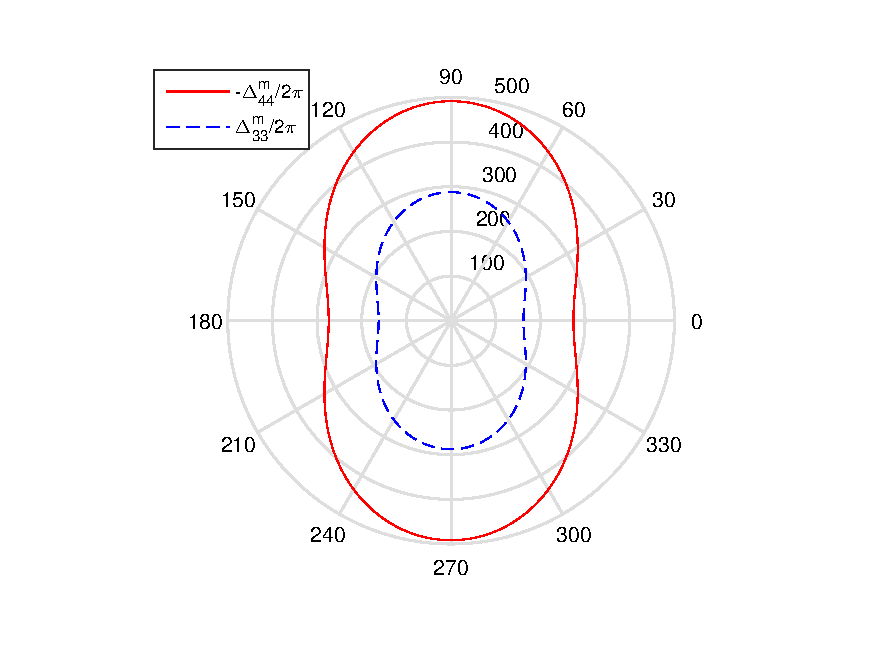
\includegraphics[scale=0.45]{./Figs/domega_magic12_q_NA2500_r1d8a}}
\end{minipage}
\begin{minipage}{.49\linewidth}
\centering
\subfloat[]{\label{fig:phiq_optimal_NA1000to5000_rp}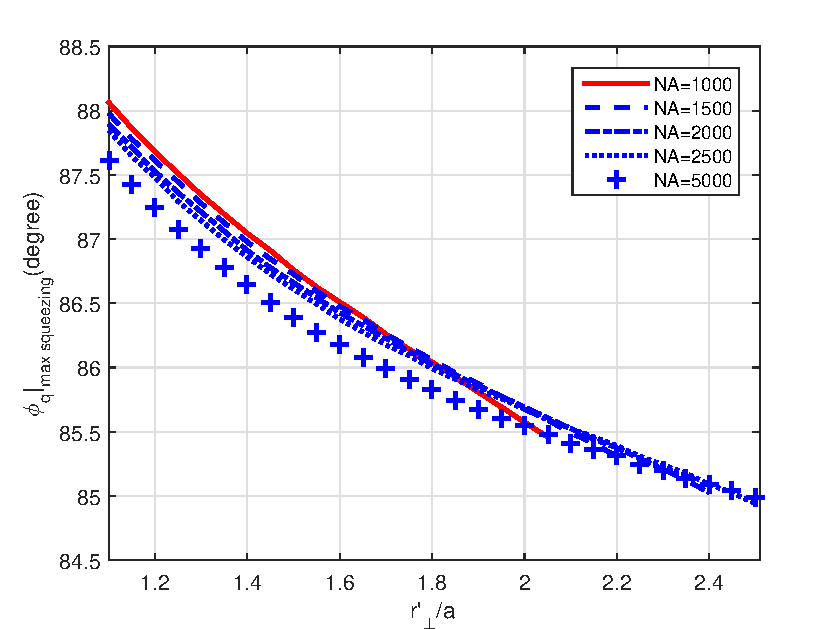
\includegraphics[scale=0.45]{./Figs/phiq_optimal_NA1000to5000_rp}}
\end{minipage}
\par\medskip
\begin{minipage}{.49\linewidth}
\centering
\subfloat[]{\label{fig:domega_magic44_qXYoptimal_rp}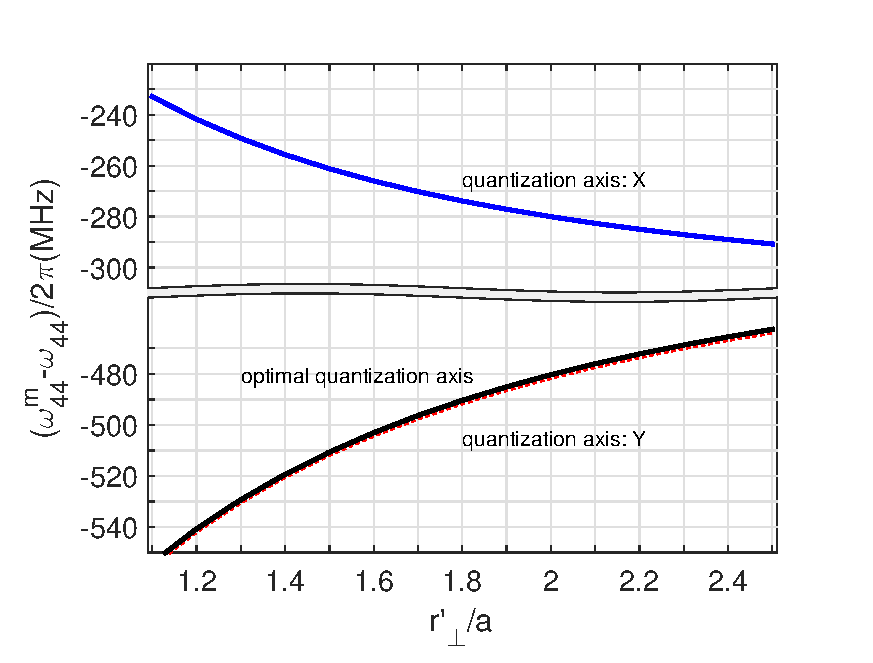
\includegraphics[scale=0.45]{./Figs/domega_magic44_qXYoptimal_rp}}
\end{minipage}
\begin{minipage}{.49\linewidth}
\centering
\subfloat[]{\label{fig:domega_magic33_qXYoptimal_rp}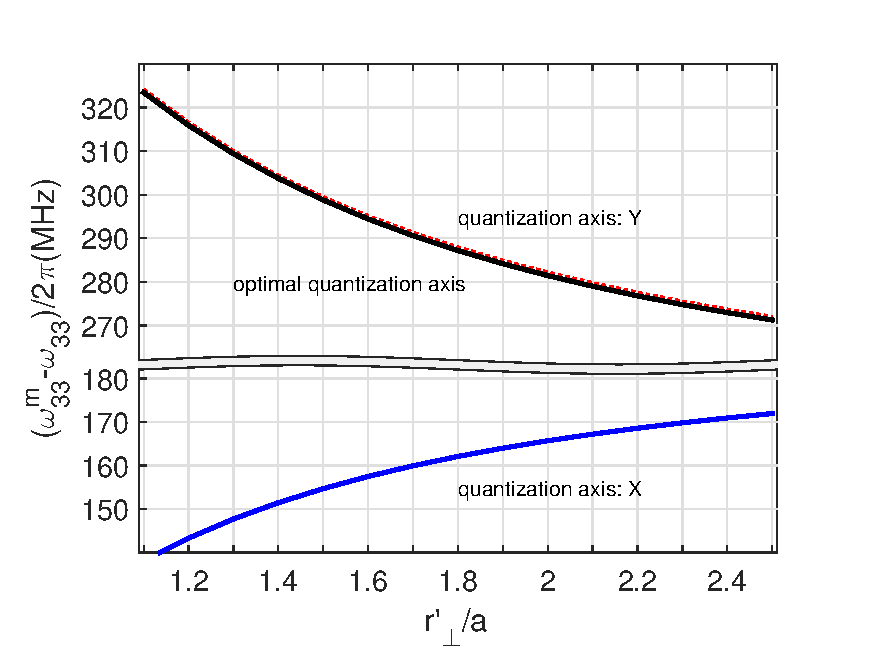
\includegraphics[scale=0.45]{./Figs/domega_magic33_qXYoptimal_rp}}
\end{minipage}
\caption{Subfig.~\protect\subref{fig:domega_magic12_q_NA2500_r1d8a} shows the magic detuning $ \Delta_{44}^m/2\pi=(\omega_{44}^m-\omega_{44})/2\pi $ and $ \Delta_{33}^m/2\pi=(\omega_{33}^m-\omega_{33})/2\pi $ as the quantization axis rotating in the $ xy $-plane while the atom is sitting at $ r'\!_\perp=1.8a $ position. Subfig.~\protect\subref{fig:phiq_optimal_NA1000to5000_rp} indicates the angle on the $ xy $-plane of the optimal quantization axis to achieve the maximal peak spin squeezing parameter. Lines are cut off when the spin squeezing parameter is effectively zero. Subfig.~\protect\subref{fig:domega_magic44_qXYoptimal_rp} shows the magic frequency detuning $ \Delta_{44}^m/2\pi $ as a function of atom position for using different quantization axis. Similar to subfig.~\protect\subref{fig:domega_magic44_qXYoptimal_rp}, subfig.~\protect\subref{fig:domega_magic33_qXYoptimal_rp} is the case of $ \Delta_{33}^m/2\pi $. }\label{fig:optimalq_domega_magics}
\end{figure}

\begin{figure}
\begin{minipage}{.49\linewidth}
\centering
\subfloat[]{\label{fig:xi_q_D1_NA2500_r1d8a}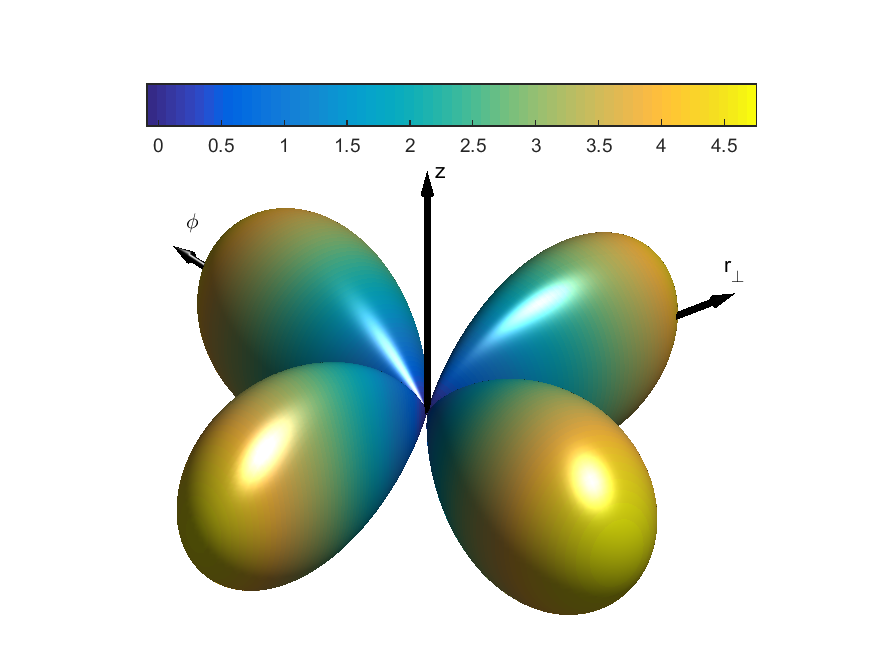
\includegraphics[scale=0.45]{./Figs/xi_q_D1_NA2500_r1d8a}}
\end{minipage}
\begin{minipage}{.49\linewidth}
\centering
\subfloat[]{\label{fig:ximax_q_D1_xyplane_NA2500_r1d8a}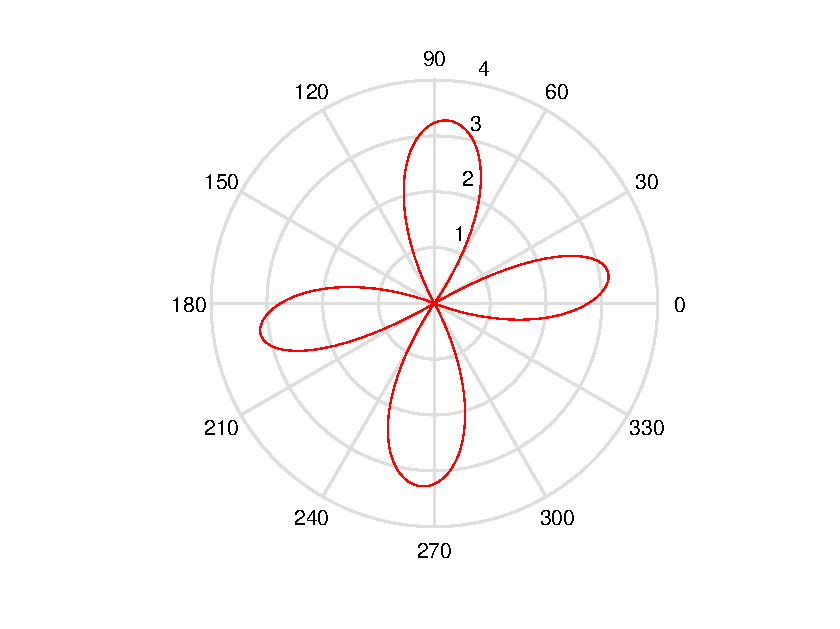
\includegraphics[scale=0.45]{./Figs/ximax_q_D1_xyplane_NA2500_r1d8a}}
\end{minipage}
\par\medskip
\begin{minipage}{.49\linewidth}
\centering
\subfloat[]{\label{fig:gamma34_q_D1_xyplane_NA2500_r1d8a_m44}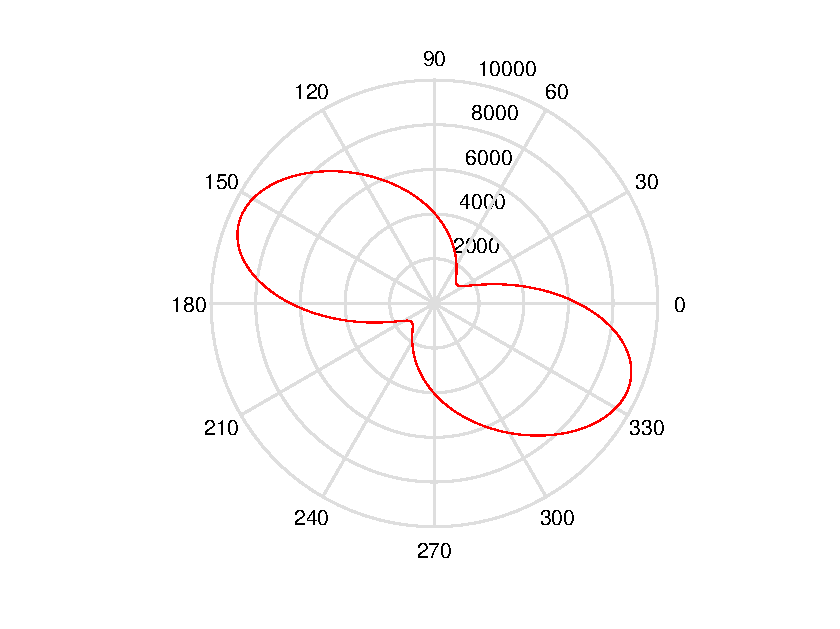
\includegraphics[scale=0.45]{./Figs/gamma34_q_D1_xyplane_NA2500_r1d8a_m44}}
\end{minipage}
\begin{minipage}{.49\linewidth}
\centering
\subfloat[]{\label{fig:OD_q_xyplane_r1d8a_m44}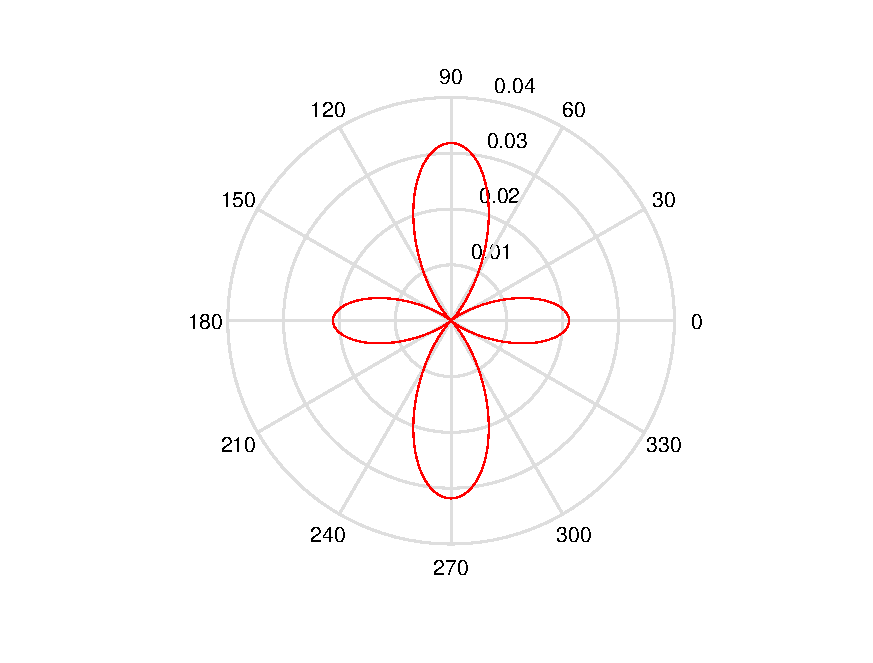
\includegraphics[scale=0.45]{./Figs/OD_q_xyplane_r1d8a_m44}}
\end{minipage}
\caption{Study of squeezing parameters with rotating quantization axis with $2500$ atoms positioned at $ r'\!_\perp=1.8a $. The magic frequency close to the $ F=4 \leftrightarrow F'=4$ transition of $ \mathrm{D}_1 $ line is used. Subfig.~\protect\subref{fig:xi_q_D1_NA2500_r1d8a} shows the squeezing parameter $ \xi^2 $ as the quantization axis rotates in the 3D space. Subfig~\protect\subref{fig:ximax_q_D1_xyplane_NA2500_r1d8a} gives the squeezing parameter when the quantization axis rotates on the $ xy $-plane. Subfig.~\protect\subref{fig:gamma34_q_D1_xyplane_NA2500_r1d8a_m44} is the spin flipping rate $ \gamma_{4\rightarrow 3} $ (in arbitrary units) as a function of the orientation of the quantization axis rotating in the $ xy $-plane. $ \gamma_{3\rightarrow 4} $ is very small compared to $ \gamma_{4\rightarrow 3} $ due to its far detuning. Subfig.~\protect\subref{fig:OD_q_xyplane_r1d8a_m44} shows the $ \mathrm{OD}/{\mathrm{atom}}=\kappa/\gamma_s $ when the quantization axis is rotating in the $ xy $-plane.  }\label{fig:squeezing_q_D1_NA2500_r1d8a}
\end{figure}

%================
\begin{figure}
\begin{minipage}{.49\linewidth}
\centering
\subfloat[]{\label{fig:xi_optimal_NA1000to5000_omega44}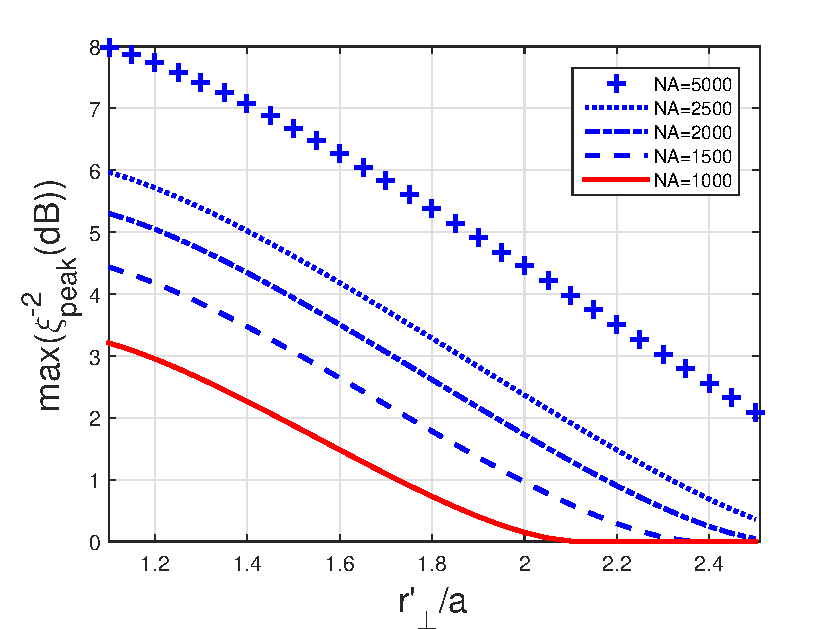
\includegraphics[scale=0.45]{./Figs/xi_optimal_NA1000to5000_omega44}}
\end{minipage}
\begin{minipage}{.49\linewidth}
\centering
\subfloat[]{\label{fig:OD_optimal_rp}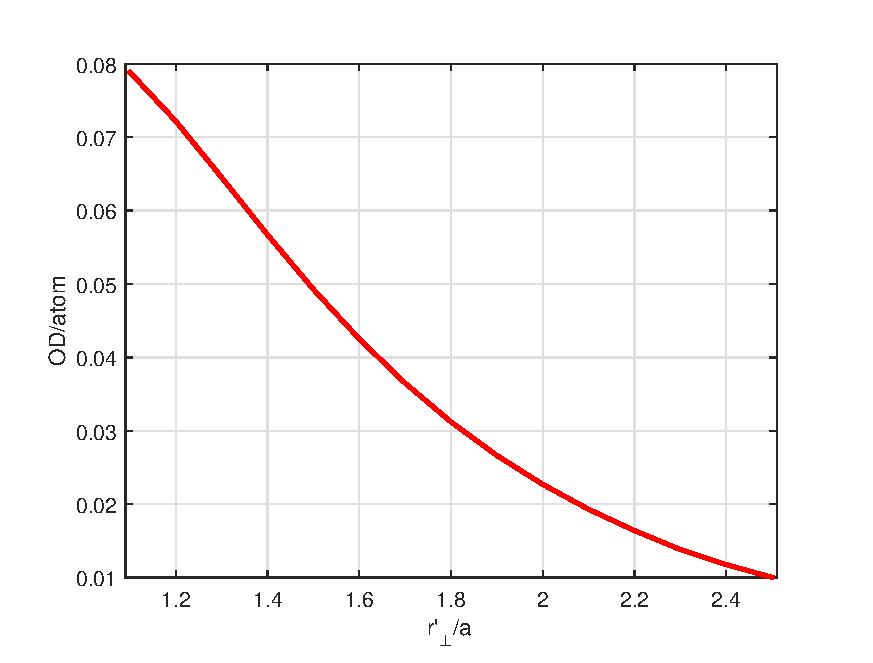
\includegraphics[scale=0.45]{./Figs/OD_optimal_rp}}
\end{minipage}
\caption{QND measurement properties using the magic frequency $ \omega_{44} $. Subfigure~\protect\subref{fig:xi_optimal_NA1000to5000_omega44} shows the optimal peak spin squeezing parameter as a function of the radial position of the atom. Different atom numbers have been indicated in different types of lines. Subfigure~\ref{fig:OD_optimal_rp} shows the OD per atom parameter, $ \mathrm{OD}/{\mathrm{atom}}\equiv \kappa/\gamma_s= \sigma_0A_{\rm in}/4A_{\rm eff}^2 $, as a function of atoms' radial position when the optimal quantization axis is chosen to plot Subfig.~\protect\subref{fig:xi_optimal_NA1000to5000_omega44}. }\label{fig:QNDproperty_magic44}
\end{figure}
%================


\begin{figure}
\begin{minipage}{.49\linewidth}
\centering
\subfloat[]{\label{fig:xit_qXoptimal_r1d8a_NA2500}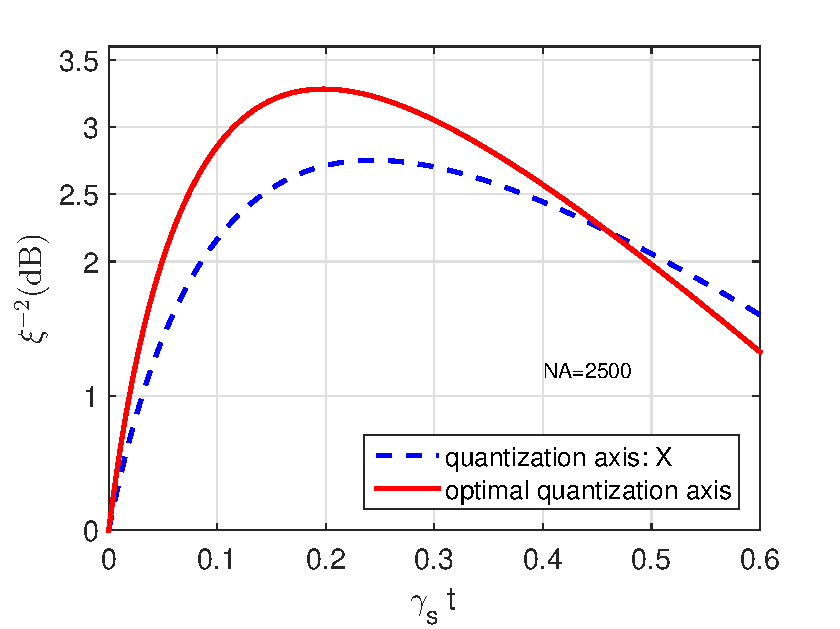
\includegraphics[scale=0.45]{./Figs/xit_qXoptimal_r1d8a_NA2500}}
\end{minipage}
\begin{minipage}{.49\linewidth}
\centering
\subfloat[]{\label{fig:DeltaJz2t_qXoptimal_r1d8a_NA2500}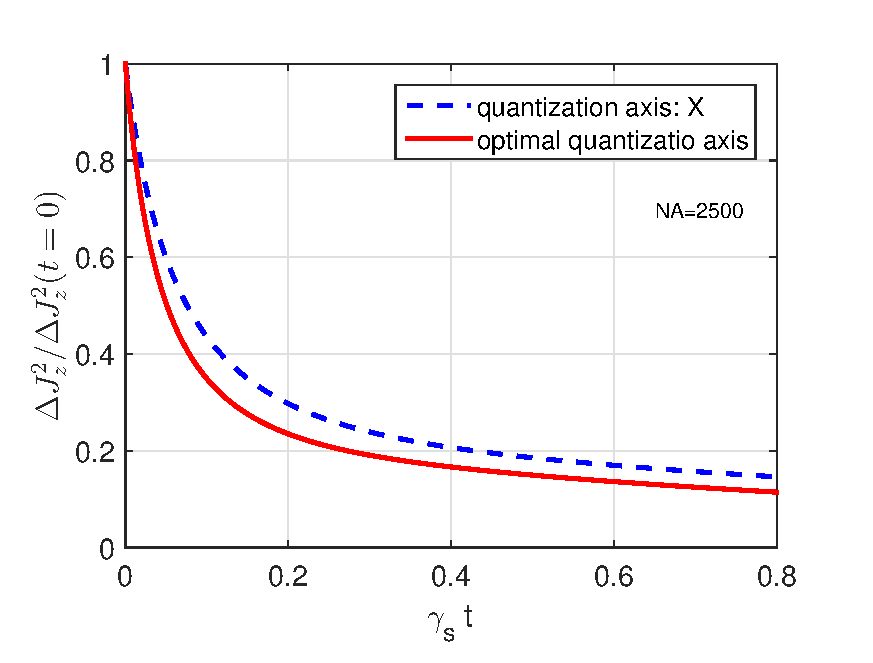
\includegraphics[scale=0.45]{./Figs/DeltaJz2t_qXoptimal_r1d8a_NA2500}}
\end{minipage}
\par\medskip
\begin{minipage}{.49\linewidth}
\centering
\subfloat[]{\label{fig:Jxt_qXoptimal_r1d8a_NA2500}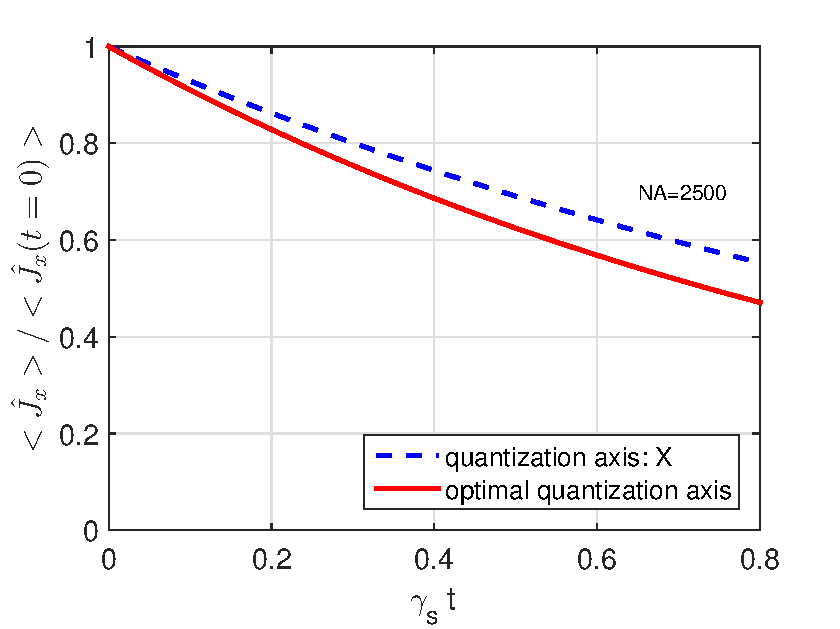
\includegraphics[scale=0.45]{./Figs/Jxt_qXoptimal_r1d8a_NA2500}}
\end{minipage}
\begin{minipage}{.49\linewidth}
\centering
\subfloat[]{\label{fig:NAt_qXoptimal_r1d8a_NA2500}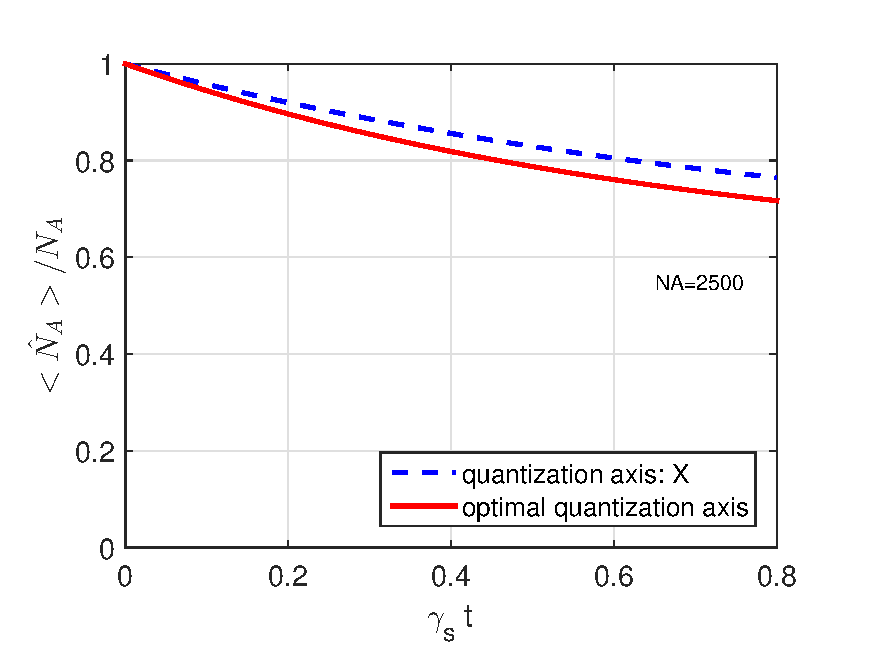
\includegraphics[scale=0.45]{./Figs/NAt_qXoptimal_r1d8a_NA2500}}
\end{minipage}
\caption{Dynamics of spin squeezing parameter and expectation values of spin operators for the birefringence metrology using $ x $-axis and the optimal quantization axis as the quantization axis with $ 2500 $ atoms positioned at $ r'\!_\perp=1.8a $ radial distance. Subfig.~\protect\subref{fig:xit_qXoptimal_r1d8a_NA2500} shows the dynamics of the spin squeezing parameter. Subfigs.~\protect\subref{fig:DeltaJz2t_qXoptimal_r1d8a_NA2500},~\protect\subref{fig:Jxt_qXoptimal_r1d8a_NA2500} and~Subfigs.~\protect\subref{fig:NAt_qXoptimal_r1d8a_NA2500} are for $ \Delta J_z^2 $, $ \expect{\hat{J}_x} $ and $ \expect{\hat{N}_A} $ normalized to their initial values, respectively. }\label{fig:clockdynamics_q_r1d8a}
\end{figure}



\begin{figure}
\begin{minipage}{.49\linewidth}
\centering
\subfloat[]{\label{fig:xit_q_r1d8a_NA2500}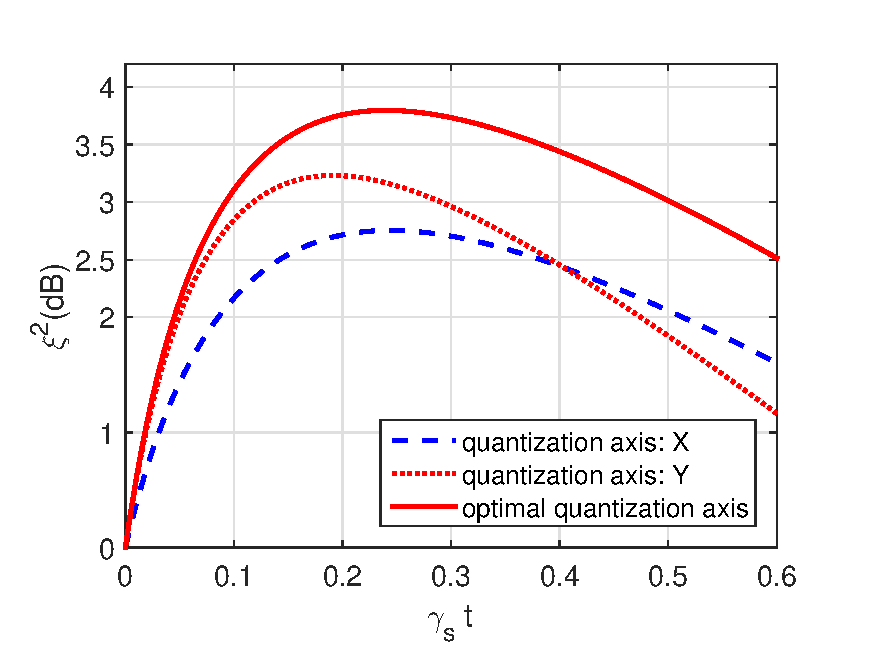
\includegraphics[scale=0.45]{./Figs/xit_q_r1d8a_NA2500}}
\end{minipage}
\begin{minipage}{.49\linewidth}
\centering
\subfloat[]{\label{fig:xit_qoptimal_r1d8a_NA1000to5000}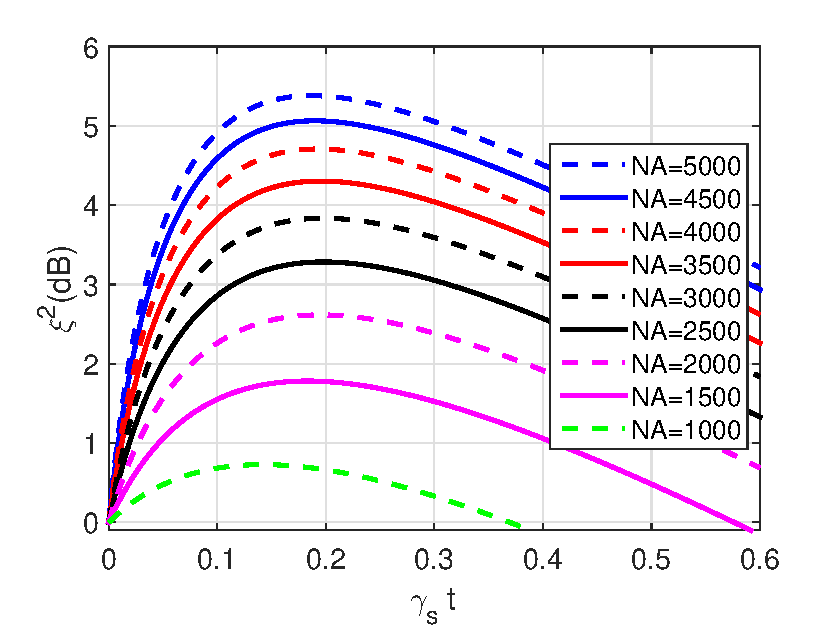
\includegraphics[scale=0.45]{./Figs/xit_qoptimal_r1d8a_NA1000to5000}}
\end{minipage}
\caption{Dynamics of spin squeezing parameter $ \xi^2 $ with atoms placed at $ r'\!_\perp=1.8a $ position for the birefringence metrology. Subfig.~\protect\subref{fig:xit_q_r1d8a_NA2500} uses $ 2500 $ atoms while changing the quantization axis in the $ xy $-plane. Subfig.~\protect\subref{fig:xit_qoptimal_r1d8a_NA1000to5000} uses the optimal spin squeezing quantization axis yet with various atom numbers. }\label{fig:xit_r1d8a}
\end{figure}


\missingfigure{Poincare sphere diagram with spin squeezing effect.}

\missingfigure{Plots for $N^{min}_A$.}

\subsection{Other applications?} 


\section{SUMMARY and OUTLOOK}

Outside of a waveguide, cavity enhancement can produce drastic increases in atom-number detection, \cite{zhang_collective_2012}, spin squeezing \cite{bohnet_reduced_2014}, and....   Strong coupling to the guided nanofiber modes can be further improved with nanofabricated cavities that, under EIT conditions, substantially slow the group velocity \cite{le_kien_intracavity_2009,wuttke_nanofiber_2012,nayak_optical_2014}.  Additional hybrid approaches \cite{hafezi_atomic_2012, yalla_cavity_2014}.  Coherent quantum control of atoms \cite{smith_quantum_2013-1}.  Quantum sensing \cite{kumar_autler-townes_2015}.  Preparation of nonclassical light using collective dissipation \cite{gonzalez-tudela_deterministic_2015}.  Optical memory (not quite quantum) \cite{sayrin_storage_2015, gouraud_demonstration_2015} Interaction with higher-order modes.  Optical switching using a single atom \cite{oshea_fiber-optical_2013} 

Optical pumping near the surface of a dielectric that modifies the local density of states, 

Initial state preparation can improve the precision of dispersive atom number measurements, 

\cite{scheel_directional_2015}
\comment{Any discussion of metallic nanowires?}

\comment{
OTHER FIGURES FOR ELSEWHERE IN PAPER \\
\emph{Figure}: Nanofiber schematic \\
\emph{Figure}: Phase shift \\
\emph{Figure}: Atom number resolution \\
\emph{Figure}: Atomic structure \\
a) clock-state level structure and $H,V$-transitions \\
b) magic wavelength (in detuning) as a function of quantization axis $\phi_Q$ in $x,y$-plane \\
c) magic wavelength (in detuning) as a function of distance from the fiber $r_\perp/a$ for fixed $\phi_Q$ 

}

%\begin{center}
%{\bf References}
%\end{center}

%\bibliography
%\bibliographystyle{amsplain}
\bibliographystyle{unsrt}
\bibliography{Nanofibers}
% \nocite{*}
%\ifwindows
%	\bibliography{F:/References/Archive/Archive}
%\else
%	\bibliography{/media/F/References/Archive/Archive}
%\fi

%====== APPENDIX =========
\begin{appendix}	

%===================APPENDIX: Nanofiber mode functions=====================%
\section{Guided-mode functions for the optical nanofiber} \label{Appendix::ModeFunctions}

Here we briefly review the guided-mode eigenfunctions for an optical nanofiber.  The nanofiber's distinguishing feature that the diameter is smaller than the operating wavelength of light has several consequences.  First, a significant fraction of the transmitted power resides in evanescent fields that can extend well beyond the nanofiber's surface.  This evanescent field is the tool with which atoms are trapped and manipulated by fiber-guided light.  Second, the guided modes outside the taper region adiabatically transform through the fiber taper into the modes of the nanofiber without significant losses.  Through this transformation, the guided fields acquire a large component along the fiber axis that is out of phase with the transverse components, which makes the nanofiber modes significantly different from the transverse plane waves or paraxial modes in free space.    

Here, we provide the fundamental HE$_{11}$ solutions to the homogeneous wave equation, \erf{Eq::WaveEquationSource} with $\tensor{\boldsymbol{\alpha}} = 0$, for a cylindrical nanofiber of radius $a$ and index of refraction given by \erf{Eq::IndexofRefraction}.  At a given frequency, $\omega_0 = c k_0$, the magnitudes of the longitudinal and transverse wave vectors for a guided mode are related by $n^2 k_0^2 = \beta_0^2 + k_\perp^2$.  The positive propagation constant, $\beta_0 \equiv \beta(\omega_0)$, is determined from the eigenvalue equation that results from enforcing physical boundary conditions at the fiber surface \cite{Yariv, Marcuse, Snyder and Love},
	\begin{align}
		\frac{J_0(ha)}{ha J_1(ha)} = - \frac{n_1^2+n_2^2}{2n_1^2} \frac{K'(qa)}{qa K_1(qa)} + \frac{1}{h^2 a^2} - \bigg[ \bigg(\frac{n_1^2 - n_2^2}{2 n_1^2} \frac{K'(qa)}{qa K_1(qa)} \bigg)^2  + \frac{\beta_0^2}{n^2_1 k^2} \bigg(\frac{1}{q^2a^2} + \frac{1}{h^2a^2} \bigg)^2 \bigg]^{1/2}.
	\end{align}
Inside the nanofiber the transverse wavevector is real, $k_\perp = q$, where $q=\sqrt{\beta_0^2- n_2^2k_0^2}$, and outside the nanofiber it is purely imaginary, $k_\perp = i h$, where $h=\sqrt{n_1^2 k_0^2 - \beta_0^2}$.  The vector eigenfunctions are expressed as $\mbf{f}_{\mu}(\br) = (2\pi)^{-1/2}\mbf{u}_{f,p}(\mbf{r}_\perp) e^{i f \beta_0 z}$, where the modes are indexed by frequency $\omega_0$, propagation direction $f = \pm$, and polarization $p$.

A relatively simple form for the guided-mode functions can be expressed in a cylindrical basis $(r_\perp, \phi, z)$ with longitudinal unit vector $\mathbf{e}_z$, oriented along the fiber axis.  The transverse unit vector are related to their fixed Cartesian counterparts via the relations
	\begin{align}
		\mathbf{e}_r     &= \mathbf{e}_x \cos \phi + \mathbf{e}_y \sin \phi, \\
		\mathbf{e}_\phi &= - \mathbf{e}_x \sin \phi + \mathbf{e}_y \cos \phi.
	\end{align}
\comment{Please check all the signs, as I modified the phase conventions from Le Kien's in order to make all the profile functions real.}  The transverse profile for the quasicircular guided modes, $p = \pm$, is
	\begin{align} \label{Eq::QuasicircularModes}
		\mbf{u}_{f,\pm}(\mathbf{r}) = \big[\mathbf{e}_r u_r(r_\perp) \pm i \mathbf{e}_\phi u_\phi(r_\perp) +  i f \mathbf{e}_z  u_z(r_\perp) \big]e^{ \pm i \phi}, 
	\end{align}
and for the quasilinear guided modes, $p = \{H,V\}$, is
	\begin{subequations} \label{Eq::QuasilinearModes}
	\begin{align}
		\mbf{u}_{f,H}(\mathbf{r}) = & \sqrt{2} \big[ \mathbf{e}_r u_r(r_\perp) \cos \phi - \mathbf{e}_\phi u_\phi(r_\perp) \sin \phi +  if \mathbf{e}_z  u_z(r_\perp) \cos \phi \big] \\
		\mbf{u}_{f,V}(\mathbf{r}) = & \sqrt{2} \big[ \mathbf{e}_r u_r(r_\perp) \sin \phi + \mathbf{e}_\phi u_\phi(r_\perp) \cos \phi +  if \mathbf{e}_z  u_z(r_\perp) \sin \phi \big]. 
	\end{align}
	\end{subequations}
The modes have been expressed in terms of real-valued functions that depend only on the radial coordinate $r_\perp$,
	\begin{subequations} \label{Eq::ProfileFunctions}
	\begin{align} 
		u_r(r_\perp) =& u_0 \big[ (1-s) K_0(qr) + (1+s)K_2(qr)\big] \\
		u_\phi(r_\perp) =& u_0\big[ (1-s) K_0(qr) - (1+s)K_2(qr)\big] \\
		u_z(r_\perp) =& u_0 \frac{2 q}{\beta_0} \frac{K_1(qa)}{J_1(ha)} J_1(hr), \label{Eq::zprofile}
	\end{align}
	\end{subequations}
where $u_0$ is set by the normalization condition, $\int d^2 \mathbf{r}_\perp n(r_\perp) | \mathbf{u}_\mu(\br_\perp)|^2=1$, $J_n$ and $K_n$ are the $n^{th}$ Bessel functions of the first and second kind, $f'(x)$ indicates a derivative with respect to the argument $x$, and 
	\begin{align}
		s = \frac{1/(q^2 a^2)^{2} + 1/(h^2 a^2)^{2}}{[J'_1(ha)/haJ_1(ha) + K'_1(qa)/qaK_1(qa)]}.
	\end{align}  
Of particular interest is the $z$-component, \erf{Eq::zprofile}, which can become appreciable.  Note that the phase convention in Eqs. (\ref{Eq::QuasicircularModes}-\ref{Eq::ProfileFunctions}) has been chosen to emphasize properties of the quasilinear modes and differs from that of \emph{Le Kien et al.} -- for instance, in Ref. \cite{le_kien_propagation_2014}.  Further details about the guided-mode fields inside the nanofiber ($r_\perp\leq a$), the radiation (unguided) modes, and the quantized form of both can be found in Refs. \cite{sondergaard_general_2001, tong_single-mode_2004, kien_field_2004, le_kien_spontaneous_2005, Vetsch thesis}.

\change{
%===================APPENDIX: Mode area =====================%
\section{Master equation for optical pumping} \label{Appendix::Optical pumping}

The master equation that describes optical pumping of an alkali atom driven by an off-resonant monochromatic laser \cite{deutsch_quantum_2010}
	\begin{align}
		\frac{d \hat{\rho}^{(n)}  }{dt}\Big|_{\rm op} = 
		&-\frac{i}{\hbar} \big\{ \hat{H}_{\rm loss},\hat{\rho}^{(n)} \big\}_+ + \sum_q \sum_{F_a,F_b} \hat{W}_{F_aF_b} \hat{\rho}^{(n)} \hat{W}\dg_{F_aF_b} \\
		= & \sum_{F} -\frac{\gamma_F}{2} \big\{ \op{F,0}{F,0},\hat{\rho}^{(n)} \big\}_+ + \sum_{F_a,F_b} \gamma_{F_a \rightarrow F_b} \op{F_b,0}{F_a,0} \hat{\rho}^{(n)} \op{F_a,0}{F_b,0} \\
	\end{align}	
		
Jump operators
	\begin{align}
%		\hat{W}^q = \sum_{e} \sqrt{ \frac{\Gamma_e \Omega^2(\mathbf{r}')/4}{\Delta^2_{ge} + \Gamma^2_e/4}} \mbf{e}_q^* \cdot \mbf{d}\dg \mbf{d} \cdot \vec{\varepsilon}_\inp
		\hat{W}_{g_1,g_2} = \sqrt{\gamma_{g_1 \rightarrow g_2}} \op{g_2}{g_1}
	\end{align}
Transition rate
	\begin{align}
		\gamma_{g_1 \rightarrow g_2} = \sum_q \sum_e \Gamma_e \frac{ \Omega^2(\mathbf{r}')/4}{\Delta^2_{eg_1} + \Gamma^2_e/4} \big|  \mbf{e}_q^* \cdot \bra{g_2} \hat{\mbf{D}} \op{e}{e}\hat{\mbf{D}}  \ket{g_1} \cdot \vec{\varepsilon}_\inp \big|^2
	\end{align}
where the spherical unit vectors, $\mbf{e}_q$, determine the $\{\pi, \sigma_+, \sigma_-\}$-transition rates for the chosen quantization axis.


%===================APPENDIX: Mode area =====================%
\section{Effective cross-sectional mode area} \label{Appendix::ModeArea}
In the photonic crystal literature, the effective mode area is defined as \cite{goban_atomlight_2014}
	\begin{align}
		A_\eff \equiv \frac{n_g \sigma_0}{2} \frac{\Gamma_0}{\Gamma_\oneD(\mathbf{r})}
	\end{align}
or as \cite{manga_rao_single_2007}
	\begin{align}
		A_\eff \equiv \frac{1}{ \mbox{max} \big[ n^2(\mathbf{r}) |\mathbf{f}_\eta(\mathbf{r})|^2 \big]}
	\end{align}
or as \cite{hung_trapped_2013}
	\begin{align}
		A_\eff \equiv \int d^2 \mathbf{r}_\perp \frac{n^2(\mathbf{r}) |\mathbf{E}(\mathbf{r})|^2 }{n^2(\mathbf{r}_{\rm min}) |\mathbf{E}(\mathbf{r}_{\rm min})|^2 } =  \frac{P_\inp}{ n_g  I_\inp(\mathbf{r}_{\rm min}) }.
	\end{align}
	
Within the secular approximation, the result of the ground hyperfine multiplets being separated in energy is that populations within each manifold only feed populations, and coherences between the manifolds only feed coherences \cite{deutsch_quantum_2010}.  
}

\end{appendix}

\end{document}